\documentclass[UTF8,11pt]{ctexart}
\usepackage[a4paper,margin=19mm]{geometry}
\usepackage{amsmath,amssymb,tikz,graphicx,hyperref}
\usetikzlibrary{arrows.meta,decorations.pathmorphing}
\setlength{\parindent}{0pt}\setlength{\parskip}{6pt}
\sloppy\emergencystretch=3em

% Site layout only: preserve text, mathematics and native chemical diagrams.
\setlength{\parskip}{2pt}
\raggedbottom
\let\originalenumerate\enumerate
\renewcommand{\enumerate}{\originalenumerate
 \setlength{\itemsep}{2pt}\setlength{\parsep}{0pt}\setlength{\topsep}{3pt}}
\makeatletter
\renewcommand\subsection{\@startsection{subsection}{2}{\z@}
 {-1.1ex\@plus -.3ex\@minus -.2ex}{.5ex\@plus .2ex}
 {\normalfont\normalsize\bfseries}}
\makeatother

\begin{document}\newsavebox{\mockquestionbox}
\begin{center}{\LARGE 南京工业大学637有机化学}\par\medskip{\Large D21 强化型模拟卷 详细解析}\par\medskip 满分150分\quad 考试时间180分钟\end{center}本解析供交卷后核对。采分点为训练建议，不是学校官方评分。等效、化学成立且满足题限的解法应酌情给分。\par\section*{一、填空、命名与完成反应（15题，共30分）}\subsection*{1．（2分）}完成下列反应，注意立体构型。\begin{center}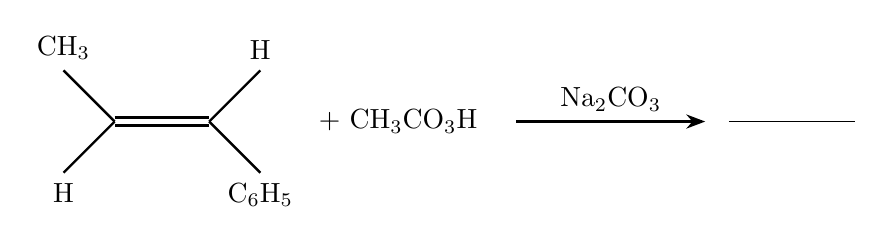
\begin{tikzpicture}[line width=.85pt,>=Stealth]\draw[double,double distance=2pt](-.6,0)--(.6,0);\draw(-.6,0)--(-1.25,.65)node[above]{$\mathrm{CH_3}$};\draw(-.6,0)--(-1.25,-.65)node[below]{$\mathrm{H}$};\draw(.6,0)--(1.25,.65)node[above]{$\mathrm{H}$};\draw(.6,0)--(1.25,-.65)node[below]{$\mathrm{C_6H_5}$};\node at(3,0){$+\ \mathrm{CH_3CO_3H}$};\draw[->](4.5,0)--(6.9,0)node[midway,above]{$\mathrm{Na_2CO_3}$};\node at(8,0){\rule{1.6cm}{.3pt}};\end{tikzpicture}\end{center}\subsection*{答案与结构}生成trans-2-甲基-3-苯基环氧乙烷的一对对映体（外消旋）。图示一个，另一个全部立体中心反转。\begin{center}\begin{tikzpicture}[line width=.85pt,>=Stealth]\draw(-.65,.35)--(.65,.35)--(0,-.65)--cycle;\node[fill=white,inner sep=1pt]at(0,-.65){$\mathrm{O}$};\foreach\t in{.2,.4,.6,.8,1}{\draw(-.65-.65*\t-.07*\t,.35+.65*\t+.07*\t)--(-.65-.65*\t+.07*\t,.35+.65*\t-.07*\t);}\node[above left]at(-1.3,1){$\mathrm{CH_3}$};\fill(.65,.35)--(1.23,1.07)--(1.37,.93)--cycle;\node[above right]at(1.3,1){$\mathrm{Ph}$};\node at(3,0){及其镜像（外消旋）};\end{tikzpicture}\end{center}\subsection*{从概念到解法}\begin{enumerate}\item 过氧乙酸把一个O转移到双键两碳，协同生成两个C-O键和三元环。此反应保持烯烃取代基之间的相对空间关系。\item 原底物Me和Ph跨双键相反，为E型；因此环氧化后两者仍处于三元环两侧，不能画成cis。\item 平面烯烃在无手性环境中可从两面受氧转移，得到互为镜像的两个trans构型。Na2CO3用于缓冲酸性；没有强酸开环步骤，终点为环氧化物。\end{enumerate}\subsection*{验算与易错}加一个O，C9骨架无断裂。；Me/Ph为trans且写出镜像，不把一张楔线图误当唯一构型。\subsection*{参考采分（非官方）}环氧连接1分；trans及外消旋1分。\par 来源：S01，8-59(viii)，印刷页148，PDF页154。\par\medskip\clearpage\subsection*{2．（2分）}完成下列反应，写出主要产物，并指出此反应是亲核加成还是亲电加成，是1,2-加成还是1,4-加成。\begin{center}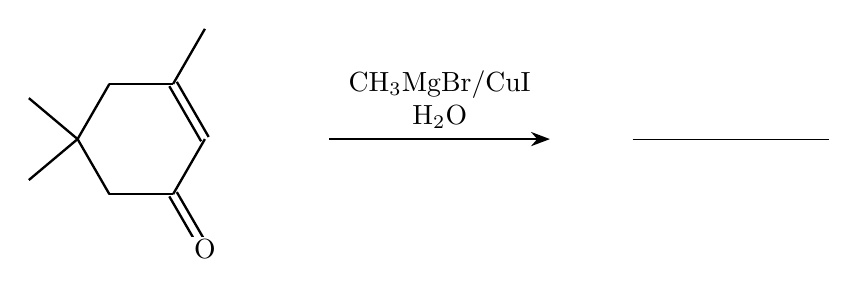
\begin{tikzpicture}[line width=.85pt,>=Stealth]\draw (1.166,-1.372)--(0.761,-0.673);
\draw (1.070,-1.427)--(0.666,-0.728);
\draw (0.714,-0.700)--(1.118,-0.000);
\draw (1.166,0.027)--(0.761,0.727);
\draw (1.070,-0.028)--(0.666,0.672);
\draw (0.714,0.700)--(1.118,1.400);
\draw (0.714,0.700)--(-0.095,0.700);
\draw (-0.095,0.700)--(-0.499,-0.000);
\draw (-0.499,-0.000)--(-1.118,-0.520);
\draw (-0.499,-0.000)--(-1.118,0.520);
\draw (-0.499,-0.000)--(-0.095,-0.700);
\draw (-0.095,-0.700)--(0.714,-0.700);
\node[fill=white,inner sep=1.1pt]at(1.118,-1.400){$\mathrm{O}$};\draw[->](2.7,0)--(5.5,0)node[midway,above,align=center]{$\mathrm{CH_3MgBr/CuI}$\\$\mathrm{H_2O}$};\node at(7.8,0){\rule{2.5cm}{.3pt}};\end{tikzpicture}\end{center}\subsection*{答案与结构}产物为3,3,5,5-四甲基环己酮；属于亲核1,4-加成。\begin{center}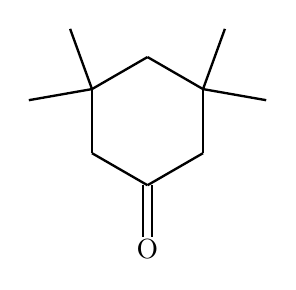
\begin{tikzpicture}[line width=.85pt,>=Stealth]\draw (0.055,-1.400)--(0.055,-0.586);
\draw (-0.055,-1.400)--(-0.055,-0.586);
\draw (0.000,-0.586)--(0.705,-0.179);
\draw (0.705,-0.179)--(0.705,0.635);
\draw (0.705,0.635)--(0.983,1.400);
\draw (0.705,0.635)--(1.507,0.494);
\draw (0.705,0.635)--(-0.000,1.042);
\draw (-0.000,1.042)--(-0.705,0.635);
\draw (-0.705,0.635)--(-1.507,0.494);
\draw (-0.705,0.635)--(-0.983,1.400);
\draw (-0.705,0.635)--(-0.705,-0.179);
\draw (-0.705,-0.179)--(0.000,-0.586);
\node[fill=white,inner sep=1.1pt]at(0.000,-1.400){$\mathrm{O}$};\end{tikzpicture}\end{center}\subsection*{从概念到解法}\begin{enumerate}\item 先把共轭羰基标成O-C(=O)-C\(\alpha\)=C\(\beta\)。CuI使有机镁试剂表现为有机铜型较软亲核体，常优先进攻\(\beta\)碳。\item 新增Me接到原\(\beta\)碳，即原来已经带Me的烯碳；C=C移电子形成烯醇盐，经水处理恢复酮。\item 所以原\(\beta\)碳变成偕二甲基，另一个原偕二甲基保留；不是羰基碳加Me形成叔醇。\end{enumerate}\subsection*{验算与易错}9C底物加1C到10C，氧仍为酮氧。；C=C被消耗，C=O保留，与1,4而非1,2一致。\subsection*{参考采分（非官方）}产物1分；亲核及1,4各0.5分。\par 来源：S01，10-17(vii)，印刷页188，PDF页194。\par\medskip\clearpage\subsection*{3．（2分）}完成下列反应，写出主要产物。\begin{center}\begin{tikzpicture}[line width=.85pt,>=Stealth]\draw (2.000,0.098)--(1.353,0.244);
\draw (1.353,0.244)--(1.091,0.854);
\draw (1.091,0.854)--(0.430,0.794);
\draw (0.430,0.794)--(0.283,0.146);
\draw (0.283,0.146)--(-0.327,-0.116);
\draw (-0.381,-0.109)--(-0.459,-0.768);
\draw (-0.272,-0.122)--(-0.350,-0.781);
\draw (-0.327,-0.116)--(-0.858,0.281);
\draw (-0.858,0.281)--(-1.468,0.019);
\draw (-1.468,0.019)--(-2.000,0.417);
\draw (0.283,0.146)--(0.854,-0.193);
\draw (0.799,-0.198)--(0.860,-0.859);
\draw (0.908,-0.188)--(0.969,-0.849);
\draw (0.854,-0.193)--(1.353,0.244);
\node[fill=white,inner sep=1.1pt]at(-0.405,-0.775){$\mathrm{O}$};
\node[fill=white,inner sep=1.1pt]at(-0.858,0.281){$\mathrm{O}$};
\node[fill=white,inner sep=1.1pt]at(0.914,-0.854){$\mathrm{O}$};\draw[->](2.7,0)--(5.5,0)node[midway,above,align=center]{$2\mathrm{KNH_2}$/液氨\\(1)$\mathrm{CH_3I}$ (2)$\mathrm{NH_4Cl}$};\node at(7.8,0){\rule{2.5cm}{.3pt}};\end{tikzpicture}\end{center}\subsection*{答案与结构}烷基化发生在原来带Me的酮\(\alpha\)碳，产物为该碳偕二甲基、另一\(\alpha\)碳保留COOEt的环戊酮。\begin{center}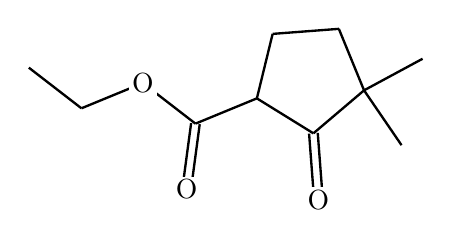
\begin{tikzpicture}[line width=.85pt,>=Stealth]\draw (2.500,0.704)--(1.757,0.303);
\draw (1.757,0.303)--(2.233,-0.393);
\draw (1.757,0.303)--(1.437,1.084);
\draw (1.437,1.084)--(0.596,1.020);
\draw (0.596,1.020)--(0.396,0.201);
\draw (0.396,0.201)--(-0.384,-0.120);
\draw (-0.439,-0.113)--(-0.551,-0.949);
\draw (-0.330,-0.127)--(-0.442,-0.963);
\draw (-0.384,-0.120)--(-1.052,0.396);
\draw (-1.052,0.396)--(-1.832,0.075);
\draw (-1.832,0.075)--(-2.500,0.591);
\draw (0.396,0.201)--(1.114,-0.243);
\draw (1.059,-0.247)--(1.123,-1.088);
\draw (1.169,-0.238)--(1.233,-1.080);
\draw (1.114,-0.243)--(1.757,0.303);
\node[fill=white,inner sep=1.1pt]at(-0.497,-0.956){$\mathrm{O}$};
\node[fill=white,inner sep=1.1pt]at(-1.052,0.396){$\mathrm{O}$};
\node[fill=white,inner sep=1.1pt]at(1.178,-1.084){$\mathrm{O}$};\end{tikzpicture}\end{center}\subsection*{从概念到解法}\begin{enumerate}\item \(\beta\)-酮酯中夹在两羰基之间的H首先被夺取，单负离子由两羰基离域稳定。\item 使用2当量KNH2可再夺去另一侧酮\(\alpha\)位的H，形成二负离子。后形成、较少稳定的碳负性位点在CH3I烷基化中反应，使原带Me的碳再接一个Me。\item NH4Cl使剩余烯醇盐质子化并恢复羰基。该条件区别于只用1当量碱时在两羰基之间进行烷基化；不能忽略2当量而选最酸H位作唯一进攻位。\end{enumerate}\subsection*{验算与易错}原酮\(\alpha\)碳已有Me，再接Me形成四键碳，不多加H。；产物保留酮与酯，两负电经烷基化、淬灭消失；总C增加1。\subsection*{参考采分（非官方）}正确区域1分；全部官能团和Me数量1分。\par 来源：S01，13-15(i)，印刷页260，PDF页266。\par\medskip\clearpage\subsection*{4．（2分）}完成反应。若有立体化学问题，应表明立体构型。\begin{center}\begin{tikzpicture}[line width=.85pt,>=Stealth]\draw(0,1)--(.87,.5)--(.87,-.5)--(0,-1)--(-.87,-.5)--(-.87,.5)--cycle;\fill(0,1)--(-.06,1.75)--(.06,1.75)--cycle;\node[above]at(0,1.75){$\mathrm{CH(CH_3)_2}$};\foreach\t in{.2,.4,.6,.8,1}{\draw(.87+.7*\t-.04*\t,.5+.4*\t+.07*\t)--(.87+.7*\t+.04*\t,.5+.4*\t-.07*\t);\draw(-.08*\t,-1-.7*\t)--(.08*\t,-1-.7*\t);}\node[right]at(1.57,.9){$\mathrm{Cl}$};\node[below]at(0,-1.7){$\mathrm{CH_3}$};\draw[->](2.4,0)--(4.5,0)node[midway,above]{$\mathrm{KOH}$}node[midway,below]{$\mathrm{EtOH}$};\node at(5.8,0){\rule{1.6cm}{.3pt}};\end{tikzpicture}\end{center}\subsection*{答案与结构}双键在原Cl所在碳与其下方无取代\(\beta\)碳之间；原iPr与Me的反面关系保留，见图。\begin{center}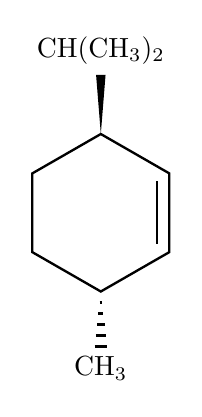
\begin{tikzpicture}[line width=.85pt,>=Stealth]\draw(0,1)--(.87,.5)--(.87,-.5)--(0,-1)--(-.87,-.5)--(-.87,.5)--cycle;\draw(.71,.4)--(.71,-.4);\fill(0,1)--(-.06,1.75)--(.06,1.75)--cycle;\node[above]at(0,1.75){$\mathrm{CH(CH_3)_2}$};\foreach\t in{.2,.4,.6,.8,1}{\draw(-.08*\t,-1-.7*\t)--(.08*\t,-1-.7*\t);}\node[below]at(0,-1.7){$\mathrm{CH_3}$};\end{tikzpicture}\end{center}\subsection*{从概念到解法}\begin{enumerate}\item 环己烷E2要求离去基和\(\beta\)-H达到反式共平面，在椅式中通常为反式双轴。先让Cl处于轴向，再找两个邻碳的反向轴H。\item 原iPr与Cl为trans-1,2。Cl取轴向的构象中，iPr也为轴向，已占据可与Cl反式共平面的那个轴位；该\(\beta\)碳没有可用轴H。\item 另一侧邻碳为CH2，存在反向轴H，故只能从这一侧消除成双键。不允许为得到取代更多的烯烃而无视构象限制。\item 消除没有打断原iPr、Me所连的立体键，二者保持反面；图示只去Cl和一个\(\beta\)-H。\end{enumerate}\subsection*{验算与易错}碳骨架C10不变，净失HCl。；两侧\(\beta\)位检查后仅一侧具有反式轴H，不套扎伊采夫规则硬选另一侧。\subsection*{参考采分（非官方）}双键位置1分；原立体关系保持1分。\par 来源：S03，上海大学模拟试题(一)·二·2，印刷页195，PDF页200。\par\medskip\clearpage\subsection*{5．（2分）}S02-M02-一-Q02\quad 印刷121页 / PDF130页。\par\bigskip
写出下列化合物的系统名称。
\begin{center}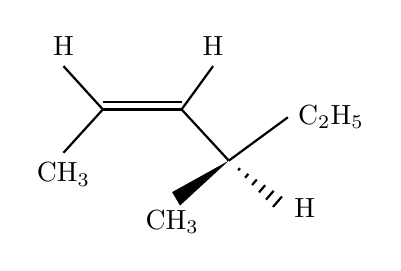
\begin{tikzpicture}[line width=.8pt]\draw(-2,0)--(-1,0);\draw(-2,.09)--(-1,.09);\draw(-2,0)--(-2.5,.55)node[above]{$\mathrm H$};\draw(-2,0)--(-2.5,-.55)node[below]{$\mathrm{CH_3}$};\draw(-1,0)--(-.6,.55)node[above]{$\mathrm H$};\draw(-1,0)--(-.4,-.65);\draw(-.4,-.65)--(.35,-.1)node[right]{$\mathrm{C_2H_5}$};\fill(-.4,-.65)--(-1.12,-1.05)--(-1.02,-1.22)--cycle;\node[below]at(-1.12,-1.15){$\mathrm{CH_3}$};\foreach \t in{.2,.35,.5,.65,.8,.95}{\draw({-.4+.65*\t-.06*\t},{-.65-.55*\t-.07*\t})--({-.4+.65*\t+.06*\t},{-.65-.55*\t+.07*\t});}\node[right]at(.3,-1.25){$\mathrm H$};\end{tikzpicture}\end{center}
\par\medskip\textbf{答案：}$(2Z,4R)$-4-甲基-2-己烯。
\textbf{推导与理由：}\begin{enumerate}\item 含双键最长主链6碳，从左侧烯端甲基编号使双键位于2；支链甲基在4。
\item 双键左端CH3优先H，右端手性碳优先H，两个高优先基团在同侧，故Z。
\item 手性中心四基团优先序：烯基＞乙基＞甲基＞H。烯基按重复原子规则在第一差异层高于乙基；H为虚楔指向纸后，1$\rightarrow$2$\rightarrow$3顺时针，故R。\end{enumerate}
\textbf{反向验算与边界：}\begin{itemize}\item 双键优先定位，不先给甲基低号；主链6碳加支链1碳总7碳；H背向已核，未无故再翻转。\end{itemize}
 原书答案对照：印刷125页。\par\medskip\clearpage\subsection*{6．（2分）}S02-M03-一-Q01\quad 印刷129页 / PDF138页。\par\bigskip
完成下列反应。
\begin{center}\begin{tabular}{ccc}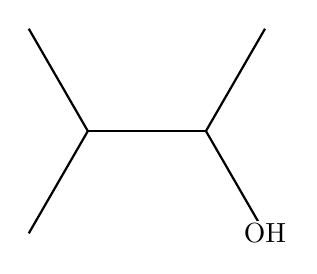
\begin{tikzpicture}[line width=.8pt]\draw (1.500,1.299)--(0.750,0.000);
\draw (0.750,0.000)--(1.500,-1.299);
\draw (0.750,0.000)--(-0.750,-0.000);
\draw (-0.750,-0.000)--(-1.500,-1.299);
\draw (-0.750,-0.000)--(-1.500,1.299);
\node[fill=white,inner sep=1.1pt]at(1.500,-1.299){$\mathrm{OH}$};\end{tikzpicture}&$\xrightarrow{\text{HCl}}$&（\qquad）\end{tabular}\end{center}
\par\medskip\textbf{答案：}主要重排取代产物为2-氯-2-甲基丁烷。
\begin{center}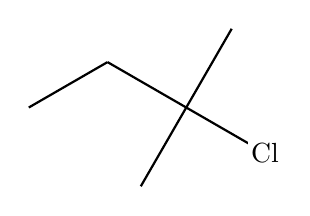
\begin{tikzpicture}[line width=.8pt]\draw (-1.500,0.000)--(-0.500,0.577);
\draw (-0.500,0.577)--(0.500,0.000);
\draw (0.500,0.000)--(-0.077,-1.000);
\draw (0.500,0.000)--(1.077,1.000);
\draw (0.500,0.000)--(1.500,-0.577);
\node[fill=white,inner sep=1.1pt]at(1.500,-0.577){$\mathrm{Cl}$};\end{tikzpicture}\end{center}
\textbf{推导与理由：}\begin{enumerate}\item 羟基被酸质子化，转成较好离去基团水；水离去可形成原羟基碳上的二级正离子。邻碳带H，1,2-氢迁移形成三级正离子，再由氯离子捕获。
\item 迁移的是带电子对的氢，正电移到原来的相邻碳。先将重排正离子全连接画出，再接Cl，不能只把Cl随意放到更拥挤位置。\end{enumerate}
\textbf{反向验算与边界：}\begin{itemize}\item 5碳骨架守恒；未重排的直接捕获可能并存，不宣称排他唯一；原书同样列重排三级氯代物为答案。\end{itemize}
 原书答案对照：印刷131页。\par\medskip\clearpage\subsection*{7．（2分）}S02-M03-一-Q02\quad 印刷129页 / PDF138页。\par\bigskip
完成下列反应。
\begin{center}\begin{tabular}{ccc}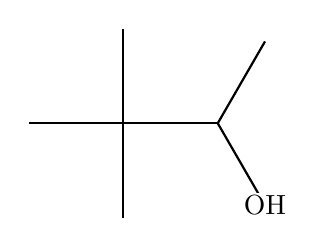
\begin{tikzpicture}[line width=.8pt]\draw (1.500,1.039)--(0.900,-0.000);
\draw (0.900,-0.000)--(1.500,-1.039);
\draw (0.900,-0.000)--(-0.300,-0.000);
\draw (-0.300,-0.000)--(-0.300,-1.200);
\draw (-0.300,-0.000)--(-0.300,1.200);
\draw (-0.300,-0.000)--(-1.500,0.000);
\node[fill=white,inner sep=1.1pt]at(1.500,-1.039){$\mathrm{OH}$};\end{tikzpicture}&$\xrightarrow{\text{浓硫酸，加热}}$&（\qquad）\end{tabular}\end{center}
\par\medskip\textbf{答案：}主要烯烃为2,3-二甲基-2-丁烯。
\begin{center}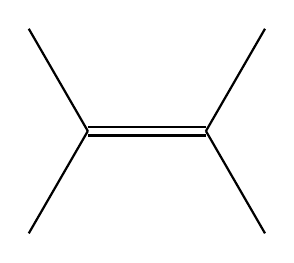
\begin{tikzpicture}[line width=.8pt]\draw (-1.500,1.299)--(-0.750,0.000);
\draw (-0.750,0.000)--(-1.500,-1.299);
\draw (-0.750,-0.055)--(0.750,-0.055);
\draw (-0.750,0.055)--(0.750,0.055);
\draw (0.750,-0.000)--(1.500,-1.299);
\draw (0.750,-0.000)--(1.500,1.299);\end{tikzpicture}\end{center}
\textbf{推导与理由：}\begin{enumerate}\item 羟基质子化离水后得到靠近季碳的二级正离子。邻季碳没有可迁移H，但可发生1,2-甲基迁移，得到更稳定的三级正离子。
\item 重排后从相邻碳失去$\beta$-H形成高度取代双键，得到四取代的2,3-二甲基-2-丁烯。
\item 直接消除及其他$\beta$位消除也存在机理分支，原书填空只给主要产物；此处不虚构各支路百分比。\end{enumerate}
\textbf{反向验算与边界：}\begin{itemize}\item 6碳守恒；迁移前季碳无H，不能写氢迁移；浓硫酸不是粗筛误写的稀硫酸。\end{itemize}
 原书答案对照：印刷131页。\par\medskip\clearpage\subsection*{8．（2分）}S02-M02-一-Q09\quad 印刷121页 / PDF130页。\par\bigskip
写出下列化合物的系统名称。
\begin{center}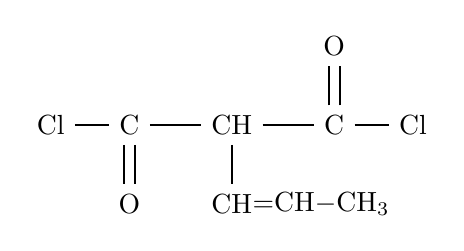
\begin{tikzpicture}[line width=.8pt]
\node(a)at(0,0){$\mathrm{Cl}$};\node(b)at(1,0){$\mathrm C$};\node(c)at(2.3,0){$\mathrm{CH}$};\node(d)at(3.6,0){$\mathrm C$};\node(e)at(4.6,0){$\mathrm{Cl}$};
\draw(a)--(b)--(c)--(d)--(e);\node(o1)at(1,-1){$\mathrm O$};\node(o2)at(3.6,1){$\mathrm O$};\draw([xshift=-2pt]b.south)--([xshift=-2pt]o1.north);\draw([xshift=2pt]b.south)--([xshift=2pt]o1.north);\draw([xshift=-2pt]d.north)--([xshift=-2pt]o2.south);\draw([xshift=2pt]d.north)--([xshift=2pt]o2.south);
\node(f)at(2.3,-1){$\mathrm{CH}$};\node[anchor=west,inner sep=0pt]at(2.55,-1){$\mathrm{{=}CH{-}CH_3}$};\draw(c)--(f);
\end{tikzpicture}\end{center}
\par\medskip\textbf{答案：}2-(丙-1-烯-1-基)丙二酰氯；按原书传统命名亦写2-氯甲酰基-3-戊烯酰氯。
\textbf{推导与理由：}\begin{enumerate}\item 先识别同一个CH上连接两个C(=O)Cl，为取代丙二酰氯。该CH连接的侧链为CH=CHCH3，即丙-1-烯-1-基，所以取代位在丙二酰氯的2位。
\item 若用旧式选择一条含酰氯和烯键的5碳主链命名，则另一酰氯作氯甲酰基在C2，双键在3，得到原书名称。两种表述必须对应同一连接图。\end{enumerate}
\textbf{反向验算与边界：}\begin{itemize}\item 两个酰氯均保留；不是氯代羧酸，也不是一个酯；6碳总数；原图未限定E/Z，不增造双键构型。\end{itemize}
 原书答案对照：印刷125页。\par 题源替换留痕：原条件NaOEt同时标E1消去与常规强碱E2相矛盾，按主线程要求换可靠原题，不在正式卷默改机理。\par\medskip\clearpage\subsection*{9．（2分）}S02-M03-一-Q08\quad 印刷129页 / PDF138页。\par\bigskip
完成下列反应，并画出产物稳定构象式。
\begin{center}\begin{tabular}{ccc}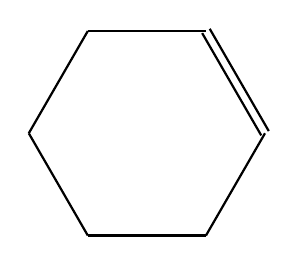
\begin{tikzpicture}[line width=.8pt]\draw (1.548,0.028)--(0.798,1.327);
\draw (1.452,-0.027)--(0.702,1.272);
\draw (0.750,1.299)--(-0.750,1.299);
\draw (-0.750,1.299)--(-1.500,0.000);
\draw (-1.500,0.000)--(-0.750,-1.299);
\draw (-0.750,-1.299)--(0.750,-1.299);
\draw (0.750,-1.299)--(1.500,0.000);\end{tikzpicture}&$\xrightarrow{\text{稀$\mathrm{KMnO_4}$溶液}}$&（\qquad）\end{tabular}\end{center}
\par\medskip\textbf{答案：}顺式环己烷-1,2-二醇，稳定椅式中一个OH为轴向、另一个为平伏，二者同面。
\begin{center}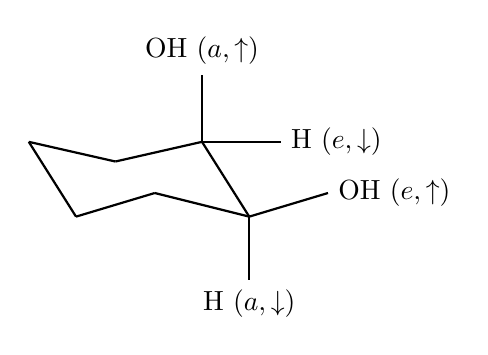
\begin{tikzpicture}[line width=.8pt]\draw(0.800,0.450)--(1.400,-0.500);
\draw(1.400,-0.500)--(0.200,-0.200);
\draw(0.200,-0.200)--(-0.800,-0.500);
\draw(-0.800,-0.500)--(-1.400,0.450);
\draw(-1.400,0.450)--(-0.300,0.200);
\draw(-0.300,0.200)--(0.800,0.450);
\draw(.8,.45)--(.8,1.3)node[above]{$\mathrm{OH}\ (a,\uparrow)$};
\draw(1.4,-.5)--(2.4,-.2)node[right]{$\mathrm{OH}\ (e,\uparrow)$};
\draw(1.4,-.5)--(1.4,-1.3)node[below]{$\mathrm H\ (a,\downarrow)$};
\draw(.8,.45)--(1.8,.45)node[right]{$\mathrm H\ (e,\downarrow)$};\end{tikzpicture}\end{center}
\textbf{推导与理由：}\begin{enumerate}\item 按本题稀高锰酸钾常规温和羟化语境，双键两个碳同面加入两个OH，得到顺1,2邻二醇。不能擅自升级为热浓条件的氧化裂解。
\item 在椅式环中相邻两个轴向交替上下。要使相邻OH同面，必须一轴一平伏；翻椅后两OH交换轴向和平伏，顺式关系不变。
\item 本题两个取代基相同，两个翻椅通常等能；题目要求画稳定构象，任一等效a/e椅式可。\end{enumerate}
\textbf{反向验算与边界：}\begin{itemize}\item 不是反式双平伏二醇；两OH同面，图上均向上；原题未给温度，不伪称原书有冷字；6碳环保留。\end{itemize}
 原书答案对照：印刷131页。\par\medskip\clearpage\subsection*{10．（2分）}原书：华东理工大学模拟试题（一） 一、回答问题 第4题；PDF[105]，印刷页[100]。\par\smallskip 命名\par\smallskip \par\smallskip \par\smallskip 用IUPAC命名下列化合物：\par\smallskip 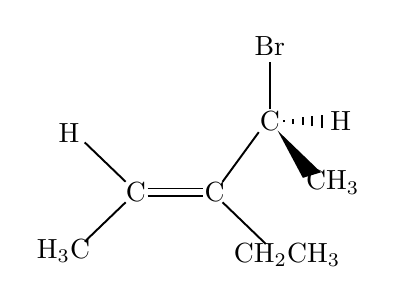
\begin{tikzpicture}[line width=.7pt]
\node at(-.7,0){C};\node at(.3,0){C};\draw(-.55,.045)--(.15,.045);\draw(-.55,-.045)--(.15,-.045);
\draw(-.83,.13)--(-1.35,.63);\node at(-1.55,.75){H};\draw(-.83,-.13)--(-1.35,-.63);\node at(-1.62,-.75){$\mathrm{H_3C}$};
\draw(.4,-.13)--(.95,-.66);\node at(1.22,-.8){$\mathrm{CH_2CH_3}$};\draw(.4,.13)--(.86,.76);\node at(1.,.9){C};\draw(1,1.05)--(1,1.65);\node at(1,1.85){Br};
\fill(1.1,.78)--(1.65,.25)--(1.42,.18)--cycle;\node at(1.8,.12){$\mathrm{CH_3}$};
\foreach \x in {1.18,1.3,1.42,1.54,1.66}{\draw(\x,{.9-0.15*(\x-1.1)})--(\x,{.9+0.15*(\x-1.1)});}\node at(1.9,.9){H};
\end{tikzpicture}\par\smallskip \par\smallskip \textbf{答案（顺原空次序）：}\par\smallskip \par\smallskip (2E,4S)-4-溴-3-乙基戊-2-烯。\par\smallskip \par\smallskip \textbf{推导：}最长含双键链是戊-2-烯，选经含Br手性碳的主链可使取代信息完整，支链为3-乙基、4-溴。烯键左端Me优于H；右端CH(Br)Me的下一层Br优于乙基的H/C，因此两高优先基团在相反侧，为2E。C4优先级Br>烯基>Me>H；H虚键背向，1→2→3逆时针，为4S。\par\smallskip \par\smallskip \textbf{反校：}不以“体积大”替代CIP原子序数；右端优先级不是只看两者直接相连都为C就停；H背向再读手性。\par\smallskip \par\smallskip \textbf{2分参考采分：}母体及取代位1分；E与S各0.5分。\par\smallskip \par\smallskip 独立推导后对照本书参考答案PDF110页；有原答案缺笔处以原题碳骨架/反应守恒校正，不盲抄。\par\smallskip \par\medskip\clearpage\subsection*{11．（2分）}原书：华东理工大学模拟试题（一） 一、回答问题 第33题；PDF[108]，印刷页[103]。\par\smallskip 完成反应，填写全部原空\par\smallskip \par\smallskip 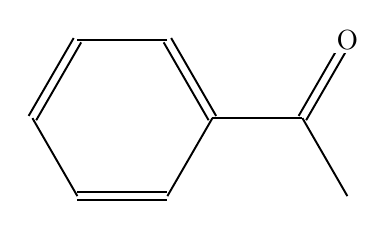
\begin{tikzpicture}[line width=.7pt]\draw (2.000,-0.990)--(1.429,0.000);
\draw (1.476,-0.027)--(2.048,0.962);
\draw (1.381,0.028)--(1.952,1.017);
\draw (1.429,0.000)--(0.286,0.000);
\draw (0.333,0.028)--(-0.238,1.017);
\draw (0.238,-0.027)--(-0.333,0.962);
\draw (-0.286,0.990)--(-1.429,0.990);
\draw (-1.476,1.017)--(-2.048,0.028);
\draw (-1.381,0.962)--(-1.952,-0.027);
\draw (-2.000,0.000)--(-1.429,-0.990);
\draw (-1.429,-1.045)--(-0.286,-1.045);
\draw (-1.429,-0.935)--(-0.286,-0.935);
\draw (-0.286,-0.990)--(0.286,0.000);
\node[fill=white,inner sep=1.1pt]at(2.000,0.990){$\mathrm{O}$};\end{tikzpicture}$+$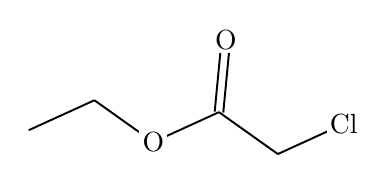
\begin{tikzpicture}[line width=.7pt]\draw (-2.000,-0.421)--(-1.165,-0.040);
\draw (-1.165,-0.040)--(-0.417,-0.572);
\draw (-0.417,-0.572)--(0.417,-0.191);
\draw (0.472,-0.196)--(0.559,0.718);
\draw (0.363,-0.185)--(0.450,0.728);
\draw (0.417,-0.191)--(1.165,-0.723);
\draw (1.165,-0.723)--(2.000,-0.342);
\node[fill=white,inner sep=1.1pt]at(-0.417,-0.572){$\mathrm{O}$};
\node[fill=white,inner sep=1.1pt]at(0.505,0.723){$\mathrm{O}$};
\node[fill=white,inner sep=1.1pt]at(2.000,-0.342){$\mathrm{Cl}$};\end{tikzpicture}$\xrightarrow{\ EtONa\ }$（空1）$\xrightarrow{\ 1.OH^-;2.H^+,\Delta\ }$（空2）\par\smallskip \par\smallskip \textbf{答案（顺原空次序）：}\par\smallskip \begin{minipage}[c]{.48\linewidth}\centering (1)\par \scalebox{.83}{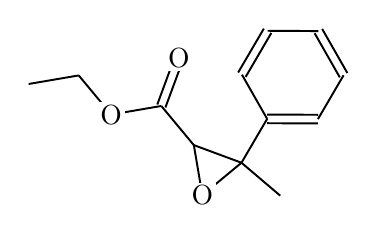
\begin{tikzpicture}[line width=.7pt]\draw (-2.000,0.371)--(-1.364,0.480);
\draw (-1.364,0.480)--(-0.951,-0.017);
\draw (-0.951,-0.017)--(-0.315,0.092);
\draw (-0.263,0.073)--(-0.039,0.678);
\draw (-0.366,0.111)--(-0.143,0.716);
\draw (-0.315,0.092)--(0.098,-0.405);
\draw (0.098,-0.405)--(0.206,-1.041);
\draw (0.206,-1.041)--(0.703,-0.629);
\draw (0.703,-0.629)--(1.195,-1.047);
\draw (0.703,-0.629)--(1.029,-0.072);
\draw (1.028,-0.127)--(1.674,-0.130);
\draw (1.029,-0.017)--(1.675,-0.020);
\draw (1.674,-0.075)--(2.000,0.482);
\draw (2.048,0.510)--(1.728,1.070);
\draw (1.952,0.455)--(1.632,1.016);
\draw (1.680,1.043)--(1.035,1.047);
\draw (0.987,1.074)--(0.661,0.517);
\draw (1.082,1.019)--(0.756,0.461);
\draw (0.703,-0.629)--(0.098,-0.405);
\draw (0.709,0.489)--(1.029,-0.072);
\node[fill=white,inner sep=1.1pt]at(-0.951,-0.017){$\mathrm{O}$};
\node[fill=white,inner sep=1.1pt]at(-0.091,0.697){$\mathrm{O}$};
\node[fill=white,inner sep=1.1pt]at(0.206,-1.041){$\mathrm{O}$};\end{tikzpicture}}\end{minipage}\begin{minipage}[c]{.48\linewidth}\centering (2)\par \scalebox{.83}{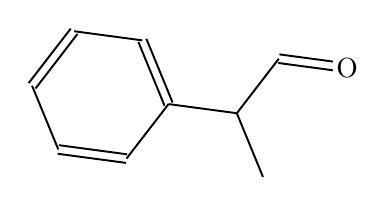
\begin{tikzpicture}[line width=.7pt]\draw (0.932,-0.925)--(0.600,-0.116);
\draw (0.600,-0.116)--(1.133,0.576);
\draw (1.126,0.522)--(1.993,0.406);
\draw (1.141,0.631)--(2.007,0.515);
\draw (0.600,-0.116)--(-0.267,-0.000);
\draw (-0.216,0.021)--(-0.549,0.829);
\draw (-0.318,-0.021)--(-0.650,0.788);
\draw (-0.600,0.809)--(-1.466,0.925);
\draw (-1.510,0.958)--(-2.044,0.266);
\draw (-1.423,0.891)--(-1.956,0.199);
\draw (-2.000,0.232)--(-1.667,-0.576);
\draw (-1.675,-0.631)--(-0.808,-0.747);
\draw (-1.660,-0.522)--(-0.793,-0.638);
\draw (-0.801,-0.692)--(-0.267,-0.000);
\node[fill=white,inner sep=1.1pt]at(2.000,0.460){$\mathrm{O}$};\end{tikzpicture}}\end{minipage}\par\medskip\par\smallskip \textbf{推导：}$\alpha$氯代酯去质子化后进攻苯乙酮，再由所得烷氧负离子分子内取代Cl闭合成环氧酯，这是Darzens缩合。水解酯并脱羧时环氧羧酸发生重排，得到碳骨架延长一个碳的2-苯基丙醛。醛的羰基碳来自氯代酯$\alpha$碳，而非原苯乙酮羰基。\par\smallskip \par\smallskip \textbf{反校：}环氧三角含一个O；原酮碳保留Ph与Me，不能丢Me；末产物为PhCH(Me)CHO而非PhCH2COCH3。\par\smallskip \par\smallskip \textbf{2分参考采分：}环氧酯1分；2-苯基丙醛1分。\par\smallskip \par\smallskip \textbf{边界/原印问题：}原料未给手性，环氧酯相对构型未指定；不编单一异构体，末端醛按外消旋/未指定构型表达。\par\smallskip \par\smallskip 独立推导后对照本书参考答案PDF111页；有原答案缺笔处以原题碳骨架/反应守恒校正，不盲抄。\par\smallskip \par\medskip\clearpage\subsection*{12．（2分）}原书：华东理工大学模拟试题（一） 一、回答问题 第35题；PDF[108]，印刷页[103]。\par\smallskip 完成反应，填写全部原空\par\smallskip \par\smallskip 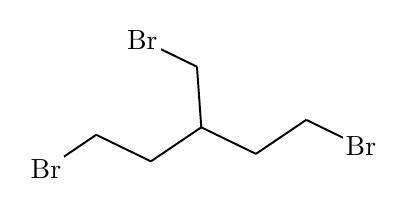
\begin{tikzpicture}[line width=.7pt]\draw (2.000,-0.532)--(1.306,-0.195);
\draw (1.306,-0.195)--(0.667,-0.627);
\draw (0.667,-0.627)--(-0.027,-0.290);
\draw (-0.027,-0.290)--(-0.667,-0.722);
\draw (-0.667,-0.722)--(-1.361,-0.385);
\draw (-1.361,-0.385)--(-2.000,-0.817);
\draw (-0.027,-0.290)--(-0.082,0.480);
\draw (-0.082,0.480)--(-0.777,0.817);
\node[fill=white,inner sep=1.1pt]at(2.000,-0.532){$\mathrm{Br}$};
\node[fill=white,inner sep=1.1pt]at(-2.000,-0.817){$\mathrm{Br}$};
\node[fill=white,inner sep=1.1pt]at(-0.777,0.817){$\mathrm{Br}$};\end{tikzpicture}$+\mathrm{NH_3}$$\xrightarrow{\ \ }$（空）\par\smallskip \par\smallskip \textbf{答案（顺原空次序）：}\par\smallskip \par\medskip 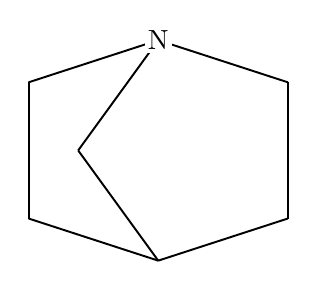
\begin{tikzpicture}[line width=.7pt]\draw (1.646,-0.865)--(1.646,0.865);
\draw (1.646,0.865)--(0.000,1.400);
\draw (0.000,1.400)--(-1.646,0.865);
\draw (-1.646,0.865)--(-1.646,-0.865);
\draw (-1.646,-0.865)--(-0.000,-1.400);
\draw (-0.000,-1.400)--(-1.017,0.000);
\draw (-0.000,-1.400)--(1.646,-0.865);
\draw (-1.017,0.000)--(0.000,1.400);
\node[fill=white,inner sep=1.1pt]at(0.000,1.400){$\mathrm{N}$};\end{tikzpicture}\par\medskip\par\smallskip \textbf{推导：}三条末端一级溴代链分别是两条—CH2CH2Br和一条—CH2Br，都连在同一个中心CH。氨先作一次取代，氮再对另外两条末端C—Br发生分子内取代，三次成键后成为三级桥头氮。以原中心碳和氮作两个桥头，三条桥内原子数为2、2、1，得到1-氮杂双环[2.2.1]庚烷。\par\smallskip \par\smallskip \textbf{反校：}底物6C，产物仍6C加1N；桥头N共有三根C—N键无N—H；三条桥长度不能全部画成2（那将错成奎宁环）。\par\smallskip \par\smallskip \textbf{2分参考采分：}两个桥头与[2.2.1]连接1分；N位置/三键与6C正确1分。\par\smallskip \par\smallskip \textbf{边界/原印问题：}原题没有浓度/当量，按其预期分子内成环主要结构作答，不将此教材结构推导冒称定量或唯一实验产物；实际聚合竞争需条件优化。原参考答案桥头N字样不清，不能据此把含氮题画成纯烃。\par\smallskip \par\smallskip 独立推导后对照本书参考答案PDF111页；有原答案缺笔处以原题碳骨架/反应守恒校正，不盲抄。\par\smallskip \par\medskip\clearpage\subsection*{13．（2分）}原书：复旦大学模拟试题（三） 二、完成反应 第13题；PDF[156]，印刷页[151]。\par\smallskip 完成反应，填写全部原空\par\smallskip \par\smallskip 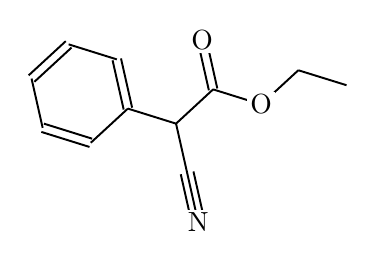
\begin{tikzpicture}[line width=.7pt]\draw (2.000,0.583)--(1.388,0.773);
\draw (1.388,0.773)--(0.917,0.339);
\draw (0.917,0.339)--(0.306,0.530);
\draw (0.359,0.542)--(0.219,1.167);
\draw (0.252,0.518)--(0.111,1.143);
\draw (0.306,0.530)--(-0.165,0.095);
\draw (-0.165,0.095)--(-0.024,-0.530);
\draw (-0.105,-0.548)--(0.036,-1.173);
\draw (-0.024,-0.530)--(0.116,-1.155);
\draw (0.056,-0.512)--(0.197,-1.137);
\draw (-0.165,0.095)--(-0.777,0.286);
\draw (-0.723,0.298)--(-0.864,0.923);
\draw (-0.830,0.274)--(-0.971,0.899);
\draw (-0.917,0.911)--(-1.529,1.102);
\draw (-1.566,1.142)--(-2.037,0.708);
\draw (-1.492,1.061)--(-1.963,0.627);
\draw (-2.000,0.667)--(-1.859,0.042);
\draw (-1.876,-0.010)--(-1.264,-0.201);
\draw (-1.843,0.095)--(-1.231,-0.096);
\draw (-1.248,-0.148)--(-0.777,0.286);
\node[fill=white,inner sep=1.1pt]at(0.917,0.339){$\mathrm{O}$};
\node[fill=white,inner sep=1.1pt]at(0.165,1.155){$\mathrm{O}$};
\node[fill=white,inner sep=1.1pt]at(0.116,-1.155){$\mathrm{N}$};\end{tikzpicture}$+$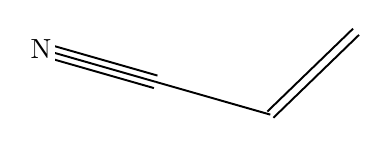
\begin{tikzpicture}[line width=.7pt]\draw (1.962,0.566)--(0.873,-0.487);
\draw (2.038,0.487)--(0.950,-0.566);
\draw (0.911,-0.526)--(-0.544,-0.110);
\draw (-0.522,-0.030)--(-1.977,0.386);
\draw (-0.544,-0.110)--(-2.000,0.307);
\draw (-0.567,-0.189)--(-2.023,0.228);
\node[fill=white,inner sep=1.1pt]at(-2.000,0.307){$\mathrm{N}$};\end{tikzpicture}$\xrightarrow{\ KOH/t\!\!-BuOK\ }$（空）\par\smallskip \par\smallskip \textbf{答案（顺原空次序）：}\par\smallskip \par\medskip 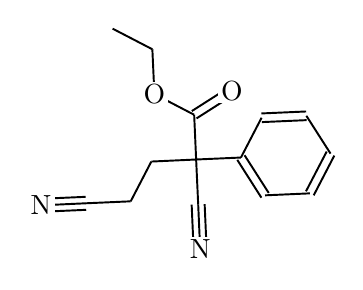
\begin{tikzpicture}[line width=.7pt]\draw (-0.930,1.400)--(-0.425,1.138);
\draw (-0.425,1.138)--(-0.399,0.569);
\draw (-0.399,0.569)--(0.106,0.306);
\draw (0.136,0.260)--(0.615,0.566);
\draw (0.076,0.353)--(0.556,0.659);
\draw (0.106,0.306)--(0.131,-0.262);
\draw (0.131,-0.262)--(0.157,-0.831);
\draw (0.074,-0.835)--(0.099,-1.404);
\draw (0.157,-0.831)--(0.182,-1.400);
\draw (0.239,-0.828)--(0.264,-1.396);
\draw (0.131,-0.262)--(-0.438,-0.288);
\draw (-0.438,-0.288)--(-0.700,-0.793);
\draw (-0.700,-0.793)--(-1.269,-0.818);
\draw (-1.272,-0.736)--(-1.841,-0.761);
\draw (-1.269,-0.818)--(-1.838,-0.844);
\draw (-1.265,-0.901)--(-1.834,-0.926);
\draw (0.131,-0.262)--(0.700,-0.237);
\draw (0.654,-0.267)--(0.960,-0.747);
\draw (0.746,-0.208)--(1.053,-0.687);
\draw (1.006,-0.717)--(1.575,-0.692);
\draw (1.624,-0.717)--(1.886,-0.212);
\draw (1.526,-0.666)--(1.789,-0.161);
\draw (1.838,-0.187)--(1.531,0.293);
\draw (1.529,0.348)--(0.960,0.323);
\draw (1.534,0.238)--(0.965,0.213);
\draw (0.962,0.268)--(0.700,-0.237);
\node[fill=white,inner sep=1.1pt]at(-0.399,0.569){$\mathrm{O}$};
\node[fill=white,inner sep=1.1pt]at(0.586,0.613){$\mathrm{O}$};
\node[fill=white,inner sep=1.1pt]at(0.182,-1.400){$\mathrm{N}$};
\node[fill=white,inner sep=1.1pt]at(-1.838,-0.844){$\mathrm{N}$};\end{tikzpicture}\par\medskip\par\smallskip \textbf{推导：}氰基与酯羰基共同稳定$\alpha$碳负离子。该位唯一的H被碱移去后，碳亲核端进攻丙烯腈$\beta$碳，形成Michael的1,4-加成；再质子化生成—CH2CH2CN支链。原Ph、CN和CO2Et都仍连接在同一四取代碳。\par\smallskip \par\smallskip \textbf{反校：}反应物11C+丙烯腈3C=14C；产物有两个CN；不能对腈碳作1,2加成，也不能无条件水解酯。\par\smallskip \par\smallskip \textbf{2分参考采分：}四取代中心保留Ph/CN/CO2Et1分；新—CH2CH2CN支链1分。\par\smallskip \par\smallskip \textbf{边界/原印问题：}原箭头上下印KOH和t-BuOK，原样保留；不据模糊简写改成另一结构。\par\smallskip \par\smallskip 独立推导后对照本书参考答案PDF158页；有原答案缺笔处以原题碳骨架/反应守恒校正，不盲抄。\par\smallskip \par\medskip\clearpage\subsection*{14．（2分）}原书：上海大学模拟试题（一） 二、完成反应 第7题；PDF[200]，印刷页[195]。\par\smallskip 完成反应，填写全部原空\par\smallskip \par\smallskip 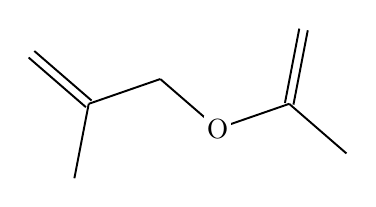
\begin{tikzpicture}[line width=.7pt]\draw (-2.036,0.588)--(-1.309,-0.042);
\draw (-1.964,0.671)--(-1.237,0.042);
\draw (-1.273,-0.000)--(-1.455,-0.945);
\draw (-1.273,-0.000)--(-0.364,0.315);
\draw (-0.364,0.315)--(0.364,-0.315);
\draw (0.364,-0.315)--(1.273,-0.000);
\draw (1.273,-0.000)--(2.000,-0.630);
\draw (1.327,-0.010)--(1.509,0.934);
\draw (1.219,0.010)--(1.401,0.955);
\node[fill=white,inner sep=1.1pt]at(0.364,-0.315){$\mathrm{O}$};\end{tikzpicture}$\xrightarrow{\ \Delta\ }$（空）\par\smallskip \par\smallskip \textbf{答案（顺原空次序）：}\par\smallskip \par\medskip 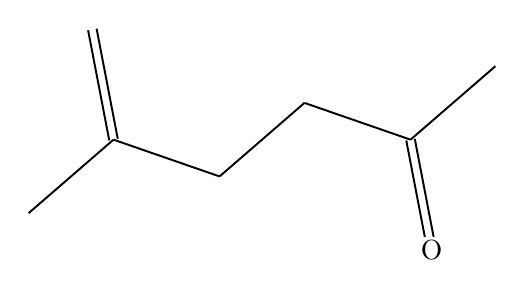
\begin{tikzpicture}[line width=.7pt]\draw (2.964,0.933)--(1.886,-0.000);
\draw (1.832,-0.010)--(2.101,-1.410);
\draw (1.940,0.010)--(2.209,-1.390);
\draw (1.886,-0.000)--(0.539,0.467);
\draw (0.539,0.467)--(-0.539,-0.467);
\draw (-0.539,-0.467)--(-1.886,-0.000);
\draw (-1.886,-0.000)--(-2.964,-0.933);
\draw (-1.832,0.010)--(-2.101,1.410);
\draw (-1.940,-0.010)--(-2.209,1.390);
\node[fill=white,inner sep=1.1pt]at(2.155,-1.400){$\mathrm{O}$};\end{tikzpicture}\par\medskip\par\smallskip \textbf{推导：}将底物按O—烯基端与O—烯丙基端分开，找出六原子重排路径。Claisen[3,3]重排断开O—烯丙基首碳键，并把两端的末端碳相连；O所连烯基碳变成羰基。得到CH3COCH2CH2C(CH3)=CH2，即5-甲基己-5-烯-2-酮。\par\smallskip \par\smallskip \textbf{反校：}起料7C+1O全部保留；新双键在末端且带甲基；不能只把O断开后拼成直链不同异构体。\par\smallskip \par\smallskip \textbf{2分参考采分：}羰基位置和7C骨架1分；新键及末端异丙烯基正确1分。\par\smallskip \par\smallskip 独立推导后对照本书参考答案PDF203页；有原答案缺笔处以原题碳骨架/反应守恒校正，不盲抄。\par\smallskip \par\medskip\clearpage\subsection*{15．（2分）}原书：上海大学模拟试题（二） 二、完成反应 第3题；PDF[209]，印刷页[204]。\par\smallskip 完成反应，填写全部原空\par\smallskip \par\smallskip $\mathrm{HC\equiv CH}$$\xrightarrow{\ NaNH_2/NH_3(l)\ }$（空1）$\xrightarrow{\ CH_3I\ }$（空2）$\xrightarrow{\ NaNH_2/NH_3(l)\ }$（空3）\par\smallskip 再与丙酮反应，生成（空4）：\par\smallskip \begin{tikzpicture}[line width=.7pt]\draw (-1.617,-1.400)--(0.000,-0.467);
\draw (0.055,-0.467)--(0.055,1.400);
\draw (-0.055,-0.467)--(-0.055,1.400);
\draw (0.000,-0.467)--(1.617,-1.400);
\node[fill=white,inner sep=1.1pt]at(0.000,1.400){$\mathrm{O}$};\end{tikzpicture}\par\smallskip \par\smallskip \textbf{答案（顺原空次序）：}\par\smallskip \begin{minipage}[c]{.32\linewidth}\centering (1)\par \scalebox{.83}{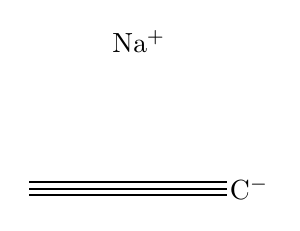
\begin{tikzpicture}[line width=.7pt]\draw (1.400,-0.851)--(-1.400,-0.851);
\draw (1.400,-0.933)--(-1.400,-0.933);
\draw (1.400,-1.016)--(-1.400,-1.016);
\node[fill=white,inner sep=1.1pt]at(0.000,0.933){$\mathrm{Na^{+}}$};
\node[fill=white,inner sep=1.1pt]at(1.400,-0.933){$\mathrm{C^{-}}$};\end{tikzpicture}}\end{minipage}\begin{minipage}[c]{.32\linewidth}\centering (2)\par \scalebox{.83}{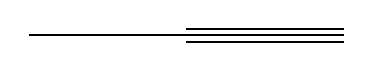
\begin{tikzpicture}[line width=.7pt]\draw (-2.000,0.000)--(-0.000,-0.000);
\draw (-0.000,-0.083)--(2.000,-0.083);
\draw (-0.000,-0.000)--(2.000,-0.000);
\draw (-0.000,0.082)--(2.000,0.082);\end{tikzpicture}}\end{minipage}\begin{minipage}[c]{.32\linewidth}\centering (3)\par \scalebox{.83}{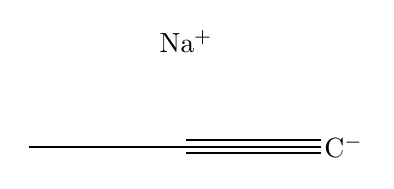
\begin{tikzpicture}[line width=.7pt]\draw (2.000,-0.584)--(0.000,-0.584);
\draw (2.000,-0.667)--(0.000,-0.667);
\draw (2.000,-0.749)--(0.000,-0.749);
\draw (0.000,-0.667)--(-2.000,-0.667);
\node[fill=white,inner sep=1.1pt]at(0.000,0.667){$\mathrm{Na^{+}}$};
\node[fill=white,inner sep=1.1pt]at(2.000,-0.667){$\mathrm{C^{-}}$};\end{tikzpicture}}\end{minipage}\par\medskip\begin{minipage}[c]{.32\linewidth}\centering (4)\par \scalebox{.83}{\begin{tikzpicture}[line width=.7pt]\draw (-2.000,0.000)--(-1.000,0.000);
\draw (-1.000,-0.083)--(-0.000,-0.083);
\draw (-1.000,0.000)--(-0.000,0.000);
\draw (-1.000,0.083)--(-0.000,0.083);
\draw (-0.000,0.000)--(1.000,0.000);
\draw (1.000,0.000)--(1.000,1.000);
\draw (1.000,0.000)--(1.000,-1.000);
\draw (1.000,0.000)--(2.000,0.000);
\node[fill=white,inner sep=1.1pt]at(2.000,0.000){$\mathrm{OH}$};\end{tikzpicture}}\end{minipage}\par\medskip\par\smallskip \textbf{推导：}NaNH2先脱去端炔氢，乙炔负离子对CH3I发生一级SN2形成丙炔。丙炔尚有一个端炔氢，再被NaNH2夺取，所得丙炔负离子加成丙酮羰基；水后处理形成三级炔丙醇CH3C$\equiv$CC(OH)(CH3)2。\par\smallskip \par\smallskip \textbf{反校：}第二空为丙炔而不是2-丁炔；第三空仍应有Na和负电荷；最终3C+丙酮3C=6C，OH碳无H。\par\smallskip \par\smallskip \textbf{2分参考采分：}四个连续空各0.5分，共2分，不删空。\par\smallskip \par\smallskip \textbf{边界/原印问题：}原末箭头未另印H2O，原书答案按通常水后处理写醇；教师解说水处理前为烷氧钠，接受该明确中间形式。\par\smallskip \par\smallskip 独立推导后对照本书参考答案PDF211页；有原答案缺笔处以原题碳骨架/反应守恒校正，不盲抄。\par\smallskip \par\medskip\clearpage\clearpage\section*{二、选择题（12题，共12分）}\subsection*{1．（1分）}\textbf{参考答案：D}\par\medskip{}模拟试题1·一·3\quad 印刷115页 / PDF 124页
\par\bigskip
下列哪种卤代烃发生$\mathrm{E2}$过程的反应速率最大（\quad），原因是（\qquad）。
\par\bigskip
\begin{minipage}[t]{.48\linewidth}\vspace{0pt}\textbf{(A)}\par\smallskip 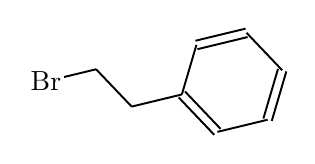
\begin{tikzpicture}[line width=.7pt,>=Stealth]
\draw (-1.500,0.012)--(-0.863,0.166);
\draw (-0.863,0.166)--(-0.411,-0.308);
\draw (-0.411,-0.308)--(0.226,-0.154);
\draw (0.186,-0.192)--(0.638,-0.667);
\draw (0.266,-0.116)--(0.718,-0.591);
\draw (0.678,-0.629)--(1.315,-0.475);
\draw (1.368,-0.490)--(1.553,0.139);
\draw (1.262,-0.459)--(1.447,0.170);
\draw (1.500,0.154)--(1.048,0.629);
\draw (1.035,0.682)--(0.398,0.528);
\draw (1.061,0.575)--(0.424,0.421);
\draw (0.411,0.475)--(0.226,-0.154);
\node[fill=white,inner sep=1.1pt]at(-1.500,0.012){$\mathrm{Br}$};
\end{tikzpicture}\end{minipage}\hfill
\begin{minipage}[t]{.48\linewidth}\vspace{0pt}\textbf{(B)}\par\smallskip $p$-$\mathrm{CH_3C_6H_4CH_2CH_2Br}$\end{minipage}\par\bigskip
\begin{minipage}[t]{.48\linewidth}\vspace{0pt}\textbf{(C)}\par\smallskip $p$-$\mathrm{ClC_6H_4CH_2CH_2Br}$\end{minipage}\hfill
\begin{minipage}[t]{.48\linewidth}\vspace{0pt}\textbf{(D)}\par\smallskip $p$-$\mathrm{NO_2C_6H_4CH_2CH_2Br}$\end{minipage}\par\bigskip
\par\bigskip\textbf{教师答案：}D
\par\medskip\textbf{从依据到结论：}E2中碱取走$\beta$-H，同时成双键并离去Br。此系列$\beta$位即苄位，过渡态中发展的负电荷性质可由吸电子取代基稳定。对硝基的吸电子作用最强，使苄位氢更易被碱夺取，所以D最快。
\par\medskip\textbf{选项排除：}B对甲基给电子，不利这一取氢趋势；A无硝基稳定；C有吸电子作用但通常弱于对硝基。
\par\medskip\textbf{反向核对及边界：}不拿苄基正离子稳定性解释本题；原底物离去基位于末端，不是直接连苯环的芳基溴。速率比较限同一E2条件。
\par\smallskip 本书对照：印刷118页，原答案D；NO2使苯环$\alpha$-H酸性增加。
\par\medskip\clearpage\subsection*{2．（1分）}\textbf{参考答案：D}\par\medskip{}模拟试题4·一·3\quad 印刷135页 / PDF 144页
\par\bigskip
下列共振结构式中（\quad）共振结构对共振杂化体的贡献最大。
\par\bigskip
\begin{minipage}[t]{.48\linewidth}\vspace{0pt}\textbf{(A)}\par\smallskip 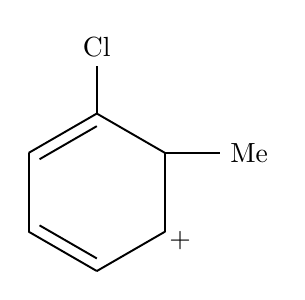
\begin{tikzpicture}[line width=.7pt,>=Stealth]
\draw(0,1)--(0.866,0.5);
\draw(0.866,0.5)--(0.866,-0.5);
\draw(0.866,-0.5)--(0,-1);
\draw(0,-1)--(-0.866,-0.5);
\draw(0.0,-0.84)--(-0.72744,-0.42);
\draw(-0.866,-0.5)--(-0.866,0.5);
\draw(-0.866,0.5)--(0,1);
\draw(-0.72744,0.42)--(0.0,0.84);
\draw(0,1)--(0,1.6)node[above]{$\mathrm{Cl}$};
\draw(0.866,0.5)--(1.5659999999999998,0.5)node[right]{$\mathrm{Me}$};
\node at(1.05652,-0.61){$+$};
\end{tikzpicture}\end{minipage}\hfill
\begin{minipage}[t]{.48\linewidth}\vspace{0pt}\textbf{(B)}\par\smallskip 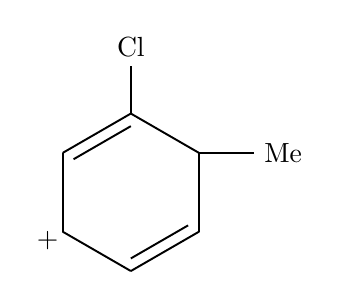
\begin{tikzpicture}[line width=.7pt,>=Stealth]
\draw(0,1)--(0.866,0.5);
\draw(0.866,0.5)--(0.866,-0.5);
\draw(0.866,-0.5)--(0,-1);
\draw(0.72744,-0.42)--(0.0,-0.84);
\draw(0,-1)--(-0.866,-0.5);
\draw(-0.866,-0.5)--(-0.866,0.5);
\draw(-0.866,0.5)--(0,1);
\draw(-0.72744,0.42)--(0.0,0.84);
\draw(0,1)--(0,1.6)node[above]{$\mathrm{Cl}$};
\draw(0.866,0.5)--(1.5659999999999998,0.5)node[right]{$\mathrm{Me}$};
\node at(-1.05652,-0.61){$+$};
\end{tikzpicture}\end{minipage}\par\bigskip
\begin{minipage}[t]{.48\linewidth}\vspace{0pt}\textbf{(C)}\par\smallskip 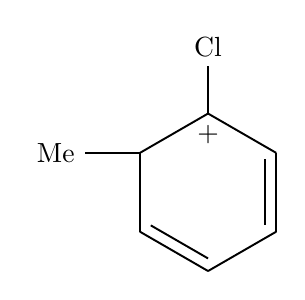
\begin{tikzpicture}[line width=.7pt,>=Stealth]
\draw(0,1)--(0.866,0.5);
\draw(0.866,0.5)--(0.866,-0.5);
\draw(0.72744,0.42)--(0.72744,-0.42);
\draw(0.866,-0.5)--(0,-1);
\draw(0,-1)--(-0.866,-0.5);
\draw(0.0,-0.84)--(-0.72744,-0.42);
\draw(-0.866,-0.5)--(-0.866,0.5);
\draw(-0.866,0.5)--(0,1);
\draw(0,1)--(0,1.6)node[above]{$\mathrm{Cl}$};
\draw(-0.866,0.5)--(-1.5659999999999998,0.5)node[left]{$\mathrm{Me}$};
\node at(0,0.73){$+$};
\end{tikzpicture}\end{minipage}\hfill
\begin{minipage}[t]{.48\linewidth}\vspace{0pt}\textbf{(D)}\par\smallskip 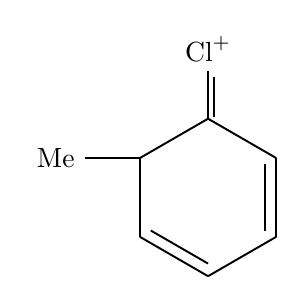
\begin{tikzpicture}[line width=.7pt,>=Stealth]
\draw(0,1)--(0.866,0.5);
\draw(0.866,0.5)--(0.866,-0.5);
\draw(0.72744,0.42)--(0.72744,-0.42);
\draw(0.866,-0.5)--(0,-1);
\draw(0,-1)--(-0.866,-0.5);
\draw(0.0,-0.84)--(-0.72744,-0.42);
\draw(-0.866,-0.5)--(-0.866,0.5);
\draw(-0.866,0.5)--(0,1);
\draw(0,1)--(0,1.6)node[above]{$\mathrm{Cl}^{+}$};
\draw(.07,1.02)--(.07,1.53);
\draw(-0.866,0.5)--(-1.5659999999999998,0.5)node[left]{$\mathrm{Me}$};
\end{tikzpicture}\end{minipage}\par\bigskip
\par\bigskip\textbf{教师答案：}D
\par\medskip\textbf{从依据到结论：}共振式原子位置相同，仅电子移动。评估贡献先查八隅体，再查电荷。D以氯孤对供电子形成C=Cl的带正电贡献式，使相关碳补足八电子；与存在缺电子碳的贡献式相比，这一八隅体优势是主要判断依据。
\par\medskip\textbf{选项排除：}A、B、C仍含六电子碳正离子；不能只因正电荷在电负性较大的氯上就机械排除D。
\par\medskip\textbf{反向核对及边界：}逐原子复查总正电荷相同、氯与甲基连接位置对应同一骨架，双键移动而$\sigma$骨架未变。
\par\smallskip 本书对照：印刷137页，原答案D。
\par\medskip\clearpage\subsection*{3．（1分）}\textbf{参考答案：A}\par\medskip{}模拟试题4·一·5\quad 印刷135页 / PDF 144页
\par\bigskip
下列反应应该选择（\quad）作为氧化剂。
\par\bigskip
\begin{center}\[\begin{array}{c}\mathrm{C_6H_5{-}CH{=}CH{-}\underset{\displaystyle |\atop\mathrm{CH_3}}{CH}{-}OH}\end{array}\ \longrightarrow\ \mathrm{C_6H_5{-}CH{=}CH{-}C(=O){-}OH}\]\end{center}
\begin{minipage}[t]{.48\linewidth}\vspace{0pt}\textbf{(A)}\par\smallskip $\mathrm{I_2/NaOH}$\end{minipage}\hfill
\begin{minipage}[t]{.48\linewidth}\vspace{0pt}\textbf{(B)}\par\smallskip $\mathrm{O_3}$\end{minipage}\par\bigskip
\begin{minipage}[t]{.48\linewidth}\vspace{0pt}\textbf{(C)}\par\smallskip $\mathrm{KMnO_4}$\end{minipage}\hfill
\begin{minipage}[t]{.48\linewidth}\vspace{0pt}\textbf{(D)}\par\smallskip $\mathrm{HNO_3}$\end{minipage}\par\bigskip
\par\bigskip\textbf{教师答案：}A
\par\medskip\textbf{从依据到结论：}先将仲醇氧化为甲基酮PhCH=CHCOCH3，再由I2/NaOH连续碘化该甲基，经亲核酰基取代裂解为肉桂酸根和CHI3。通常酸化分离后得到原图游离肉桂酸。
\par\medskip\textbf{选项排除：}B臭氧主要断双键；C高锰酸钾易同时进攻所需保留的C=C；D硝酸不是这里针对甲基酮侧链的选择性碘仿试剂。
\par\medskip\textbf{反向核对及边界：}原选项只写I2/NaOH，不暗加酸化为原印刷条件：严格碱性反应液产物是盐，游离酸是后处理形式。核10碳底物$\rightarrow$9碳酸/盐+1碳CHI3，双键保留。
\par\smallskip 本书对照：印刷137页，原答案A。
\par\medskip\clearpage\subsection*{4．（1分）}\textbf{参考答案：D}\par\medskip{}模拟试题8·一·10\quad 印刷159页 / PDF 168页
\par\bigskip
2,3-丁二醇跟（\quad）反应得到$\mathrm{CH_3CHO}$
\par\bigskip
\begin{minipage}[t]{.48\linewidth}\vspace{0pt}\textbf{(A)}\par\smallskip $\mathrm{CrO_3+H^+}$\end{minipage}\hfill
\begin{minipage}[t]{.48\linewidth}\vspace{0pt}\textbf{(B)}\par\smallskip $\mathrm{PhCOOH}$\end{minipage}\par\bigskip
\begin{minipage}[t]{.48\linewidth}\vspace{0pt}\textbf{(C)}\par\smallskip $\mathrm{SeO_2}$\end{minipage}\hfill
\begin{minipage}[t]{.48\linewidth}\vspace{0pt}\textbf{(D)}\par\smallskip $\mathrm{HIO_4}$\end{minipage}\par\bigskip
\par\bigskip\textbf{教师答案：}D
\par\medskip\textbf{从依据到结论：}高碘酸裂解邻二醇：两个相邻带OH的碳之间的C-C键断开，每个OH所在碳转为羰基。2,3-丁二醇两端均为CH3和H，所以各生成一分子乙醛，共两分子。
\par\medskip\textbf{选项排除：}A是通常醇氧化体系，不能以普通氧化代替邻二醇定向裂键；B为原文PhCOOH苯甲酸，不能偷改成过氧酸；C二氧化硒不是该特征邻二醇裂解试剂。
\par\medskip\textbf{反向核对及边界：}左右各2碳，总4碳守恒；产物系数为2，不是一分子乙醛。
\par\smallskip 本书对照：印刷161页，原答案D。
\par\medskip\clearpage\subsection*{5．（1分）}\textbf{参考答案：C}\par\medskip{}\subsection*{独立推导}
\par 外侧短线表示基团经N接到所比较体系。关键是这个N孤对能否向外共轭，而不是只看基团中有几个N。
\par C为烷基取代氨基，N的另一侧是饱和碳，孤对没有被相邻C=O或C=N优先牵制。A的孤对与羰基共轭，B与亚胺体系离域，D又连着带正电的共轭片段，均削弱向外推电子的能力。
\subsection*{各选项依据}
\par\textbf{A：}酰胺式N孤对部分用于C=O共振，外向推电子受抑制。
\par\textbf{B：}N孤对参与相邻C=N共轭，不能当作完全局域的烷基氨基。
\par\textbf{C：}N连饱和烷基的孤对最易参与题示向外共轭。
\par\textbf{D：}原图NR2+电荷保留，该吸电子共轭片段不增强外侧N的自由给电子能力。
\subsection*{第三轮反校}
\par 逐键复核C项：上R接CH2，下R接N；没有误抄成N有四个单键而漏正电。
\par 区分+M与+I，不把C项的结论仅写成烷基+I较多。
\begin{center}\resizebox{.35\linewidth}{!}{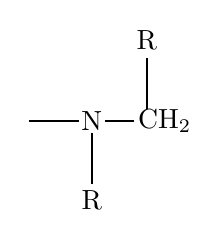
\begin{tikzpicture}[line width=.8pt,>=Stealth,baseline=(current bounding box.center)]
\node[anchor=center,fill=white,inner sep=1pt]at(-0.5,0){$\mathrm{N}$};\draw[](-1.3,0)--(-0.66,0);\node[anchor=west,fill=white,inner sep=1pt]at(0.04,0){$\mathrm{CH_2}$};\draw[](-0.33,0)--(0.04,0);\draw[](-0.5,-0.15)--(-0.5,-0.8);\node[anchor=center,fill=white,inner sep=1pt]at(-0.5,-1){$\mathrm{R}$};\draw[](0.2,0.15)--(0.2,0.8);\node[anchor=center,fill=white,inner sep=1pt]at(0.2,1.03){$\mathrm{R}$};
\end{tikzpicture}}\end{center}
\par 核对入口：\url{https://openstax.org/books/organic-chemistry/pages/24-3-basicity-of-amines}
\par\medskip\clearpage\subsection*{6．（1分）}\textbf{参考答案：B}\par\medskip{}\subsection*{独立推导}
\par 分子内氢键要求同一分子同时有给体、受体，并能以合理距离与方向接近，不能只看到N/O就肯定。
\par B的酚羟基与醛基在苯环间位，刚性骨架不能形成邻羟基苯甲醛的近程稳定O-H...O=C准环。它仍可形成分子间氢键。
\par A的邻位NH/硝基O、C的邻羟基/醛氧及D邻螺原子两侧可接近的OH均可形成分子内氢键。故唯一B。
\subsection*{各选项依据}
\par\textbf{A：}NH与邻位硝基O可形成分子内N-H...O。
\par\textbf{B：}间位OH与CHO不能实现其余各项的近程闭合几何，应选。
\par\textbf{C：}邻羟基苯甲醛可形成六元准环氢键。
\par\textbf{D：}五元环及O-H可转动，邻螺位两个OH可作为给受体接近，不应误按平面图判断。
\subsection*{第三轮反校}
\par B为间位、C为邻位，未交换；A的NO2位于带H的环N附近。
\par D为两五元环共用一个螺原子，环碳共9个，两OH均邻螺位。
\par 能形成不等于在所有介质、温度下该构象均占优势；未编造能量、占比或谱值。
\subsection*{适用边界}
教材分子内氢键定性几何判断，不作定量氢键强度排名。
\begin{center}\resizebox{.35\linewidth}{!}{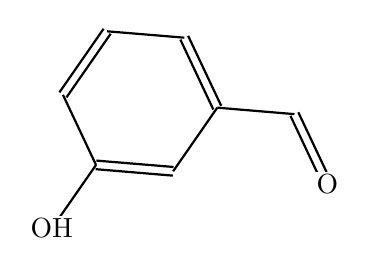
\begin{tikzpicture}[line width=.8pt,baseline=(current bounding box.center)]
\draw (1.800,-0.666)--(1.380,0.223);
\draw (1.700,-0.713)--(1.281,0.177);
\draw (1.331,0.200)--(0.351,0.282);
\draw (0.401,0.305)--(-0.019,1.194);
\draw (0.301,0.258)--(-0.118,1.147);
\draw (-0.068,1.171)--(-1.048,1.252);
\draw (-1.093,1.284)--(-1.654,0.476);
\draw (-1.003,1.221)--(-1.564,0.413);
\draw (-1.609,0.445)--(-1.189,-0.445);
\draw (-1.189,-0.445)--(-1.750,-1.252);
\draw (-1.194,-0.499)--(-0.214,-0.581);
\draw (-1.185,-0.390)--(-0.205,-0.471);
\draw (-0.210,-0.526)--(0.351,0.282);
\node[fill=white,inner sep=1.1pt]at(1.750,-0.689){$\mathrm{O}$};
\node[fill=white,inner sep=1.1pt]at(-1.750,-1.252){$\mathrm{OH}$};
\end{tikzpicture}}\end{center}
\par\medskip\clearpage\subsection*{7．（1分）}\textbf{参考答案：A}\par\medskip{}\subsection*{独立推导}
\par C9H12的苯系烃有4个不饱和度，选项均是芳香骨架；三元羧酸意味着三条可被氧化成羧基的苄位侧链，排除只有两条侧链的D。
\par 再按环上剩余H的位置对称性数一元硝化产物，不按剩余H总数机械计数：A为1,2,4-三甲基，三个剩余位置互不等价，恰有三种；B的三连续Me给两类H，C的间三甲基给一类H。
\subsection*{各选项依据}
\par\textbf{A：}三侧链可氧化，且三个剩余位置无互相交换的分子对称，符合两个条件。
\par\textbf{B：}1,2,3三甲基的两个端部剩余H等价，只给两种位置异构体。
\par\textbf{C：}1,3,5三甲基三个剩余H等价，只有一种。
\par\textbf{D：}只有乙基和甲基两条苄侧链，不能给题设三元酸。
\subsection*{第三轮反校}
\par 从A反画三个候选硝基位置，彼此不能通过保持全部Me位置的对称操作重合。
\par 不是说三个硝基同时引入，也不把乙基的两个侧链碳分别计成两羧基。
\begin{center}\resizebox{.35\linewidth}{!}{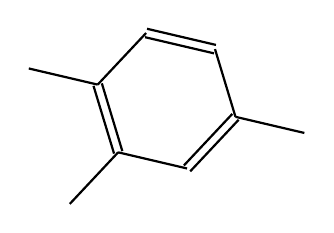
\begin{tikzpicture}[line width=.8pt,>=Stealth,baseline=(current bounding box.center)]
\draw (1.750,-0.184)--(0.875,0.021);
\draw (0.875,0.021)--(0.615,0.881);
\draw (0.627,0.934)--(-0.248,1.139);
\draw (0.602,0.827)--(-0.273,1.032);
\draw (-0.260,1.085)--(-0.875,0.430);
\draw (-0.875,0.430)--(-1.750,0.635);
\draw (-0.928,0.414)--(-0.667,-0.446);
\draw (-0.822,0.446)--(-0.562,-0.414);
\draw (-0.615,-0.430)--(-1.229,-1.085);
\draw (-0.615,-0.430)--(0.260,-0.635);
\draw (0.300,-0.672)--(0.915,-0.017);
\draw (0.220,-0.597)--(0.835,0.058);
\end{tikzpicture}}\end{center}
\par\medskip\clearpage\subsection*{8．（1分）}\textbf{参考答案：A}\par\medskip{}\subsection*{独立推导}
\par 酸处理后标作(a)的物质还要经历臭氧还原裂解，并给两个酮，因此(a)应有一条两端都连两个碳取代基的C=C。中间产物不是凡在机理中出现过的正离子都可以填入。
\par A的双键两端各带一个Me和环骨架碳，裂解分别变成乙酰基。断开该双键后原其余骨架连成五元环，得到原图1,3-二乙酰基环戊烷。酸脱水可经失水、邻位甲基迁移及去H+形成此烯烃，臭氧产物反过来确定迁移后的连接。
\subsection*{各选项依据}
\par\textbf{A：}中性烯烃可逐碳反推出两乙酰基和五元环，符合全部数据。
\par\textbf{B：}质子化醇仍无C=C，不是紧接臭氧裂解的独立中间产物。
\par\textbf{C：}碳正离子不是画出的一条可直接臭氧裂成双酮的烯键；不能只因它可能在脱水机理出现而选。
\par\textbf{D：}同为正离子且Me连接不同，不能回代指定双酮。
\subsection*{第三轮反校}
\par 两Me始终各1C，笼状其余7C；总9C，裂解产物5环C+两乙酰4C仍9。
\par 把A的C=C两端都改为C=O再只展开剩余$\sigma$图，得到五元环1,3-二乙酰，不把交叉桥线当额外结点。
\begin{center}\resizebox{.35\linewidth}{!}{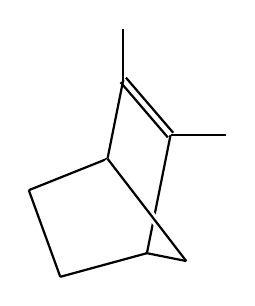
\begin{tikzpicture}[line width=.8pt,>=Stealth,baseline=(current bounding box.center)]
\draw[](0,0)--(-1,-0.4);
\draw[](-1,-0.4)--(-0.6,-1.5);
\draw[](-0.6,-1.5)--(0.5,-1.2);
\draw[](0,0)--(0.2,1);
\draw(0.1658,0.9707)--(0.7658,0.2707);
\draw(0.2342,1.0293)--(0.8342,0.3293);
\draw[](0.8,0.3)--(0.5,-1.2);
\draw[preaction={draw=white,line width=3pt}](0,0)--(1,-1.3);
\draw[](1,-1.3)--(0.5,-1.2);\draw[](0.2,1)--(0.2,1.65);\draw[](0.8,0.3)--(1.5,0.3);
\end{tikzpicture}}\end{center}
\par\medskip\clearpage\subsection*{9．（1分）}\textbf{参考答案：C}\par\medskip{}\subsection*{独立推导}
\par 先核原积分总数：3+6+8+2+1=20H。0.9处3H双峰提示与一个CH相邻的Me；1.1处6H单峰提示连在无邻H碳上的两Me。6.5处1H单峰要求存在一个相对孤立的烯H。
\par C同时具备饱和CH(Me)、一个季碳上的gem-Me2、一个共轭烯酮烯H、以及CO另一侧邻季碳的CH2（可在2.3附近给2H单峰）。其余饱和CH/CH2和Me相邻CH共8H在2.0—2.2多重区，符合原分组。这里按教材简化谱，不把实际所有CH2都宣称永远磁等价。
\subsection*{各选项依据}
\par\textbf{A：}A两条外双键均无烯H，无法给6.5处1H。
\par\textbf{B：}有烯H但两Me在烯碳外端，且另有COCH3；不满足1.1处饱和gem-Me2及2.3处2H的组合。
\par\textbf{C：}五组积分、裂分和局部官能团同时相符。
\par\textbf{D：}外双键同样全取代，缺少6.5处所需烯H。
\subsection*{第三轮反校}
\par 由C逐组回计3H（CHMe）+6H（gem-Me）+2H（COCH2）+1H（烯H）+8H（其他）=20，原$\delta$2.3确为2H而非3H，未改书。
\par 对原图C/D的环上CO和gem-Me/外双键位置重读修正绘图；A/D非同一结构，未偷合并。
\subsection*{适用边界}
本题用原书分组的一级近似。实际稠环CH2可能有非等价、远程耦合和重叠，不能把题给s当普适高分辨定律。
\begin{center}\resizebox{.35\linewidth}{!}{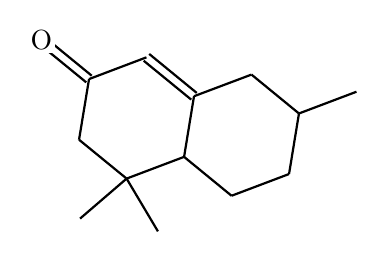
\begin{tikzpicture}[line width=.8pt,>=Stealth,baseline=(current bounding box.center)]
\draw (-2.035,1.172)--(-1.431,0.678);
\draw (-1.965,1.257)--(-1.362,0.763);
\draw (-1.396,0.720)--(-1.523,-0.050);
\draw (-1.523,-0.050)--(-0.919,-0.544);
\draw (-0.919,-0.544)--(-0.521,-1.214);
\draw (-0.919,-0.544)--(-1.510,-1.052);
\draw (-0.919,-0.544)--(-0.189,-0.268);
\draw (-0.189,-0.268)--(0.414,-0.762);
\draw (0.414,-0.762)--(1.144,-0.486);
\draw (1.144,-0.486)--(1.270,0.283);
\draw (1.270,0.283)--(2.000,0.559);
\draw (1.270,0.283)--(0.667,0.777);
\draw (0.667,0.777)--(-0.063,0.502);
\draw (-0.028,0.544)--(-0.632,1.039);
\draw (-0.098,0.459)--(-0.702,0.953);
\draw (-0.667,0.996)--(-1.396,0.720);
\draw (-0.063,0.502)--(-0.189,-0.268);
\node[fill=white,inner sep=1.1pt]at(-2.000,1.214){$\mathrm{O}$};
\end{tikzpicture}}\end{center}\par\medskip\clearpage\subsection*{10．（1分）}\textbf{参考答案：2}\par\medskip{}原书1.6同步练习3；印37页/PDF42页。\par 下列$R^{+}$中最稳定的是：\par\medskip
\begin{minipage}[c][3.4cm][c]{.48\linewidth}\centering (1)\par\smallskip \scalebox{.73}{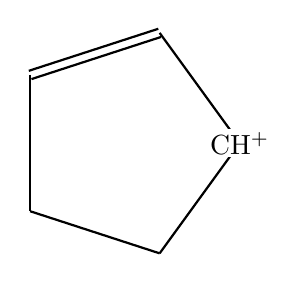
\begin{tikzpicture}[line width=.8pt]\draw (1.331,0.000)--(0.314,1.400);
\draw (0.297,1.452)--(-1.348,0.918);
\draw (0.331,1.348)--(-1.314,0.813);
\draw (-1.331,0.865)--(-1.331,-0.865);
\draw (-1.331,-0.865)--(0.314,-1.400);
\draw (0.314,-1.400)--(1.331,0.000);
\node[fill=white,inner sep=1.1pt]at(1.331,0.000){$\mathrm{CH^{+}}$};\end{tikzpicture}}\end{minipage}\hfill
\begin{minipage}[c][3.4cm][c]{.48\linewidth}\centering (2)\par\smallskip \scalebox{.73}{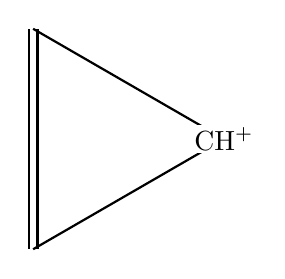
\begin{tikzpicture}[line width=.8pt]\draw (1.212,-0.000)--(-1.212,1.400);
\draw (-1.267,1.400)--(-1.267,-1.400);
\draw (-1.157,1.400)--(-1.157,-1.400);
\draw (-1.212,-1.400)--(1.212,-0.000);
\node[fill=white,inner sep=1.1pt]at(1.212,-0.000){$\mathrm{CH^{+}}$};\end{tikzpicture}}\end{minipage}\par
\begin{minipage}[c][3.4cm][c]{.48\linewidth}\centering (3)\par\smallskip \scalebox{.73}{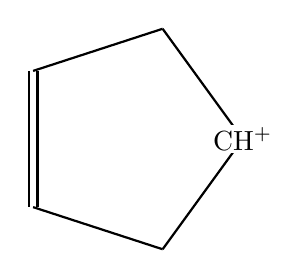
\begin{tikzpicture}[line width=.8pt]\draw (1.331,0.000)--(0.314,1.400);
\draw (0.314,1.400)--(-1.331,0.865);
\draw (-1.386,0.865)--(-1.386,-0.865);
\draw (-1.276,0.865)--(-1.276,-0.865);
\draw (-1.331,-0.865)--(0.314,-1.400);
\draw (0.314,-1.400)--(1.331,0.000);
\node[fill=white,inner sep=1.1pt]at(1.331,0.000){$\mathrm{CH^{+}}$};\end{tikzpicture}}\end{minipage}\hfill
\begin{minipage}[c][3.4cm][c]{.48\linewidth}\centering (4)\par\smallskip \scalebox{.73}{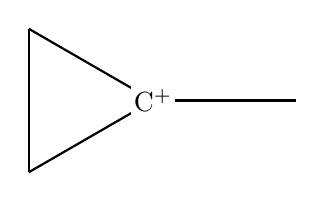
\begin{tikzpicture}[line width=.8pt]\draw (1.700,0.000)--(-0.122,-0.000);
\draw (-0.122,-0.000)--(-1.700,0.911);
\draw (-1.700,0.911)--(-1.700,-0.911);
\draw (-1.700,-0.911)--(-0.122,-0.000);
\node[fill=white,inner sep=1.1pt]at(-0.122,-0.000){$\mathrm{C^{+}}$};\end{tikzpicture}}\end{minipage}\par
\textbf{答案：}(2)。\par\textbf{从基础到判断：}碳正离子稳定性不能只看一级、二级、三级；有芳香稳定化时，应先检查完整环形共轭。环丙烯正离子有三套相邻p轨道、2个\(\pi\)电子，占据最低成键\(\pi\)轨道，满足4n+2（n=0），是本组最佳稳定项(2)。\par\textbf{逐项核验：}\begin{enumerate}
\item 环戊烯基烯丙型正离子可获局部共振稳定，但饱和碳使其不构成完整芳香环，低于(2)。
\item 环丙烯正离子：2\(\pi\)电子芳香体系，选。
\item 双键与正电中心隔有饱和碳，不能当成(1)那样直接的烯丙共轭，也无完整芳香性。
\item 甲基取代环丙基正离子可有超共轭/\(\sigma\)离域，但没有所画环丙烯正离子的闭壳层2\(\pi\)芳香结构，不选。
\end{enumerate}\textbf{易错与边界：}小环张力并不自动排除芳香性；同样，带正电也不自动意味着芳香性。此比较按所画结构的教材模型，不捏造各离子的溶液平衡常数。\par\smallskip 第三轮：复核否定词、原标签、逐项连接/电荷与完整共轭；独立判断后对照原书参考答案（PDF245页）一致。\par\medskip\clearpage\subsection*{11．（1分）}\textbf{参考答案：4}\par\medskip{}原书1.6同步练习5；印37页/PDF42页。\par 下列化合物无芳香性的是：\par\medskip
\begin{minipage}[c][3.4cm][c]{.48\linewidth}\centering (1)\par\smallskip \scalebox{.73}{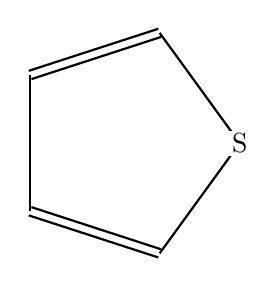
\begin{tikzpicture}[line width=.8pt]\draw (1.331,0.000)--(0.314,1.400);
\draw (0.297,1.452)--(-1.348,0.918);
\draw (0.331,1.348)--(-1.314,0.813);
\draw (-1.331,0.865)--(-1.331,-0.865);
\draw (-1.348,-0.918)--(0.297,-1.452);
\draw (-1.314,-0.813)--(0.331,-1.348);
\draw (0.314,-1.400)--(1.331,0.000);
\node[fill=white,inner sep=1.1pt]at(1.331,0.000){$\mathrm{S}$};\end{tikzpicture}}\end{minipage}\hfill
\begin{minipage}[c][3.4cm][c]{.48\linewidth}\centering (2)\par\smallskip \scalebox{.73}{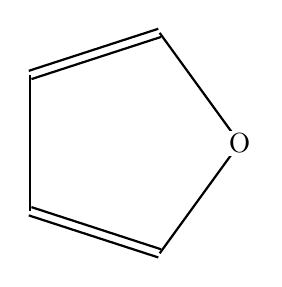
\begin{tikzpicture}[line width=.8pt]\draw (1.331,0.000)--(0.314,1.400);
\draw (0.297,1.452)--(-1.348,0.918);
\draw (0.331,1.348)--(-1.314,0.813);
\draw (-1.331,0.865)--(-1.331,-0.865);
\draw (-1.348,-0.918)--(0.297,-1.452);
\draw (-1.314,-0.813)--(0.331,-1.348);
\draw (0.314,-1.400)--(1.331,0.000);
\node[fill=white,inner sep=1.1pt]at(1.331,0.000){$\mathrm{O}$};\end{tikzpicture}}\end{minipage}\par
\begin{minipage}[c][3.4cm][c]{.48\linewidth}\centering (3)\par\smallskip \scalebox{.73}{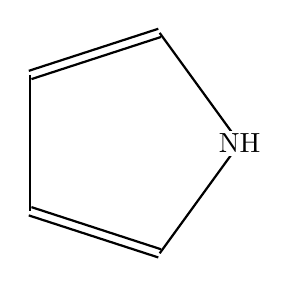
\begin{tikzpicture}[line width=.8pt]\draw (1.331,0.000)--(0.314,1.400);
\draw (0.297,1.452)--(-1.348,0.918);
\draw (0.331,1.348)--(-1.314,0.813);
\draw (-1.331,0.865)--(-1.331,-0.865);
\draw (-1.348,-0.918)--(0.297,-1.452);
\draw (-1.314,-0.813)--(0.331,-1.348);
\draw (0.314,-1.400)--(1.331,0.000);
\node[fill=white,inner sep=1.1pt]at(1.331,0.000){$\mathrm{NH}$};\end{tikzpicture}}\end{minipage}\hfill
\begin{minipage}[c][3.4cm][c]{.48\linewidth}\centering (4)\par\smallskip \scalebox{.73}{\begin{tikzpicture}[line width=.8pt]\draw (1.617,0.000)--(0.808,1.400);
\draw (0.808,1.455)--(-0.808,1.455);
\draw (0.808,1.345)--(-0.808,1.345);
\draw (-0.808,1.400)--(-1.617,0.000);
\draw (-1.617,0.000)--(-0.808,-1.400);
\draw (-0.808,-1.455)--(0.808,-1.455);
\draw (-0.808,-1.345)--(0.808,-1.345);
\draw (0.808,-1.400)--(1.617,0.000);
\node[fill=white,inner sep=1.1pt]at(1.617,0.000){$\mathrm{O}$};\end{tikzpicture}}\end{minipage}\par
\textbf{答案：}(4)。\par\textbf{从基础到判断：}检查杂环芳香性时，先找环内是否有sp3碳阻断共轭；没有阻断才数\(\pi\)电子。噻吩、呋喃和吡咯都具有两条双键及一对参与共轭的杂原子孤电子，共6\(\pi\)电子；第四项吡喃含一个饱和CH2，环形共轭中断，所以无芳香性者为(4)。\par\textbf{逐项核验：}\begin{enumerate}
\item 噻吩：两条C=C供4电子，S一对孤电子供2，6\(\pi\)芳香，不选。
\item 呋喃：O只用一对孤电子参与\(\pi\)系统，合计6\(\pi\)，不选。
\item 吡咯：N孤电子参与形成6\(\pi\)体系；N—H不妨碍芳香性，不选。
\item 4H-吡喃：环上CH2是sp3碳，虽有O与两条双键，不能沿整个环连续共轭，选。
\end{enumerate}\textbf{易错与边界：}不能把氧的两对孤电子都加进同一个\(\pi\)环，也不能见“两条双键加一对孤电子”就跳过连续共轭检查。\par\smallskip 第三轮：复核否定词、原标签、逐项连接/电荷与完整共轭；独立判断后对照原书参考答案（PDF245页）一致。\par\medskip\clearpage\subsection*{12．（1分）}\textbf{参考答案：1}\par\medskip{}原书1.6同步练习7；印37页/PDF42页。\par 下列碳正离子中最稳定的是：\par\medskip
\begin{minipage}[c][3.4cm][c]{.48\linewidth}\centering (1)\par\smallskip \scalebox{.73}{\begin{tikzpicture}[line width=.8pt]\draw (1.365,-0.000)--(0.824,1.123);
\draw (0.836,1.176)--(-0.378,1.454);
\draw (0.812,1.069)--(-0.403,1.346);
\draw (-0.391,1.400)--(-1.365,0.623);
\draw (-1.420,0.623)--(-1.420,-0.623);
\draw (-1.310,0.623)--(-1.310,-0.623);
\draw (-1.365,-0.623)--(-0.391,-1.400);
\draw (-0.378,-1.454)--(0.836,-1.176);
\draw (-0.403,-1.346)--(0.812,-1.069);
\draw (0.824,-1.123)--(1.365,-0.000);
\node[fill=white,inner sep=1.1pt]at(1.365,-0.000){$\mathrm{CH^{+}}$};\end{tikzpicture}}\end{minipage}\hfill
\begin{minipage}[c][3.4cm][c]{.48\linewidth}\centering (2)\par\smallskip \scalebox{.73}{\begin{tikzpicture}[line width=.8pt]\draw (1.617,0.000)--(0.808,1.400);
\draw (0.808,1.455)--(-0.808,1.455);
\draw (0.808,1.345)--(-0.808,1.345);
\draw (-0.808,1.400)--(-1.617,0.000);
\draw (-1.617,0.000)--(-0.808,-1.400);
\draw (-0.808,-1.455)--(0.808,-1.455);
\draw (-0.808,-1.345)--(0.808,-1.345);
\draw (0.808,-1.400)--(1.617,0.000);
\node[fill=white,inner sep=1.1pt]at(1.617,0.000){$\mathrm{CH^{+}}$};\end{tikzpicture}}\end{minipage}\par
\begin{minipage}[c][3.4cm][c]{.48\linewidth}\centering (3)\par\smallskip \scalebox{.73}{\begin{tikzpicture}[line width=.8pt]\draw (1.617,0.000)--(0.808,1.400);
\draw (0.808,1.400)--(-0.808,1.400);
\draw (-0.808,1.400)--(-1.617,0.000);
\draw (-1.617,0.000)--(-0.808,-1.400);
\draw (-0.808,-1.400)--(0.808,-1.400);
\draw (0.808,-1.400)--(1.617,0.000);
\node[fill=white,inner sep=1.1pt]at(1.617,0.000){$\mathrm{CH^{+}}$};\end{tikzpicture}}\end{minipage}\hfill
\begin{minipage}[c][3.4cm][c]{.48\linewidth}\centering (4)\par\smallskip \scalebox{.73}{\begin{tikzpicture}[line width=.8pt]\draw (1.400,-0.000)--(0.000,1.400);
\draw (0.000,1.400)--(-1.400,0.000);
\draw (-1.400,0.000)--(-0.000,-1.400);
\draw (-0.000,-1.400)--(1.400,-0.000);
\node[fill=white,inner sep=1.1pt]at(1.400,-0.000){$\mathrm{CH^{+}}$};\end{tikzpicture}}\end{minipage}\par
\textbf{答案：}(1)。\par\textbf{从基础到判断：}先找共轭范围，再比较稳定化机制。环庚三烯正离子有7个连续p轨道、6\(\pi\)电子，正电荷可在整个环离域，满足Hückel闭壳层规则，因此本组最稳定的是(1)。\par\textbf{逐项核验：}\begin{enumerate}
\item 环庚三烯正离子：完整6\(\pi\)芳香环，选。
\item 环己二烯基正离子仍含饱和碳，最多为局部共轭正离子，不是完整芳香环。
\item 环己基正离子没有相邻\(\pi\)系统提供芳香离域，不选。
\item 环丁基正离子也没有所画(1)的6\(\pi\)闭壳层环形共轭，不能因环小而优先，不选。
\end{enumerate}\textbf{易错与边界：}“有共振”不等于“芳香”。不要把(2)补画成苯环，补一条双键会改变原题结构和形式价态。\par\smallskip 第三轮：复核否定词、原标签、逐项连接/电荷与完整共轭；独立判断后对照原书参考答案（PDF245页）一致。\par\medskip\clearpage\clearpage\section*{三、结构推导（5题，共35分）}\subsection*{1．（4分）}一个无色的固体$\mathrm{C_{10}H_{13}NO}$，它的核磁共振氢谱如下，试推测它的结构。
\begin{center}\resizebox{.87\linewidth}{!}{\begin{tikzpicture}[line width=.8pt,>=Stealth,baseline=(current bounding box.center)]
\draw(0,0)--(12,0);
\draw(12.0,0)--(12.0,-.12)node[below]{$0$};
\draw(10.666666666666666,0)--(10.666666666666666,-.12)node[below]{$1$};
\draw(9.333333333333334,0)--(9.333333333333334,-.12)node[below]{$2$};
\draw(8.0,0)--(8.0,-.12)node[below]{$3$};
\draw(6.666666666666667,0)--(6.666666666666667,-.12)node[below]{$4$};
\draw(5.333333333333333,0)--(5.333333333333333,-.12)node[below]{$5$};
\draw(4.0,0)--(4.0,-.12)node[below]{$6$};
\draw(2.6666666666666665,0)--(2.6666666666666665,-.12)node[below]{$7$};
\draw(1.3333333333333333,0)--(1.3333333333333333,-.12)node[below]{$8$};
\draw(0.0,0)--(0.0,-.12)node[below]{$9$};
\node at(6,-1.5){$\delta$};
\draw[blue!60!black,line width=.5pt](2.3600000000000003,0)--(2.3600000000000003,0.7999999999999999);
\draw[blue!60!black,line width=.5pt](2.3133333333333335,0)--(2.3133333333333335,1.5999999999999999);
\draw[blue!60!black,line width=.5pt](2.266666666666667,0)--(2.266666666666667,2.4);
\draw[blue!60!black,line width=.5pt](2.2200000000000006,0)--(2.2200000000000006,1.5999999999999999);
\draw[blue!60!black,line width=.5pt](2.173333333333334,0)--(2.173333333333334,0.7999999999999999);
\draw[red!50!black](2.016666666666667,0.2)--(2.206666666666667,0.2)--(2.316666666666667,0.7)--(2.566666666666667,0.7);
\draw[blue!60!black,line width=.5pt](3.7866666666666666,0)--(3.7866666666666666,0.048);
\draw[blue!60!black,line width=.5pt](3.626666666666667,0)--(3.626666666666667,0.096);
\draw[blue!60!black,line width=.5pt](3.4666666666666663,0)--(3.4666666666666663,0.12);
\draw[blue!60!black,line width=.5pt](3.306666666666666,0)--(3.306666666666666,0.096);
\draw[blue!60!black,line width=.5pt](3.146666666666666,0)--(3.146666666666666,0.048);
\draw[red!50!black](3.2166666666666663,0.7)--(3.4066666666666663,0.7)--(3.516666666666666,0.8)--(3.766666666666666,0.8);
\draw[blue!60!black,line width=.5pt](7.453333333333333,0)--(7.453333333333333,0.3);
\draw[blue!60!black,line width=.5pt](7.333333333333333,0)--(7.333333333333333,0.6);
\draw[blue!60!black,line width=.5pt](7.213333333333334,0)--(7.213333333333334,0.3);
\draw[red!50!black](7.083333333333333,0.8)--(7.273333333333333,0.8)--(7.383333333333333,1.0)--(7.633333333333333,1.0);
\draw[blue!60!black,line width=.5pt](8.266666666666666,0)--(8.266666666666666,0.35);
\draw[blue!60!black,line width=.5pt](8.133333333333333,0)--(8.133333333333333,0.7);
\draw[blue!60!black,line width=.5pt](8.0,0)--(8.0,0.35);
\draw[red!50!black](7.883333333333333,1.0)--(8.073333333333332,1.0)--(8.183333333333334,1.2)--(8.433333333333334,1.2);
\draw[blue!60!black,line width=.5pt](9.333333333333334,0)--(9.333333333333334,2.3);
\draw[red!50!black](9.083333333333334,1.2)--(9.273333333333333,1.2)--(9.383333333333335,1.5)--(9.633333333333335,1.5);
\draw[blue!60!black,line width=.45pt](11.92,0)--(11.95,0)--(11.97,0.1)--(11.99,0)--(12.02,0);
\end{tikzpicture}}\end{center}
\subsection*{答案与边界}
N-(2-苯乙基)乙酰胺$\mathrm{PhCH_2CH_2NHCOCH_3}$。
\begin{center}\resizebox{.50\linewidth}{!}{\begin{tikzpicture}[line width=.8pt,>=Stealth,baseline=(current bounding box.center)]
\draw (-2.000,-0.249)--(-1.407,0.005);
\draw (-1.352,-0.001)--(-1.276,0.640);
\draw (-1.461,0.012)--(-1.385,0.653);
\draw (-1.407,0.005)--(-0.890,-0.381);
\draw (-0.890,-0.381)--(-0.297,-0.127);
\draw (-0.297,-0.127)--(0.220,-0.514);
\draw (0.220,-0.514)--(0.813,-0.259);
\draw (0.781,-0.304)--(1.297,-0.690);
\draw (0.846,-0.215)--(1.363,-0.602);
\draw (1.330,-0.646)--(1.924,-0.392);
\draw (1.978,-0.398)--(2.055,0.243);
\draw (1.869,-0.385)--(1.945,0.256);
\draw (2.000,0.249)--(1.483,0.636);
\draw (1.461,0.686)--(0.868,0.432);
\draw (1.505,0.585)--(0.912,0.331);
\draw (0.890,0.381)--(0.813,-0.259);
\node[fill=white,inner sep=1.1pt]at(-1.330,0.646){$\mathrm{O}$};
\node[fill=white,inner sep=1.1pt]at(-0.890,-0.381){$\mathrm{NH}$};
\node at(0.0,-1.7){$\mathrm{}$};
\end{tikzpicture}}\end{center}
\subsection*{独立推导}
\par 含N的DBE=5，可由苯环4+羰基1组成。芳香5H支持单取代苯。
\par 约2处3H单峰为乙酰Me；约3与3.5的两组2H为苄CH2及邻N的CH2；余1H宽信号为NH。拼接为PhCH2CH2NHCOCH3。
\par NH峰形/位置受介质、温度、交换影响，不能据手绘曲线额外生成精确ppm或J值。
\subsection*{第三轮化学反校}
\par Ph6C+2CH2+乙酰2C=10C；5+2+2+1+3=13H，N/O各1。
\par 若为PhCONHCH2CH2CH3，必须有末端Me三重峰而不是乙酰3H单峰，且脂肪分组不同。
\subsection*{参考采分点（编辑建议）}
\par 下列为编辑建议，非原书官方评分。
\par 4分：DBE1；谱段1；连接1；氢数核对1。
\par\vspace{3mm}\footnotesize 来源：S01；PDF 82；印刷 76；题号5-78。\normalsize
\par\medskip\clearpage\subsection*{2．（10分）}(A)分子式$\mathrm{C_7H_{12}}$，在$\mathrm{KMnO_4-H_2O}$中加热回流，反应液中只有环己酮。(A)与HCl得(B)，(B)在$\mathrm{C_2H_5ONa-C_2H_5OH}$中得(C)。(C)使$\mathrm{Br_2}$褪色生成(D)，(D)用同样乙醇钠/乙醇处理生成(E)；(E)经热高锰酸钾得$\mathrm{HOOCCH_2CH_2COOH}$和$\mathrm{CH_3COCOOH}$；(C)经$\mathrm{O_3}$再用$\mathrm{Zn,H_2O}$得$\mathrm{CH_3COCH_2CH_2CH_2CH_2CHO}$。写出(A)构造式，并用反应式说明结构正确。

\subsection*{答案与边界}
A亚甲基环己烷；B 1-氯-1-甲基环己烷；C 1-甲基环己烯；D 反式1,2-二溴-1-甲基环己烷（外消旋）；E 1-甲基环己-1,3-二烯。
\begin{center}\resizebox{.50\linewidth}{!}{\begin{tikzpicture}[line width=.8pt,>=Stealth,baseline=(current bounding box.center)]
\draw (2.000,0.055)--(0.667,0.055);
\draw (2.000,-0.055)--(0.667,-0.055);
\draw (0.667,0.000)--(0.000,1.155);
\draw (0.000,1.155)--(-1.333,1.155);
\draw (-1.333,1.155)--(-2.000,0.000);
\draw (-2.000,0.000)--(-1.333,-1.155);
\draw (-1.333,-1.155)--(-0.000,-1.155);
\draw (-0.000,-1.155)--(0.667,0.000);
\node at(0.0,-1.7){$\mathrm{A}$};
\draw (7.800,0.930)--(6.692,0.000);
\draw (6.692,0.000)--(7.800,-0.930);
\draw (6.692,0.000)--(5.969,1.252);
\draw (5.969,1.252)--(4.523,1.252);
\draw (4.523,1.252)--(3.800,0.000);
\draw (3.800,0.000)--(4.523,-1.252);
\draw (4.523,-1.252)--(5.969,-1.252);
\draw (5.969,-1.252)--(6.692,0.000);
\node[fill=white,inner sep=1.1pt]at(7.800,-0.930){$\mathrm{Cl}$};
\node at(5.8,-1.7){$\mathrm{B}$};
\draw (2.000,-3.800)--(0.667,-3.800);
\draw (0.714,-3.772)--(0.048,-2.618);
\draw (0.619,-3.827)--(-0.048,-2.673);
\draw (0.000,-2.645)--(-1.333,-2.645);
\draw (-1.333,-2.645)--(-2.000,-3.800);
\draw (-2.000,-3.800)--(-1.333,-4.955);
\draw (-1.333,-4.955)--(-0.000,-4.955);
\draw (-0.000,-4.955)--(0.667,-3.800);
\node at(0.0,-5.5){$\mathrm{C}$};
\draw (7.800,-3.800)--(6.467,-3.800);
\draw (6.514,-3.772)--(5.848,-2.618);
\draw (6.419,-3.827)--(5.752,-2.673);
\draw (5.800,-2.645)--(4.467,-2.645);
\draw (4.419,-2.618)--(3.752,-3.772);
\draw (4.514,-2.673)--(3.848,-3.827);
\draw (3.800,-3.800)--(4.467,-4.955);
\draw (4.467,-4.955)--(5.800,-4.955);
\draw (5.800,-4.955)--(6.467,-3.800);
\node at(5.8,-5.5){$\mathrm{E}$};
\end{tikzpicture}}\end{center}\par D：\begin{center}\resizebox{.50\linewidth}{!}{\begin{tikzpicture}[line width=.8pt,>=Stealth,baseline=(current bounding box.center)]
\draw[](1,0)--(0.5,-0.87);\draw[](0.5,-0.87)--(-0.5,-0.87);\draw[](-0.5,-0.87)--(-1,0);\draw[](-1,0)--(-0.5,0.87);\draw[](-0.5,0.87)--(0.5,0.87);\draw[](0.5,0.87)--(1,0);\fill(1,0)--(1.768695048315003,0.46260990336999414)--(1.831304951684997,0.3373900966300059)--cycle;\node[fill=white,inner sep=1pt]at(2,0.55){$\mathrm{Br}$};\draw[densely dashed](1,0)--(1.8,-0.4);\node[fill=white,inner sep=1pt]at(2,-0.55){$\mathrm{CH_3}$};\draw[densely dashed](0.5,-0.87)--(0.9,-1.7);\node[fill=white,inner sep=1pt]at(1,-1.95){$\mathrm{Br}$};\fill(0.5,-0.87)--(-0.04751135012444352,-1.5963135145960794)--(-0.1524886498755565,-1.5036864854039207)--cycle;\node[fill=white,inner sep=1pt]at(-0.2,-1.8){$\mathrm{H}$};\node at(0,-2.5){$(\pm)$};
\end{tikzpicture}}\end{center}
\subsection*{独立推导}
\par 热氧化裂解给环己酮说明被裂解烯碳在环上，另端为=CH2；末端碳可最终成为CO2，不能把其“消失”理解为不守恒。
\par 马氏加HCl得叔卤B；消去较多取代烯C。C还原臭氧断环给一端甲基酮、一端醛，中间四CH2，符合题给七碳羰基物。
\par Br2经桥式溴带正电离子中间体反加成给两Br反式D；合适双直立/反式共平面构象失两HBr得到共轭E。E氧化切两双键给丁二酸与丙酮酸。
\subsection*{第三轮化学反校}
\par 碳账A氧化6+1，C臭氧7，E氧化4+3，均为7C。
\par D为C7H12Br2，失2HBr成为C7H10；D相对Br反式，绝对构型未指定故以一对对映体表示。
\par 热KMnO4将带H烯C氧化为COOH，而Zn还原臭氧保留CHO；两类氧化条件不可混写。
\subsection*{参考采分点（编辑建议）}
\par 下列为编辑建议，非原书官方评分。
\par 10分：A2；B1；C1；D反式与外消旋2；E2；裂解计量2。
\par\vspace{3mm}\footnotesize 来源：S01；PDF 156,157；印刷 150,151；题号8-67。\normalsize
\par\medskip\clearpage\subsection*{3．（10分）}A分子式$\mathrm{C_5H_{10}O_2}$，与二当量溴化乙烯基镁反应得B/C混合物，不能简单蒸馏分开。用乙酸—乙酐和催化量对甲苯磺酸在$0\,^{\circ}\mathrm C$处理，蒸馏得较低沸点未反应C和高沸点D/E混合物，后者仍不能简单蒸馏分开。D/E与原图所示醌反应生成结晶F，母液回收未反应E，约为D/E混合物一半。E为D的立体异构体，式$\mathrm{C_9H_{14}O_2}$，结构如下。C为$\mathrm{C_7H_{12}O}$；IR：1725、1645、920 $\mathrm{cm^{-1}}$；氢谱：1.10(3H,t)、2.38(6H,m)、4.94(1H,d,$J=11$ Hz)、5.10(1H,d,$J=17$ Hz)、5.4—6.2(1H,m)。推断A—D、F结构，并归属C光谱。\par\textit{编辑注：醌试剂据原书明确结构式绘为对苯醌；原书正文误称“萘醌”，该文字冲突另档保留。}
\textbf{E}\begin{center}\resizebox{.50\linewidth}{!}{\begin{tikzpicture}[line width=.8pt,>=Stealth,baseline=(current bounding box.center)]
\draw (1.489,0.705)--(0.895,0.424);
\draw (1.536,0.606)--(0.942,0.324);
\draw (0.918,0.374)--(0.865,-0.281);
\draw (0.865,-0.281)--(1.406,-0.655);
\draw (1.406,-0.655)--(2.000,-0.374);
\draw (0.841,-0.232)--(0.247,-0.513);
\draw (0.888,-0.331)--(0.294,-0.612);
\draw (0.270,-0.563)--(-0.270,-0.189);
\draw (-0.270,-0.189)--(-0.865,-0.470);
\draw (-0.865,-0.470)--(-1.406,-0.096);
\draw (-1.406,-0.096)--(-2.000,-0.377);
\draw (-1.351,-0.101)--(-1.297,0.555);
\draw (-1.460,-0.092)--(-1.407,0.564);
\node[fill=white,inner sep=1.1pt]at(-0.865,-0.470){$\mathrm{O}$};
\node[fill=white,inner sep=1.1pt]at(-1.352,0.559){$\mathrm{O}$};
\node at(0.0,-1.7){$\mathrm{}$};
\end{tikzpicture}}\end{center}\par\textbf{原流程所画醌}\begin{center}\resizebox{.50\linewidth}{!}{\begin{tikzpicture}[line width=.8pt,>=Stealth,baseline=(current bounding box.center)]
\draw (2.000,0.055)--(1.000,0.055);
\draw (2.000,-0.055)--(1.000,-0.055);
\draw (1.000,0.000)--(0.500,0.866);
\draw (0.500,0.921)--(-0.500,0.921);
\draw (0.500,0.811)--(-0.500,0.811);
\draw (-0.500,0.866)--(-1.000,0.000);
\draw (-1.000,0.055)--(-2.000,0.055);
\draw (-1.000,-0.055)--(-2.000,-0.055);
\draw (-1.000,0.000)--(-0.500,-0.866);
\draw (-0.500,-0.921)--(0.500,-0.921);
\draw (-0.500,-0.811)--(0.500,-0.811);
\draw (0.500,-0.866)--(1.000,0.000);
\node[fill=white,inner sep=1.1pt]at(2.000,0.000){$\mathrm{O}$};
\node[fill=white,inner sep=1.1pt]at(-2.000,0.000){$\mathrm{O}$};
\node at(0.0,-1.7){$\mathrm{}$};
\end{tikzpicture}}\end{center}
\subsection*{答案与边界}
A丙酸乙酯；B 3-乙基戊-1,4-二烯-3-醇；C庚-6-烯-3-酮；D (2E)-3-乙基戊-2,4-二烯-1-基乙酸酯，E为对应2Z体；F连接结构为D与原图对苯醌的Diels—Alder加成物。题设不足以唯一给出F绝对构型，连接图不冒称完整立体证据。
\begin{center}\resizebox{.50\linewidth}{!}{\begin{tikzpicture}[line width=.8pt,>=Stealth,baseline=(current bounding box.center)]
\draw (-2.000,0.342)--(-1.165,0.723);
\draw (-1.165,0.723)--(-0.417,0.191);
\draw (-0.472,0.196)--(-0.559,-0.718);
\draw (-0.363,0.185)--(-0.450,-0.728);
\draw (-0.417,0.191)--(0.417,0.572);
\draw (0.417,0.572)--(1.165,0.040);
\draw (1.165,0.040)--(2.000,0.421);
\node[fill=white,inner sep=1.1pt]at(-0.505,-0.723){$\mathrm{O}$};
\node[fill=white,inner sep=1.1pt]at(0.417,0.572){$\mathrm{O}$};
\node at(0.0,-1.7){$\mathrm{A}$};
\draw (7.542,1.412)--(7.270,0.186);
\draw (7.649,1.388)--(7.378,0.163);
\draw (7.324,0.175)--(6.127,-0.203);
\draw (6.127,-0.203)--(6.504,-1.400);
\draw (6.127,-0.203)--(4.930,-0.580);
\draw (4.930,-0.580)--(4.004,0.268);
\draw (6.127,-0.203)--(5.749,0.994);
\draw (5.761,1.048)--(4.536,1.320);
\draw (5.738,0.941)--(4.512,1.212);
\node[fill=white,inner sep=1.1pt]at(6.504,-1.400){$\mathrm{OH}$};
\node at(5.8,-1.7){$\mathrm{B}$};
\draw (-2.000,-3.561)--(-1.316,-3.207);
\draw (-1.316,-3.207)--(-0.667,-3.623);
\draw (-0.722,-3.620)--(-0.757,-4.390);
\draw (-0.612,-3.625)--(-0.647,-4.395);
\draw (-0.667,-3.623)--(0.018,-3.269);
\draw (0.018,-3.269)--(0.667,-3.684);
\draw (0.667,-3.684)--(1.351,-3.330);
\draw (1.321,-3.376)--(1.970,-3.792);
\draw (1.381,-3.284)--(2.030,-3.699);
\node[fill=white,inner sep=1.1pt]at(-0.702,-4.393){$\mathrm{O}$};
\node at(0.0,-5.5){$\mathrm{C}$};
\draw (3.776,-4.224)--(4.371,-4.505);
\draw (3.824,-4.124)--(4.418,-4.406);
\draw (4.394,-4.455)--(4.935,-4.081);
\draw (4.935,-4.081)--(4.882,-3.426);
\draw (4.882,-3.426)--(4.287,-3.145);
\draw (4.912,-4.131)--(5.506,-4.412);
\draw (4.959,-4.032)--(5.553,-4.313);
\draw (5.530,-4.363)--(6.070,-3.989);
\draw (6.070,-3.989)--(6.665,-4.270);
\draw (6.665,-4.270)--(7.206,-3.896);
\draw (7.206,-3.896)--(7.800,-4.177);
\draw (7.260,-3.892)--(7.207,-3.236);
\draw (7.151,-3.901)--(7.097,-3.245);
\node[fill=white,inner sep=1.1pt]at(6.665,-4.270){$\mathrm{O}$};
\node[fill=white,inner sep=1.1pt]at(7.152,-3.241){$\mathrm{O}$};
\node at(5.8,-5.5){$\mathrm{D-(2E)}$};
\draw (0.169,-8.914)--(0.635,-8.566);
\draw (0.103,-8.825)--(0.569,-8.478);
\draw (0.602,-8.522)--(1.136,-8.752);
\draw (1.169,-8.796)--(1.635,-8.448);
\draw (1.103,-8.707)--(1.569,-8.360);
\draw (1.602,-8.404)--(1.534,-7.826);
\draw (1.567,-7.871)--(2.033,-7.523);
\draw (1.501,-7.782)--(1.967,-7.435);
\draw (1.534,-7.826)--(1.000,-7.597);
\draw (1.000,-7.597)--(0.534,-7.944);
\draw (0.534,-7.944)--(-0.000,-7.715);
\draw (-0.000,-7.715)--(-0.466,-8.063);
\draw (-0.466,-8.063)--(-1.000,-7.833);
\draw (-1.000,-7.833)--(-1.466,-8.181);
\draw (-1.466,-8.181)--(-2.000,-7.951);
\draw (-1.521,-8.187)--(-1.452,-8.764);
\draw (-1.411,-8.174)--(-1.343,-8.751);
\draw (-0.000,-7.715)--(-0.068,-7.137);
\draw (-0.068,-7.137)--(-0.602,-6.908);
\draw (-0.602,-6.908)--(-0.670,-6.330);
\draw (-0.035,-7.182)--(0.431,-6.834);
\draw (-0.101,-7.093)--(0.365,-6.746);
\draw (0.398,-6.790)--(0.932,-7.019);
\draw (0.534,-7.944)--(0.602,-8.522);
\draw (0.932,-7.019)--(1.000,-7.597);
\node[fill=white,inner sep=1.1pt]at(0.136,-8.870){$\mathrm{O}$};
\node[fill=white,inner sep=1.1pt]at(2.000,-7.479){$\mathrm{O}$};
\node[fill=white,inner sep=1.1pt]at(-1.000,-7.833){$\mathrm{O}$};
\node[fill=white,inner sep=1.1pt]at(-1.398,-8.758){$\mathrm{O}$};
\node at(0.0,-9.299999999999999){$\mathrm{F-connectivity}$};
\end{tikzpicture}}\end{center}
\subsection*{独立推导}
\par C的1725为酮C=O，1645及920支持末端CH=CH2。末端CH2两H分别与CH顺/反耦合给11/17 Hz，CH为5.4—6.2；1.10的3H三重峰为乙基Me，其邻羰CH2与另两CH2共6H集中2.38。故C=EtCOCH2CH2CH=CH2。
\par 酯A先经乙烯基Mg进攻与乙氧基离去，形成中间烯酮$\mathrm{EtCOCH=CH_2}$；第二当量乙烯基Mg有两条竞争路径：1,2加成到羰基，水解给$\mathrm{EtC(OH)(CH=CH_2)_2}$即B；1,4加成到烯酮末端，烯醇盐水解给$\mathrm{EtCOCH_2CH_2CH=CH_2}$即C。B/C由竞争加成产生，不能把B说成经氧杂Cope转成C；B只有五碳二烯链，不满足六原子Cope骨架。
\par B经乙酰化/烯丙位转位给3-乙基共轭二烯醇乙酸酯D/E。原E是2Z（优先级vinyl高于Et，CH2OAc高于H，两高优先基同侧）；D为2E。
\par D采用可用s-cis构象进行DA；保留中间C=C、在对苯醌的一条C=C上成两条新单键，得到F的融合双环连接。不能把母液回收约一半误写成普遍50\%定量选择性定律。
\subsection*{第三轮化学反校}
\par C积分3+6+1+1+1=12；A5+两vinyl4−OEt2=7；酰化再加Ac2使D/E9C。
\par 原文字写“萘醌”，但原流程清楚画对苯醌C6H4O2，二者不相同。正式编排必须明确采用图示试剂并记录书中文字错误，不能悄悄冒充完全无改动原文。
\par F=D9C+醌6C=15C；两新sigma键及一条残余新环烯键吻合DA。F端/面选择若需唯一，应另给立体证据；当前只报可由原题确定的连接及D/E几何。
\par 本轮已纠正初稿错误的氧杂Cope表述；按酯→烯酮→1,2/1,4两路逐键回代，产物连接和分子式全部对应。
\subsection*{参考采分点（编辑建议）}
\par 下列为编辑建议，非原书官方评分。
\par 10分：C及归属2；B竞争加成2；A1；D/E几何2；F连接2；守恒1；不要求未给绝对构型。
\par\vspace{3mm}\footnotesize 来源：S03；PDF 202；印刷 197；题号整题。\normalsize
\par\medskip\clearpage\subsection*{4．（5分）}一个硝基化合物，其分子式为$\mathrm{C_3H_6ClNO_2}$，推测它的结构。试解释$\delta=2.3$处多重峰的产生。
\begin{center}\resizebox{.87\linewidth}{!}{\begin{tikzpicture}[line width=.8pt,>=Stealth,baseline=(current bounding box.center)]
\draw(0,0)--(12,0);
\draw(12.0,0)--(12.0,-.12)node[below]{$0$};
\draw(10.666666666666666,0)--(10.666666666666666,-.12)node[below]{$1$};
\draw(9.333333333333334,0)--(9.333333333333334,-.12)node[below]{$2$};
\draw(8.0,0)--(8.0,-.12)node[below]{$3$};
\draw(6.666666666666667,0)--(6.666666666666667,-.12)node[below]{$4$};
\draw(5.333333333333333,0)--(5.333333333333333,-.12)node[below]{$5$};
\draw(4.0,0)--(4.0,-.12)node[below]{$6$};
\draw(2.6666666666666665,0)--(2.6666666666666665,-.12)node[below]{$7$};
\draw(1.3333333333333333,0)--(1.3333333333333333,-.12)node[below]{$8$};
\draw(0.0,0)--(0.0,-.12)node[below]{$9$};
\node at(6,-1.5){$\delta$};
\draw[blue!60!black,line width=.5pt](4.1933333333333325,0)--(4.1933333333333325,1.2);
\draw[blue!60!black,line width=.5pt](4.073333333333333,0)--(4.073333333333333,1.2);
\draw[red!50!black](3.883333333333333,0.2)--(4.073333333333333,0.2)--(4.183333333333333,0.30000000000000004)--(4.433333333333333,0.30000000000000004);
\draw[blue!60!black,line width=.5pt](9.213333333333333,0)--(9.213333333333333,0.175);
\draw[blue!60!black,line width=.5pt](9.12,0)--(9.12,0.35);
\draw[blue!60!black,line width=.5pt](9.026666666666667,0)--(9.026666666666667,0.5249999999999999);
\draw[blue!60!black,line width=.5pt](8.933333333333334,0)--(8.933333333333334,0.7);
\draw[blue!60!black,line width=.5pt](8.84,0)--(8.84,0.5249999999999999);
\draw[blue!60!black,line width=.5pt](8.746666666666666,0)--(8.746666666666666,0.35);
\draw[blue!60!black,line width=.5pt](8.653333333333332,0)--(8.653333333333332,0.175);
\draw[red!50!black](8.683333333333334,0.30000000000000004)--(8.873333333333333,0.30000000000000004)--(8.983333333333334,0.5)--(9.233333333333334,0.5);
\draw[blue!60!black,line width=.5pt](10.399999999999999,0)--(10.399999999999999,1.0);
\draw[blue!60!black,line width=.5pt](10.266666666666667,0)--(10.266666666666667,2.0);
\draw[blue!60!black,line width=.5pt](10.133333333333333,0)--(10.133333333333333,1.0);
\draw[red!50!black](10.016666666666667,0.5)--(10.206666666666667,0.5)--(10.316666666666668,0.8)--(10.566666666666668,0.8);
\draw[blue!60!black,line width=.45pt](11.92,0)--(11.95,0)--(11.97,0.25)--(11.99,0)--(12.02,0);
\end{tikzpicture}}\end{center}
\subsection*{答案与边界}
1-氯-1-硝基丙烷$\mathrm{CH_3CH_2CH(Cl)NO_2}$；绝对构型未定。
\begin{center}\resizebox{.50\linewidth}{!}{\begin{tikzpicture}[line width=.8pt,>=Stealth,baseline=(current bounding box.center)]
\draw (-2.000,0.272)--(-0.870,0.625);
\draw (-0.870,0.625)--(0.000,-0.177);
\draw (0.000,-0.177)--(-0.259,-1.331);
\draw (0.000,-0.177)--(1.130,0.177);
\draw (1.183,0.164)--(1.442,1.319);
\draw (1.076,0.189)--(1.335,1.343);
\draw (1.130,0.177)--(2.000,-0.625);
\node[fill=white,inner sep=1.1pt]at(-0.259,-1.331){$\mathrm{Cl}$};
\node[fill=white,inner sep=1.1pt]at(1.130,0.177){$\mathrm{N^{+}}$};
\node[fill=white,inner sep=1.1pt]at(1.389,1.331){$\mathrm{O}$};
\node[fill=white,inner sep=1.1pt]at(2.000,-0.625){$\mathrm{O^{-}}$};
\node at(0.0,-1.7){$\mathrm{}$};
\end{tikzpicture}}\end{center}
\subsection*{独立推导}
\par 分子式计算DBE为$(2\times3+2+1-6-1)/2=1$，这一重对应硝基的形式N=O，碳骨架本身可以完全饱和。约6处1H同时受Cl和NO2去屏蔽，二者同在一个CH；余下2H/3H拼成CH2CH3。
\par 2.3的CH2同时受CH3和邻CH耦合；CH(Cl)(NO2)为手性中心，使CH2两H为非对映异位，可能不等价，产生复杂分裂，不可将邻H简单相加作一个n+1。
\par NO2须为C-N连接的硝基，不能误作O连接的亚硝酸酯；正式图用N正/O负的共振式保持价态。
\subsection*{第三轮化学反校}
\par C3H6ClNO2计数满足；Me在1.3主要三重分裂与CH2相邻。
\par 原图未给精确J及高分辨展开，不能补造AB两H耦合常数或称所有谱线严格等距。
\par 纠正初稿把总DBE误称0：硝基自带一重形式不饱和，不应把它误加到碳链C=C上。
\subsection*{参考采分点（编辑建议）}
\par 下列为编辑建议，非原书官方评分。
\par 5分：含硝基DBE1；片段1；连接1；非等价CH2与多重耦合2。
\par\vspace{3mm}\footnotesize 来源：S01；PDF 82；印刷 76；题号5-79。\normalsize
\par\medskip\clearpage\subsection*{5．（6分）}两个D构型五碳糖A和B经Ruff降解转为糖C和D。在$\mathrm{HNO_3}$氧化下，A与B转化为同一具有光活性的糖二酸；C转化为内消旋酒石酸，D转化为光活性酸。确定四化合物名称，并画结构。

\subsection*{答案与边界}
A D-阿拉伯糖；B D-来苏糖；C D-赤藓糖；D D-苏阿糖（依A降解为C、B降解为D）。
\begin{center}\resizebox{.50\linewidth}{!}{\begin{tikzpicture}[line width=.8pt,>=Stealth,baseline=(current bounding box.center)]
\draw(0,.5)--(0,-2.5);\node[fill=white,inner sep=1pt]at(0,0.8){$\mathrm{CHO}$};\node[fill=white,inner sep=1pt]at(0,-2.9){$\mathrm{CH_2OH}$};\draw[](-0.55,0)--(0.55,0);\node[fill=white,inner sep=1pt]at(-0.9,0){$\mathrm{HO}$};\node[fill=white,inner sep=1pt]at(0.9,0){$\mathrm{H}$};\draw[](-0.55,-1)--(0.55,-1);\node[fill=white,inner sep=1pt]at(-0.9,-1){$\mathrm{H}$};\node[fill=white,inner sep=1pt]at(0.9,-1){$\mathrm{OH}$};\draw[](-0.55,-2)--(0.55,-2);\node[fill=white,inner sep=1pt]at(-0.9,-2){$\mathrm{H}$};\node[fill=white,inner sep=1pt]at(0.9,-2){$\mathrm{OH}$};\node[fill=white,inner sep=1pt]at(0,-3.6){$\mathrm{A}$};\draw(3,.5)--(3,-2.5);\node[fill=white,inner sep=1pt]at(3,0.8){$\mathrm{CHO}$};\node[fill=white,inner sep=1pt]at(3,-2.9){$\mathrm{CH_2OH}$};\draw[](2.45,0)--(3.55,0);\node[fill=white,inner sep=1pt]at(2.1,0){$\mathrm{HO}$};\node[fill=white,inner sep=1pt]at(3.9,0){$\mathrm{H}$};\draw[](2.45,-1)--(3.55,-1);\node[fill=white,inner sep=1pt]at(2.1,-1){$\mathrm{HO}$};\node[fill=white,inner sep=1pt]at(3.9,-1){$\mathrm{H}$};\draw[](2.45,-2)--(3.55,-2);\node[fill=white,inner sep=1pt]at(2.1,-2){$\mathrm{H}$};\node[fill=white,inner sep=1pt]at(3.9,-2){$\mathrm{OH}$};\node[fill=white,inner sep=1pt]at(3,-3.6){$\mathrm{B}$};\draw(6,.5)--(6,-1.5);\node[fill=white,inner sep=1pt]at(6,0.8){$\mathrm{CHO}$};\node[fill=white,inner sep=1pt]at(6,-1.9){$\mathrm{CH_2OH}$};\draw[](5.45,0)--(6.55,0);\node[fill=white,inner sep=1pt]at(5.1,0){$\mathrm{H}$};\node[fill=white,inner sep=1pt]at(6.9,0){$\mathrm{OH}$};\draw[](5.45,-1)--(6.55,-1);\node[fill=white,inner sep=1pt]at(5.1,-1){$\mathrm{H}$};\node[fill=white,inner sep=1pt]at(6.9,-1){$\mathrm{OH}$};\node[fill=white,inner sep=1pt]at(6,-2.6){$\mathrm{C}$};\draw(9,.5)--(9,-1.5);\node[fill=white,inner sep=1pt]at(9,0.8){$\mathrm{CHO}$};\node[fill=white,inner sep=1pt]at(9,-1.9){$\mathrm{CH_2OH}$};\draw[](8.45,0)--(9.55,0);\node[fill=white,inner sep=1pt]at(8.1,0){$\mathrm{HO}$};\node[fill=white,inner sep=1pt]at(9.9,0){$\mathrm{H}$};\draw[](8.45,-1)--(9.55,-1);\node[fill=white,inner sep=1pt]at(8.1,-1){$\mathrm{H}$};\node[fill=white,inner sep=1pt]at(9.9,-1){$\mathrm{OH}$};\node[fill=white,inner sep=1pt]at(9,-2.6){$\mathrm{D}$};
\end{tikzpicture}}\end{center}
\subsection*{独立推导}
\par Ruff移除原C1，原C2变新CHO，余下中心构型保持。D四碳糖末OH在右；C氧化成meso酒石酸，故C为同侧OH的RR赤藓糖；D为LR苏阿糖。
\par A下两OH=RR，B下两OH=LR；再用两者氧化成同一糖二酸，且两端均COOH可以换端编号，锁定A=LRR、B=LLR。
\par A/B两酸Fischer按180度整体转动可重合：既倒序又左右交换；不能把Fischer90度旋转当合法重合。
\subsection*{第三轮化学反校}
\par A LRR删首中心得RR；B LLR删首中心得LR。
\par C氧化两端相同，RR羟基同侧有内对称；D的LR为手性酒石酸。
\par D/L与旋光正负无直接等价，不凭D前缀添加未经实测的正负号。
\subsection*{参考采分点（编辑建议）}
\par 下列为编辑建议，非原书官方评分。
\par 6分：C/D2；A/B2；四Fischer1；对称与降解回代1。
\par\vspace{3mm}\footnotesize 来源：S01；PDF 423；印刷 417；题号20-35。\normalsize\par\medskip\clearpage\clearpage\section*{四、简答与分析（3题，共15分）}\subsection*{1．（5分）}北大习题3-9(iii)(iv)\quad 印刷30页/PDF36页。\par\bigskip
画出下列化合物的优势构象。
\begin{center}(iii)\begin{tikzpicture}[line width=.8pt,>=Stealth]\draw(0,0.5)--(0,-0.5);
\draw(0,0.5)--(-0.9,1);
\draw(-0.9,1)--(-1.8,0.5);
\draw(-1.8,0.5)--(-1.8,-0.5);
\draw(-1.8,-0.5)--(-0.9,-1);
\draw(-0.9,-1)--(0,-0.5);
\draw(0,0.5)--(0.9,1);
\draw(0.9,1)--(1.8,0.5);
\draw(1.8,0.5)--(1.8,-0.5);
\draw(1.8,-0.5)--(0.9,-1);
\draw(0.9,-1)--(0,-0.5);
\fill(0,0.5)--(-0.08,1.4)--(0.08,1.4)--cycle;
\node[above]at(0,1.4){$\mathrm H$};
\draw(-0.016,-0.6799999999999999)--(0.016,-0.6799999999999999);\draw(-0.027999999999999997,-0.815)--(0.027999999999999997,-0.815);\draw(-0.04,-0.95)--(0.04,-0.95);\draw(-0.052000000000000005,-1.085)--(0.052000000000000005,-1.085);\draw(-0.064,-1.22)--(0.064,-1.22);\draw(-0.076,-1.355)--(0.076,-1.355);
\node[below]at(0,-1.4){$\mathrm H$};
\fill(1.8,0.5)--(2.560779100829395,1.019726042969964)--(2.639220899170605,0.880273957030036)--cycle;
\node[right]at(2.6,.95){$\mathrm{Cl}$};\end{tikzpicture}\quad(iv)\begin{tikzpicture}[line width=.8pt,>=Stealth]\draw(0,0.5)--(0,-0.5);
\draw(0,0.5)--(-0.9,1);
\draw(-0.9,1)--(-1.8,0.5);
\draw(-1.8,0.5)--(-1.8,-0.5);
\draw(-1.8,-0.5)--(-0.9,-1);
\draw(-0.9,-1)--(0,-0.5);
\draw(0,0.5)--(0.9,1);
\draw(0.9,1)--(1.8,0.5);
\draw(1.8,0.5)--(1.8,-0.5);
\draw(1.8,-0.5)--(0.9,-1);
\draw(0.9,-1)--(0,-0.5);
\fill(0,.5)circle(.055);\fill(0,-.5)circle(.055);
\fill(1.8,-0.5)--(2.639220899170605,-0.880273957030036)--(2.560779100829395,-1.019726042969964)--cycle;
\node[right]at(2.6,-.95){$\mathrm{CH_3}$};\end{tikzpicture}\end{center}
\par\bigskip\textbf{答案：}(iii)反式稠合双椅，Cl为图示轴向；(iv)顺式稠合，甲基取平伏的优势形。
\begin{center}(iii)\begin{tikzpicture}[line width=.8pt,>=Stealth]\draw(0,0.5)--(-0.35,-0.45);
\draw(0,0.5)--(-1,0.2);
\draw(-1,0.2)--(-2,0.5);
\draw(-2,0.5)--(-2.4,-0.4);
\draw(-2.4,-0.4)--(-1.4,-0.1);
\draw(-1.4,-0.1)--(-0.35,-0.45);
\draw(0,0.5)--(1,0.2);
\draw(1,0.2)--(2,0.5);
\draw(2,0.5)--(1.6,-0.4);
\draw(1.6,-0.4)--(0.6,-0.1);
\draw(0.6,-0.1)--(-0.35,-0.45);
\draw(0,.5)--(0,1.4)node[above]{$\mathrm{H}$};
\draw(-.35,-.45)--(-.35,-1.3)node[below]{$\mathrm H$};
\draw(2,.5)--(2,1.4)node[above]{$\mathrm{Cl}\ (a)$};\end{tikzpicture}\end{center}\begin{center}(iv)\begin{tikzpicture}[line width=.8pt,>=Stealth]\draw(0,0.5)--(-0.35,-0.45);
\draw(0,0.5)--(-1,0.2);
\draw(-1,0.2)--(-1,-0.85);
\draw(-1,-0.85)--(-1.6,-1.65);
\draw(-1.6,-1.65)--(-0.4,-1.3);
\draw(-0.4,-1.3)--(-0.35,-0.45);
\draw(0,0.5)--(1,0.2);
\draw(1,0.2)--(2,0.5);
\draw(2,0.5)--(1.6,-0.4);
\draw(1.6,-0.4)--(0.6,-0.1);
\draw(0.6,-0.1)--(-0.35,-0.45);
\draw(0,.5)--(0,1.4)node[above]{$\mathrm{H}$};
\draw(-.35,-.45)--(-1,-.1)node[left]{$\mathrm H$};
\draw(1.6,-.4)--(2.6,-.15)node[right]{$\mathrm{CH_3}\ (e)$};\end{tikzpicture}\end{center}
\par\bigskip\textbf{从基础到判断：}\begin{enumerate}\item 先固定桥头构型，再讨论取代基。(iii)桥头H相反，属反式十氢萘。稳定双椅基本锁定，原氯位置对应轴向。不能只翻一环使Cl平伏，却破坏另一环或桥头构型。
\item (iv)保留原书桥头两个同面实点，按其隐含桥头H同面约定，与书中顺式稠合题解一致。顺式可协调变构象，在保留桥头同面的候选中使甲基平伏以减小近接。
\item 追踪每条共享键、桥头H及取代位置。一个键相对两环的轴/平身份不同，不能把稠环当两个独立单环随意翻。\end{enumerate}
\textbf{反向校核：}\begin{itemize}\item 两骨架均10环碳、11边；iii上H与Cl同面、下H反面；iv桥头同面且另1甲基。\end{itemize}
\textbf{参考采分点：}桥头与双椅2分；iii氯位置1分；iv甲基1分；翻椅限制1分。\par\medskip\clearpage\subsection*{2．（5分）}北大习题3-10\quad 印刷30页/PDF36页。\par\bigskip
比较下列两个化合物的稳定性。（提示：计算甲基对两个环的作用，再考虑顺和反十氢萘的稳定性。）
\begin{center}(i)\begin{tikzpicture}[line width=.8pt,>=Stealth]\draw(0,0.5)--(-0.35,-0.45);
\draw(0,0.5)--(-1,0.2);
\draw(-1,0.2)--(-2,0.5);
\draw(-2,0.5)--(-2.4,-0.4);
\draw(-2.4,-0.4)--(-1.4,-0.1);
\draw(-1.4,-0.1)--(-0.35,-0.45);
\draw(0,0.5)--(1,0.2);
\draw(1,0.2)--(2,0.5);
\draw(2,0.5)--(1.6,-0.4);
\draw(1.6,-0.4)--(0.6,-0.1);
\draw(0.6,-0.1)--(-0.35,-0.45);
\draw(0,.5)--(0,1.4)node[above]{$\mathrm{CH_3}$};\end{tikzpicture}\end{center}\begin{center}(ii)\begin{tikzpicture}[line width=.8pt,>=Stealth]\draw(0,0.5)--(-0.35,-0.45);
\draw(0,0.5)--(-1,0.2);
\draw(-1,0.2)--(-1,-0.85);
\draw(-1,-0.85)--(-1.6,-1.65);
\draw(-1.6,-1.65)--(-0.4,-1.3);
\draw(-0.4,-1.3)--(-0.35,-0.45);
\draw(0,0.5)--(1,0.2);
\draw(1,0.2)--(2,0.5);
\draw(2,0.5)--(1.6,-0.4);
\draw(1.6,-0.4)--(0.6,-0.1);
\draw(0.6,-0.1)--(-0.35,-0.45);
\draw(0,.5)--(0,1.4)node[above]{$\mathrm{CH_3}$};\end{tikzpicture}\end{center}
\par\bigskip\textbf{答案：}(i)较稳定；按书中近似加和，(ii)相对(i)高约$3.8\,\mathrm{kJ\,mol^{-1}}$。

\par\bigskip\textbf{从基础到判断：}\begin{enumerate}\item (i)反式骨架角甲基对两个环均轴向，每环两组邻交叉作用，共4组。每组模型参数$\varepsilon$，相对无角甲基反式骨架新增$4\varepsilon$。
\item (ii)顺式骨架甲基对一环轴向、另一环平伏，新增2组作用，但无角甲基顺式骨架本身相对反式还高$3\varepsilon$。
\item 以无角甲基反式为共同零点：$E_i=4\varepsilon$，$E_{ii}=3\varepsilon+2\varepsilon=5\varepsilon$；所以$E_{ii}-E_i=\varepsilon>0$。本书取$\varepsilon=3.8\,\mathrm{kJ\,mol^{-1}}$得差3.8。
\item 数值是本书近似模型，不冒称通用实测自由能。不可只因(ii)甲基对一环平伏便判它更稳。\end{enumerate}
\textbf{反向校核：}\begin{itemize}\item 甲基均在桥头；同一零点；4和2为相互作用组数非甲基数；差值正负正确。\end{itemize}
\textbf{参考采分点：}稠合和两环作用2分；共同零点能量2分；结论与模型边界1分。\par\medskip\clearpage\subsection*{3．（5分）}北大习题16-27\quad 印刷328页/PDF334页。\par\bigskip
根据三氟甲基苯硝化时的反应中间体碳正离子的极限式，画出三氟甲基苯发生芳香亲电取代反应（此时亲电基团为$\mathrm{E^+}$）的中间体碳正离子的极限式。

\par\bigskip\textbf{答案：}在CF3间位成C–E键，对应同一$\sigma$络合物的三个正电离域极限式。
\begin{center}\begin{tikzpicture}[line width=.8pt,>=Stealth]\draw(0,1)--(0.87,0.5);
\draw(0.87,0.5)--(0.87,-0.5);
\draw(0.87,-0.5)--(0,-1);
\draw(0,-1)--(-0.87,-0.5);
\draw(0.0,-0.82)--(-0.7133999999999999,-0.41);
\draw(-0.87,-0.5)--(-0.87,0.5);
\draw(-0.87,0.5)--(0,1);
\draw(-0.7133999999999999,0.41)--(0.0,0.82);
\draw(0,1)--(0,1.65)node[above]{$\mathrm{CF_3}$};
\draw(.87,-.5)--(1.55,-.05)node[right]{$\mathrm H$};
\draw(.87,-.5)--(1.55,-.95)node[right]{$\mathrm E$};
\node at(0.6264,0.36){$+$};\end{tikzpicture}$\leftrightarrow$\begin{tikzpicture}[line width=.8pt,>=Stealth]\draw(0,1)--(0.87,0.5);
\draw(0.0,0.82)--(0.7133999999999999,0.41);
\draw(0.87,0.5)--(0.87,-0.5);
\draw(0.87,-0.5)--(0,-1);
\draw(0,-1)--(-0.87,-0.5);
\draw(0.0,-0.82)--(-0.7133999999999999,-0.41);
\draw(-0.87,-0.5)--(-0.87,0.5);
\draw(-0.87,0.5)--(0,1);
\draw(0,1)--(0,1.65)node[above]{$\mathrm{CF_3}$};
\draw(.87,-.5)--(1.55,-.05)node[right]{$\mathrm H$};
\draw(.87,-.5)--(1.55,-.95)node[right]{$\mathrm E$};
\node at(-0.6264,0.36){$+$};\end{tikzpicture}$\leftrightarrow$\begin{tikzpicture}[line width=.8pt,>=Stealth]\draw(0,1)--(0.87,0.5);
\draw(0.0,0.82)--(0.7133999999999999,0.41);
\draw(0.87,0.5)--(0.87,-0.5);
\draw(0.87,-0.5)--(0,-1);
\draw(0,-1)--(-0.87,-0.5);
\draw(-0.87,-0.5)--(-0.87,0.5);
\draw(-0.7133999999999999,-0.41)--(-0.7133999999999999,0.41);
\draw(-0.87,0.5)--(0,1);
\draw(0,1)--(0,1.65)node[above]{$\mathrm{CF_3}$};
\draw(.87,-.5)--(1.55,-.05)node[right]{$\mathrm H$};
\draw(.87,-.5)--(1.55,-.95)node[right]{$\mathrm E$};
\node at(0.0,-0.72){$+$};\end{tikzpicture}\end{center}
\par\bigskip\textbf{从基础到判断：}\begin{enumerate}\item 连CF3环碳为1，E进攻3位。该碳同时连H、E及两邻碳，暂为$sp^3$；不再画环内双键。
\item 固定$\sigma$骨架，仅移动$\pi$电子对，正电分别在2、6、4位。共振箭头不是反应箭头，三式不是连续反应的三个独立中间体。
\item CF3连接碳是四$\sigma$键饱和碳，不能凭空从CF3向环供孤对。强吸电子诱导使邻/对位进攻中正电在连CF3碳上的贡献式更不利，间位避免这一特定不利式。
\item 后续失去进攻碳H才恢复芳香性。原题只要中间体，不编硝化比例或收率。\end{enumerate}
\textbf{反向校核：}\begin{itemize}\item 每式总+1；进攻碳四$\sigma$键；CF3三F及环–CF3单键；正电在2/4/6；成键后E为中性基团。\end{itemize}
\textbf{参考采分点：}间位及sp3碳1分；三共振式3分；电荷及定位解释1分。\par\medskip\clearpage\clearpage\section*{五、反应机理（3题，共18分）}\subsection*{1．（6分）}原书8-15，印刷[134, 135]页；PDF[140, 141]页。\par\medskip 写出溴在碱性稀水溶液中与下列化合物反应的机理（经过正离子中间体），用结构式表示。有几个产物？指出它们的关系。所选原小问(ii)：1-甲基环己烯。\par\smallskip\begin{center}\begin{tikzpicture}[line width=.7pt,font=\footnotesize]\draw(1.991858428704208,4.2122039796973284e-16)--(0.6639528095680698,2.2465087891719084e-16);
\draw(0.7029239527383695,0.022500000000000225)--(0.03897114317030013,1.1724999999999997);
\draw(0.6249816663977701,-0.022499999999999774)--(-0.03897114317029934,1.1274999999999997);
\draw(3.93139038105084e-16,1.1499999999999997)--(-1.3279056191361382,1.15);
\draw(-1.3279056191361382,1.15)--(-1.991858428704208,3.872724155216765e-16);
\draw(-1.991858428704208,3.872724155216765e-16)--(-1.3279056191361394,-1.1499999999999992);
\draw(-1.3279056191361394,-1.1499999999999992)--(-6.87993316683897e-16,-1.15);
\draw(-6.87993316683897e-16,-1.15)--(0.6639528095680698,2.2465087891719084e-16);\end{tikzpicture}\end{center}\par\smallskip \par\medskip\begin{samepage}\subsection*{步骤1　碱性水中生成HOBr}
\begin{center}\resizebox{.96\linewidth}{!}{\begin{tikzpicture}[line width=.7pt,font=\footnotesize]
\draw(-0.5599999999999999,1.2434497875801752e-16)--(2.8,-1.2434497875801752e-16);
\node[fill=white,inner sep=1.2pt]at(-2.8,0.0){$\mathrm{OH^{-}}$};
\node[fill=white,inner sep=1.2pt]at(-0.5599999999999999,1.2434497875801752e-16){$\mathrm{Br}$};
\node[fill=white,inner sep=1.2pt]at(2.8,-1.2434497875801752e-16){$\mathrm{Br}$};
\draw(6.275,-1.1499999999999997)--(9.725,-1.15);
\node[fill=white,inner sep=1.2pt]at(6.275,-1.1499999999999997){$\mathrm{OH}$};
\node[fill=white,inner sep=1.2pt]at(9.725,-1.15){$\mathrm{Br}$};
\node[fill=white,inner sep=1.2pt]at(8.0,1.15){$\mathrm{Br^{-}}$};
\draw[->,thick](3.2,0)--(4.6,0);
\draw[-{Stealth[length=1.7mm]},blue!70!black](-2.8,0.17)to[bend left=35](-0.5599999999999999,0.17000000000000012);
\node[blue!70!black]at(-2.9299999999999997,0.26){:};
\draw[-{Stealth[length=1.7mm]},blue!70!black](1.1199999999999999,0.0)to[bend left=-30](2.8,0.1699999999999999);
\end{tikzpicture}}\end{center}OH$-$对Br2进攻，Br—Br键电子移给另一Br，形成次溴酸及Br$-$。不能把此体系写成自由基链。\par\medskip\end{samepage}
\begin{samepage}\subsection*{步骤2　双键形成溴正离子桥}
\begin{center}\resizebox{.96\linewidth}{!}{\begin{tikzpicture}[line width=.7pt,font=\footnotesize]
\draw(1.4382685902179837,-0.3196152422706627)--(0.4794228634059949,-0.31961524227066285);
\draw(0.5183940065762946,-0.2971152422706628)--(0.038971143170300024,0.5332695154586736);
\draw(0.4404517202356951,-0.34211524227066287)--(-0.038971143170299455,0.48826951545867364);
\draw(2.838753607920302e-16,0.5107695154586737)--(-0.9588457268119889,0.5107695154586738);
\draw(-0.9588457268119889,0.5107695154586738)--(-1.4382685902179837,-0.31961524227066274);
\draw(-1.4382685902179837,-0.31961524227066274)--(-0.9588457268119897,-1.1499999999999992);
\draw(-0.9588457268119897,-1.1499999999999992)--(-4.967818813860529e-16,-1.15);
\draw(-0.6848898048657067,1.15)--(0.2739559219462825,1.15);
\draw(-4.967818813860529e-16,-1.15)--(0.4794228634059949,-0.31961524227066285);
\node[fill=white,inner sep=1.2pt]at(-0.6848898048657067,1.15){$\mathrm{OH}$};
\node[fill=white,inner sep=1.2pt]at(0.2739559219462825,1.15){$\mathrm{Br}$};
\draw(9.062231010724732,0.4079868273064149)--(8.5441645894268,-0.37100658634679223);
\draw(8.5441645894268,-0.37100658634679223)--(9.323158003080007,-0.8890730076447247);
\draw(8.5441645894268,-0.37100658634679223)--(8.128569714471329,0.4671488021715125);
\draw(8.128569714471329,0.4671488021715125)--(7.194908418217926,0.5263107770366099);
\draw(7.194908418217926,0.5263107770366099)--(6.676841996919993,-0.2526826366165975);
\draw(6.676841996919993,-0.2526826366165975)--(7.092436871875464,-1.0908380251349021);
\draw(7.092436871875464,-1.0908380251349021)--(8.026098168128867,-1.15);
\draw(8.128569714471329,0.4671488021715125)--(9.062231010724732,0.4079868273064149);
\draw(8.026098168128867,-1.15)--(8.5441645894268,-0.37100658634679223);
\node[fill=white,inner sep=1.2pt]at(9.062231010724732,0.4079868273064149){$\mathrm{Br^{+}}$};
\node[fill=white,inner sep=1.2pt]at(8.00605109660564,1.15){$\mathrm{OH^{-}}$};
\draw[->,thick](3.2,0)--(4.6,0);
\draw[-{Stealth[length=1.7mm]},blue!70!black](0.23971143170299758,0.09557713659400541)to[bend left=35](0.2739559219462825,1.3199999999999998);
\draw[-{Stealth[length=1.7mm]},blue!70!black](-0.20546694145971212,1.15)to[bend left=-30](-0.6848898048657067,1.3199999999999998);
\draw[-{Stealth[length=1.7mm]},blue!70!black](0.2739559219462825,1.3199999999999998)to[bend left=30](2.838753607920302e-16,0.6807695154586737);
\node[blue!70!black]at(0.14395592194628248,1.41){:};
\end{tikzpicture}}\end{center}烯烃进攻HOBr的亲电Br，O—Br键电子回到氧，同时Br桥连另一个烯碳。两个面产生一对对映溴正离子离子。下面分别画两面的背面开环，不能只画其中一个然后宣称有两个。\par\medskip\end{samepage}
\begin{samepage}\subsection*{步骤3　上面桥被背面打开}
\begin{center}\resizebox{.96\linewidth}{!}{\begin{tikzpicture}[line width=.7pt,font=\footnotesize]
\draw(1,0)--(0.5,-0.866);
\draw(0.5,-0.866)--(-0.5,-0.866);
\draw(-0.5,-0.866)--(-1,0);
\draw(-1,0)--(-0.5,0.866);
\draw(-0.5,0.866)--(0.5,0.866);
\draw(0.5,0.866)--(1,0);
\draw(1,0)--(1.65,0.5);
\node at(1.9,.63){$\mathrm{CH_3}$};
\fill(1,0)--(1.7198502600104637,-0.7432466637414982)--(1.5801497399895361,-0.8567533362585019)--cycle;
\fill(0.5,-0.866)--(1.644843268150329,-0.7101478541345251)--(1.6551567318496707,-0.889852145865475)--cycle;
\node[fill=white]at(1.83,-.9){$\mathrm{Br^+}$};
\node at(3.,.75){$:\!\mathrm{OH^-}$};
\draw[-{Stealth[length=1.7mm]},blue!70!black](2.7,.7)to[bend left=25](1.05,.12);
\draw[-{Stealth[length=1.7mm]},blue!70!black](1.33,-.4)to[bend left=-35](1.65,-.66);
\draw[->,thick](3.5,0)--(4.5,0);
\begin{scope}[xshift=7cm]
\draw(1,0)--(0.5,-0.866);
\draw(0.5,-0.866)--(-0.5,-0.866);
\draw(-0.5,-0.866)--(-1,0);
\draw(-1,0)--(-0.5,0.866);
\draw(-0.5,0.866)--(0.5,0.866);
\draw(0.5,0.866)--(1,0);
\draw(1,0)--(1.65,0.5);
\node at(1.9,.63){$\mathrm{CH_3}$};
\draw(1.144307900211697,-0.06707629936490925)--(1.155692099788303,-0.03292370063509076);
\draw(1.2525388253704695,-0.11738352388859118)--(1.2724611746295305,-0.05761647611140881);
\draw(1.3607697505292422,-0.1676907484122731)--(1.3892302494707578,-0.08230925158772688);
\draw(1.469000675688015,-0.21799797293595508)--(1.5059993243119851,-0.10700202706404495);
\draw(1.5772316008467877,-0.268305197459637)--(1.6227683991532125,-0.13169480254036303);
\draw(1.6854625260055602,-0.3186124219833189)--(1.7395374739944396,-0.15638757801668107);
\node[fill=white]at(2.02,-.32){$\mathrm{OH}$};
\fill(0.5,-0.866)--(0.8829734099546248,-1.5451372227081408)--(0.7170265900453753,-1.6148627772918593)--cycle;
\node at(.86,-1.83){$\mathrm{Br}$};
\end{scope}\end{tikzpicture}}\end{center}图中粗楔为朝前，虚楔为朝后。OH$-$从Br桥反面进攻甲基所连的C1；C1—Br键断开，C2—Br保留。该图与另一路径产物互为镜像，OH/Br始终相反。\par\medskip\end{samepage}
\begin{samepage}\subsection*{步骤4　下面桥被背面打开}
\begin{center}\resizebox{.96\linewidth}{!}{\begin{tikzpicture}[line width=.7pt,font=\footnotesize]
\draw(1,0)--(0.5,-0.866);
\draw(0.5,-0.866)--(-0.5,-0.866);
\draw(-0.5,-0.866)--(-1,0);
\draw(-1,0)--(-0.5,0.866);
\draw(-0.5,0.866)--(0.5,0.866);
\draw(0.5,0.866)--(1,0);
\draw(1,0)--(1.65,0.5);
\node at(1.9,.63){$\mathrm{CH_3}$};
\draw(1.1160299479979072,-0.17135066725170042)--(1.1439700520020926,-0.14864933274829964);
\draw(1.2030524089963377,-0.2998636676904756)--(1.2519475910036624,-0.2601363323095243);
\draw(1.290074869994768,-0.42837666812925096)--(1.359925130005232,-0.3716233318707491);
\draw(1.3770973309931984,-0.5568896685680262)--(1.4679026690068013,-0.4831103314319738);
\draw(1.464119791991629,-0.6854026690068017)--(1.5758802080083711,-0.5945973309931986);
\draw(1.5511422529900591,-0.8139156694455768)--(1.6838577470099407,-0.7060843305544232);
\draw(0.7310313463699342,-0.870770429173095)--(0.7289686536300658,-0.834829570826905);
\draw(0.9043048561473848,-0.8743482510529162)--(0.9006951438526152,-0.8114517489470837);
\draw(1.0775783659248352,-0.8779260729327374)--(1.0724216340751647,-0.7880739270672625);
\draw(1.250851875702286,-0.8815038948125588)--(1.2441481242977142,-0.7646961051874414);
\draw(1.4241253854797364,-0.88508171669238)--(1.4158746145202634,-0.7413182833076201);
\draw(1.597398895257187,-0.8886595385722013)--(1.5876011047428127,-0.7179404614277988);
\node[fill=white]at(1.83,-.9){$\mathrm{Br^+}$};
\node at(3.,.75){$:\!\mathrm{OH^-}$};
\draw[-{Stealth[length=1.7mm]},blue!70!black](2.7,.7)to[bend left=25](1.05,.12);
\draw[-{Stealth[length=1.7mm]},blue!70!black](1.33,-.4)to[bend left=-35](1.65,-.66);
\draw[->,thick](3.5,0)--(4.5,0);
\begin{scope}[xshift=7cm]
\draw(1,0)--(0.5,-0.866);
\draw(0.5,-0.866)--(-0.5,-0.866);
\draw(-0.5,-0.866)--(-1,0);
\draw(-1,0)--(-0.5,0.866);
\draw(-0.5,0.866)--(0.5,0.866);
\draw(0.5,0.866)--(1,0);
\draw(1,0)--(1.65,0.5);
\node at(1.9,.63){$\mathrm{CH_3}$};
\fill(1,0)--(1.7784604989415154,-0.16461850317545376)--(1.7215395010584846,-0.3353814968245462)--cycle;
\node[fill=white]at(2.02,-.32){$\mathrm{OH}$};
\draw(0.5434053180090751,-1.0157725554583719)--(0.576594681990925,-1.001827444541628);
\draw(0.5759593065158813,-1.1281019720521506)--(0.6340406934841186,-1.1036980279478492);
\draw(0.6085132950226876,-1.2404313886459297)--(0.6914867049773125,-1.2055686113540705);
\draw(0.6410672835294939,-1.3527608052397084)--(0.7489327164705062,-1.3074391947602917);
\draw(0.6736212720363002,-1.4650902218334874)--(0.8063787279636998,-1.4093097781665127);
\draw(0.7061752605431064,-1.5774196384272663)--(0.8638247394568936,-1.5111803615727337);
\node at(.86,-1.83){$\mathrm{Br}$};
\end{scope}\end{tikzpicture}}\end{center}图中粗楔为朝前，虚楔为朝后。OH$-$从Br桥反面进攻甲基所连的C1；C1—Br键断开，C2—Br保留。该图与另一路径产物互为镜像，OH/Br始终相反。\par\medskip\end{samepage}
\textbf{化学反校：}OH主要连较多取代C1，Br保留在C2；两个新键是anti。起料无手性，两面在非手性介质中等价，主区域加成物为一对对映体；不将微量反区域体计入教材所问主要产物。\par\textbf{6分参考采分：}HOBr与溴正离子完整弯箭2分;两面背面开环2分;区域/anti/对映关系2分\par\textbf{边界：}替换的是同母题原生(ii)，非改写原(iii)或自编；原(iii)远端手性使两开环位置/构象偏好不能无条件当唯一两种。“两个”指原题教材主要区域选择性溴醇，不虚称实验100\%排除其他区域或副产物。\par\medskip\clearpage\subsection*{2．（6分）}原书10-18，印刷[189]页；PDF[195]页。\par\medskip \par\smallskip\begin{center}\begin{tikzpicture}[line width=.7pt,font=\footnotesize]\draw(-1.9693584287042083,-1.1889711431702992)--(-0.9734292143521043,-0.6139711431702997);
\draw(-2.0143584287042082,-1.1110288568296998)--(-1.0184292143521043,-0.5360288568297003);
\draw(-0.9959292143521042,-0.575)--(-2.553512956637859e-16,-1.15);
\draw(0.022499999999999735,-1.1889711431702996)--(1.018429214352104,-0.6139711431703);
\draw(-0.02250000000000025,-1.1110288568297002)--(0.9734292143521042,-0.5360288568297006);
\draw(0.9959292143521041,-0.5750000000000003)--(1.9918584287042083,-1.15);
\draw(0.9959292143521041,-0.5750000000000003)--(0.9959292143521045,0.5749999999999994);
\draw(0.9959292143521045,0.5749999999999994)--(7.660538869913578e-16,1.15);
\draw(7.660538869913578e-16,1.15)--(-0.9959292143521036,0.5750000000000005);
\draw(-0.9959292143521036,0.5750000000000005)--(-0.9959292143521042,-0.575);
\node[fill=white,inner sep=1.2pt]at(-1.9918584287042083,-1.1499999999999995){$\mathrm{O}$};\end{tikzpicture}\end{center}\par\smallskip 在Br2、NaOAc、HOAc存在下反应，请写出产物、反应过程及其立体化学（提示：不是亲电共轭加成）。\par\medskip\begin{samepage}\subsection*{步骤1　乙酸根先作亲核1,4加成}
\begin{center}\resizebox{.96\linewidth}{!}{\begin{tikzpicture}[line width=.7pt,font=\footnotesize]
\draw(-0.93359204577802,-1.1889711431702994)--(-0.4555460228890101,-0.9129711431702994);
\draw(-0.97859204577802,-1.1110288568297)--(-0.5005460228890101,-0.8350288568297);
\draw(-0.4780460228890101,-0.8739999999999997)--(-1.2256862191861724e-16,-1.1499999999999997);
\draw(0.02249999999999986,-1.1889711431702994)--(0.50054602288901,-0.9129711431702997);
\draw(-0.022500000000000103,-1.1110288568297)--(0.45554602288901,-0.8350288568297003);
\draw(0.47804602288901,-0.874)--(0.95609204577802,-1.1499999999999997);
\draw(0.47804602288901,-0.874)--(0.47804602288901016,-0.32200000000000006);
\draw(0.47804602288901016,-0.32200000000000006)--(3.6770586575585173e-16,-0.04599999999999982);
\draw(3.6770586575585173e-16,-0.04599999999999982)--(-0.47804602288900977,-0.32199999999999956);
\draw(0.4780460228890101,0.32200000000000006)--(8.17124146124115e-17,0.5980000000000001);
\draw(0.04500000000000008,0.5980000000000001)--(0.04500000000000008,1.15);
\draw(-0.044999999999999915,0.5980000000000001)--(-0.044999999999999915,1.15);
\draw(8.17124146124115e-17,0.5980000000000001)--(-0.47804602288900994,0.32200000000000023);
\draw(-0.47804602288900977,-0.32199999999999956)--(-0.4780460228890101,-0.8739999999999997);
\node[fill=white,inner sep=1.2pt]at(-0.95609204577802,-1.1499999999999997){$\mathrm{O}$};
\node[fill=white,inner sep=1.2pt]at(0.4780460228890101,0.32200000000000006){$\mathrm{O^{-}}$};
\node[fill=white,inner sep=1.2pt]at(8.17124146124115e-17,1.15){$\mathrm{O}$};
\draw(7.5483537628358075,-1.1413565283090112)--(7.425899141914685,-0.5156990996572988);
\draw(7.460029578217389,-1.1586434716909886)--(7.337574957296266,-0.5329860430392759);
\draw(7.3817370496054755,-0.5243425713482873)--(7.8623449664237475,-0.1054650444939458);
\draw(7.8623449664237475,-0.1054650444939458)--(7.739890345502626,0.5201923841577669);
\draw(7.739890345502626,0.5201923841577669)--(7.838808085262139,1.15);
\draw(7.739890345502626,0.5201923841577669)--(8.377306653738362,0.5321423719039116);
\draw(8.377306653738362,0.5321423719039116)--(8.706363800819304,-0.01390134994165601);
\draw(8.666977758901684,0.007864212354398624)--(8.35861859774689,-0.5501294972373134);
\draw(8.745749842736924,-0.035666912237710645)--(8.43739068158213,-0.5936606218294227);
\draw(8.706363800819304,-0.01390134994165601)--(9.343780109055041,-0.0019513621955112369);
\draw(7.739890345502626,0.5201923841577669)--(7.136827807763231,0.7269722859551381);
\draw(7.136827807763231,0.7269722859551381)--(6.656219890944959,0.30809475910079676);
\draw(6.656219890944959,0.30809475910079676)--(6.778674511866081,-0.31756266955091583);
\draw(6.778674511866081,-0.31756266955091583)--(7.3817370496054755,-0.5243425713482873);
\node[fill=white,inner sep=1.2pt]at(7.504191670526598,-1.15){$\mathrm{O}$};
\node[fill=white,inner sep=1.2pt]at(7.8623449664237475,-0.1054650444939458){$\mathrm{CH^{-}}$};
\node[fill=white,inner sep=1.2pt]at(8.377306653738362,0.5321423719039116){$\mathrm{O}$};
\node[fill=white,inner sep=1.2pt]at(8.39800463966451,-0.571895059533368){$\mathrm{O}$};
\draw[->,thick](3.2,0)--(4.6,0);
\draw[-{Stealth[length=1.7mm]},blue!70!black](0.4780460228890101,0.4920000000000001)to[bend left=35](0.47804602288901,-0.704);
\node[blue!70!black]at(0.3480460228890101,0.5820000000000001){:};
\draw[-{Stealth[length=1.7mm]},blue!70!black](0.23902301144450494,-1.0119999999999998)to[bend left=-35](-1.2256862191861724e-16,-0.9799999999999996);
\end{tikzpicture}}\end{center}共轭羰基使$\beta$碳具有亲电性，AcO$-$进攻$\beta$碳，烯$\pi$电子移到$\alpha$位，得到酮烯醇盐的碳负离子极限式。不是Br+先对烯键作普通亲电加成。\par\medskip\end{samepage}
\begin{samepage}\subsection*{步骤2　烯醇盐的氧端共振式}
\begin{center}\resizebox{.96\linewidth}{!}{\begin{tikzpicture}[line width=.7pt,font=\footnotesize]
\draw(-0.4516462371641933,-1.1413565283090112)--(-0.5741008580853156,-0.5156990996572988);
\draw(-0.5399704217826109,-1.1586434716909886)--(-0.6624250427037331,-0.5329860430392759);
\draw(-0.6182629503945244,-0.5243425713482873)--(-0.13765503357625244,-0.1054650444939458);
\draw(-0.13765503357625244,-0.1054650444939458)--(-0.26010965449737455,0.5201923841577669);
\draw(-0.26010965449737455,0.5201923841577669)--(-0.16119191473786065,1.15);
\draw(-0.26010965449737455,0.5201923841577669)--(0.37730665373836214,0.5321423719039116);
\draw(0.37730665373836214,0.5321423719039116)--(0.7063638008193045,-0.01390134994165601);
\draw(0.666977758901684,0.007864212354398638)--(0.35861859774688987,-0.5501294972373134);
\draw(0.745749842736925,-0.03566691223771066)--(0.437390681582131,-0.5936606218294227);
\draw(0.7063638008193045,-0.01390134994165601)--(1.3437801090550408,-0.0019513621955112369);
\draw(-0.26010965449737455,0.5201923841577669)--(-0.8631721922367688,0.7269722859551381);
\draw(-0.8631721922367688,0.7269722859551381)--(-1.3437801090550408,0.30809475910079676);
\draw(-1.3437801090550408,0.30809475910079676)--(-1.2213254881339188,-0.31756266955091583);
\draw(-1.2213254881339188,-0.31756266955091583)--(-0.6182629503945244,-0.5243425713482873);
\node[fill=white,inner sep=1.2pt]at(-0.4958083294734021,-1.15){$\mathrm{O}$};
\node[fill=white,inner sep=1.2pt]at(-0.13765503357625244,-0.1054650444939458){$\mathrm{CH^{-}}$};
\node[fill=white,inner sep=1.2pt]at(0.37730665373836214,0.5321423719039116){$\mathrm{O}$};
\node[fill=white,inner sep=1.2pt]at(0.39800463966451044,-0.571895059533368){$\mathrm{O}$};
\draw(7.504191670526598,-1.15)--(7.3817370496054755,-0.5243425713482873);
\draw(7.411303561821367,-0.5582663293268413)--(7.891911478639639,-0.13938880247249974);
\draw(7.352170537389584,-0.49041881336973336)--(7.832778454207856,-0.07154128651539186);
\draw(7.8623449664237475,-0.1054650444939458)--(7.739890345502626,0.5201923841577669);
\draw(7.739890345502626,0.5201923841577669)--(7.838808085262139,1.15);
\draw(7.739890345502626,0.5201923841577669)--(8.377306653738362,0.5321423719039116);
\draw(8.377306653738362,0.5321423719039116)--(8.706363800819304,-0.01390134994165601);
\draw(8.666977758901684,0.007864212354398624)--(8.35861859774689,-0.5501294972373134);
\draw(8.745749842736924,-0.035666912237710645)--(8.43739068158213,-0.5936606218294227);
\draw(8.706363800819304,-0.01390134994165601)--(9.343780109055041,-0.0019513621955112369);
\draw(7.739890345502626,0.5201923841577669)--(7.136827807763231,0.7269722859551381);
\draw(7.136827807763231,0.7269722859551381)--(6.656219890944959,0.30809475910079676);
\draw(6.656219890944959,0.30809475910079676)--(6.778674511866081,-0.31756266955091583);
\draw(6.778674511866081,-0.31756266955091583)--(7.3817370496054755,-0.5243425713482873);
\node[fill=white,inner sep=1.2pt]at(7.504191670526598,-1.15){$\mathrm{O^{-}}$};
\node[fill=white,inner sep=1.2pt]at(8.377306653738362,0.5321423719039116){$\mathrm{O}$};
\node[fill=white,inner sep=1.2pt]at(8.39800463966451,-0.571895059533368){$\mathrm{O}$};
\draw[<->,thick](3.2,0)--(4.6,0);
\draw[-{Stealth[length=1.7mm]},blue!70!black](-0.13765503357625244,0.06453495550605422)to[bend left=35](-0.3779589919853884,-0.31490380792111655);
\node[blue!70!black]at(-0.2676550335762524,0.15453495550605423){:};
\draw[-{Stealth[length=1.7mm]},blue!70!black](-0.5570356399339632,-0.8371712856741436)to[bend left=-35](-0.4958083294734021,-0.9799999999999999);
\end{tikzpicture}}\end{center}$\alpha$碳电子与羰基共轭，O端承载负电荷。两图只是一种烯醇盐的共振表达。\par\medskip\end{samepage}
\begin{samepage}\subsection*{步骤3　$\alpha$碳捕获Br2}
\begin{center}\resizebox{.96\linewidth}{!}{\begin{tikzpicture}[line width=.7pt,font=\footnotesize]
\draw(-0.37431543369998105,-1.1413565283090112)--(-0.4776709115433872,-0.6132823566840153);
\draw(-0.46263961831839867,-1.1586434716909886)--(-0.5659950961618048,-0.6305693000659924);
\draw(-0.521833003852596,-0.6219258283750039)--(-0.11618509506462893,-0.2683802731298366);
\draw(-0.11618509506462893,-0.2683802731298366)--(-0.21954057290803497,0.25969389849515956);
\draw(-0.21954057290803497,0.25969389849515956)--(-0.13605094888952016,0.7912709561442944);
\draw(-0.21954057290803497,0.25969389849515956)--(0.31845845585316285,0.269780056815973);
\draw(0.31845845585316285,0.269780056815973)--(0.596192839566178,-0.19109769014217232);
\draw(0.5568067976485573,-0.16933212784611767)--(0.2965421526003749,-0.6402960331250762);
\draw(0.6355788814837986,-0.21286325243822696)--(0.37531423643561607,-0.6838271577171855);
\draw(0.596192839566178,-0.19109769014217232)--(1.1341918683273755,-0.18101153182135882);
\draw(-0.21954057290803497,0.25969389849515956)--(-0.7285439595394082,0.43422251487498825);
\draw(-0.7285439595394082,0.43422251487498825)--(-1.1341918683273755,0.08067695962982106);
\draw(-1.1341918683273755,0.08067695962982106)--(-1.0308363904839695,-0.44739721199517496);
\draw(-0.4291207834592801,1.15)--(0.10897278232427815,1.15);
\draw(-1.0308363904839695,-0.44739721199517496)--(-0.521833003852596,-0.6219258283750039);
\node[fill=white,inner sep=1.2pt]at(-0.41847752600918986,-1.15){$\mathrm{O}$};
\node[fill=white,inner sep=1.2pt]at(-0.11618509506462893,-0.2683802731298366){$\mathrm{CH^{-}}$};
\node[fill=white,inner sep=1.2pt]at(0.31845845585316285,0.269780056815973){$\mathrm{O}$};
\node[fill=white,inner sep=1.2pt]at(0.3359281945179955,-0.6620615954211309){$\mathrm{O}$};
\node[fill=white,inner sep=1.2pt]at(-0.4291207834592801,1.15){$\mathrm{Br}$};
\node[fill=white,inner sep=1.2pt]at(0.10897278232427815,1.15){$\mathrm{Br}$};
\draw(6.5076816771851025,-1.0350350650206939)--(6.904544599686253,-0.48907221685206836);
\draw(6.43488268499717,-0.9821171404920306)--(6.831745607498321,-0.43615429232340497);
\draw(6.868145103592287,-0.46261325458773667)--(7.539394260879398,-0.5333252032095555);
\draw(7.539394260879398,-0.5333252032095555)--(7.813780495665359,-1.15);
\draw(7.539394260879398,-0.5333252032095555)--(7.936257183380549,0.012637644959070061);
\draw(7.936257183380549,0.012637644959070061)--(8.495916634699533,0.38993979097189746);
\draw(7.936257183380549,0.012637644959070061)--(8.405011105837742,-0.47300149166147515);
\draw(8.405011105837742,-0.47300149166147515)--(9.059963896451672,-0.309868255000218);
\draw(9.103217732397393,-0.32228218572262274)--(9.28941660055413,0.3264901875591791);
\draw(9.01671006050595,-0.2974543242778132)--(9.202908928662687,0.3513180490039886);
\draw(9.059963896451672,-0.309868255000218)--(9.528717818908865,-0.7955073916207629);
\draw(7.936257183380549,0.012637644959070061)--(7.661870948594588,0.6293124417495145);
\draw(7.661870948594588,0.6293124417495145)--(6.990621791307477,0.7000243903713336);
\draw(6.990621791307477,0.7000243903713336)--(6.593758868806326,0.1540615422027082);
\draw(6.593758868806326,0.1540615422027082)--(6.868145103592287,-0.46261325458773667);
\node[fill=white,inner sep=1.2pt]at(6.471282181091136,-1.0085761027563622){$\mathrm{O}$};
\node[fill=white,inner sep=1.2pt]at(7.813780495665359,-1.15){$\mathrm{Br}$};
\node[fill=white,inner sep=1.2pt]at(8.405011105837742,-0.47300149166147515){$\mathrm{O}$};
\node[fill=white,inner sep=1.2pt]at(9.246162764608409,0.33890411828158384){$\mathrm{O}$};
\node[fill=white,inner sep=1.2pt]at(7.893144850294103,1.15){$\mathrm{Br^{-}}$};
\draw[->,thick](3.2,0)--(4.6,0);
\draw[-{Stealth[length=1.7mm]},blue!70!black](-0.11618509506462893,-0.09838027312983658)to[bend left=35](-0.4291207834592801,1.3199999999999998);
\node[blue!70!black]at(-0.24618509506462893,-0.00838027312983658){:};
\draw[-{Stealth[length=1.7mm]},blue!70!black](-0.16007400056750098,1.15)to[bend left=-35](0.10897278232427815,1.3199999999999998);
\end{tikzpicture}}\end{center}烯醇盐$\alpha$碳进攻Br2，Br—Br异裂释放Br$-$，形成$\alpha$-Br键。空间上按有利背面捕获得到OAc与Br反式的主要产物。\par\medskip\end{samepage}
\begin{samepage}\subsection*{步骤4　主要产物的完整相对构型}
\begin{center}\resizebox{.96\linewidth}{!}{\begin{tikzpicture}[line width=.7pt,font=\footnotesize]\draw(1,0)--(0.5,-0.866);
\draw(0.5,-0.866)--(-0.5,-0.866);
\draw(-0.5,-0.866)--(-1,0);
\draw(-1,0)--(-0.5,0.866);
\draw(-0.5,0.866)--(0.5,0.866);
\draw(0.5,0.866)--(1,0);
\draw(1,.045)--(1.65,.045);\draw(1,-.045)--(1.65,-.045);\node at(1.85,0){$\mathrm{O}$};
\draw(-0.5,-0.866)--(-1.22,-1.2);
\node at(-1.49,-1.35){$\mathrm{CH_3}$};
\draw(0.5851236212439321,-1.0229337729945964)--(0.6148763787560678,-1.0026662270054034);
\draw(0.6489663371768815,-1.140634102740544)--(0.7010336628231186,-1.105165897259456);
\draw(0.7128090531098306,-1.2583344324864916)--(0.7871909468901694,-1.2076655675135086);
\draw(0.7766517690427797,-1.3760347622324391)--(0.8733482309572203,-1.3101652377675612);
\draw(0.8404944849757289,-1.4937350919783863)--(0.9595055150242712,-1.4126649080216138);
\draw(0.904337200908678,-1.6114354217243336)--(1.0456627990913219,-1.5151645782756662);
\node at(1.14,-1.83){$\mathrm{Br}$};
\fill(-0.5,-0.866)--(-0.31072330299077294,-1.6386126661978027)--(-0.4892766970092271,-1.6613873338021972)--cycle;
\node at(-.35,-1.94){$\mathrm{OAc}$};\node at(3.,0){$+$};\begin{scope}[xshift=6cm]\draw(1,0)--(0.5,-0.866);
\draw(0.5,-0.866)--(-0.5,-0.866);
\draw(-0.5,-0.866)--(-1,0);
\draw(-1,0)--(-0.5,0.866);
\draw(-0.5,0.866)--(0.5,0.866);
\draw(0.5,0.866)--(1,0);
\draw(1,.045)--(1.65,.045);\draw(1,-.045)--(1.65,-.045);\node at(1.85,0){$\mathrm{O}$};
\draw(-0.5,-0.866)--(-1.22,-1.2);
\node at(-1.49,-1.35){$\mathrm{CH_3}$};
\fill(0.5,-0.866)--(1.0743818937803389,-1.5493311350270171)--(0.9256181062196611,-1.650668864972983)--cycle;
\node at(1.14,-1.83){$\mathrm{Br}$};
\draw(-0.4978553394018454,-1.0250774667604394)--(-0.46214466059815457,-1.0205225332395604);
\draw(-0.4962468439532295,-1.1443855668307692)--(-0.43375315604677056,-1.136414433169231);
\draw(-0.4946383485046135,-1.2636936669010987)--(-0.4053616514953865,-1.2523063330989013);
\draw(-0.4930298530559976,-1.3830017669714283)--(-0.3769701469440024,-1.3681982330285716);
\draw(-0.4914213576073817,-1.5023098670417576)--(-0.3485786423926184,-1.484090132958242);
\draw(-0.48981286215876574,-1.6216179671120872)--(-0.3201871378412343,-1.5999820328879124);
\node at(-.35,-1.94){$\mathrm{OAc}$};\end{scope}\end{tikzpicture}}\end{center}两图的乙酰氧基均通过O连接，标作OAc；粗/虚楔明确标出$\beta$-OAc与$\alpha$-Br反面。镜像同得，不把不带立体的连接图冒充立体答案。\par\medskip\end{samepage}
\textbf{化学反校：}加上的是OAc与Br而不是Br2；酮羰基保留；Me不迁移。本题为原书给出的anti主要立体路径；原料无手性，画一对镜像产物，不声称某一绝对构型唯一。\par\textbf{6分参考采分：}亲核启动与烯醇盐2分;Br2捕获全部箭头2分;anti产物镜像及原条件2分\par\textbf{边界：}未给出立体选择性的实测比，不将原书构象模型外推成100\%单一非对映产物。\par\medskip\clearpage\subsection*{3．（6分）}原书13-11，印刷[258, 259]页；PDF[264, 265]页。\par\medskip 写出由2-甲基环戊酮合成习题13-10(iv)产物的反应机理。依原13-10(iv)一并给出：\par\smallskip\begin{center}\begin{tikzpicture}[line width=.7pt,font=\footnotesize]\draw(1.267521389539769,-1.1135942352531272)--(0.41223350843413276,-0.49219121594228943);
\draw(1.2146207168334462,-1.1864057647468726)--(0.35933283572781016,-0.5650027454360347);
\draw(0.38578317208097146,-0.528596980689162)--(0.3857831720809717,0.5285969806891623);
\draw(0.3857831720809717,0.5285969806891623)--(1.2410710531866083,1.15);
\draw(0.3857831720809717,0.5285969806891623)--(-0.6196680338757704,0.8552878811056368);
\draw(-0.6196680338757704,0.8552878811056368)--(-1.2410710531866083,4.694884309667578e-16);
\draw(-1.2410710531866083,4.694884309667578e-16)--(-0.6196680338757711,-0.8552878811056358);
\draw(-0.6196680338757711,-0.8552878811056358)--(0.38578317208097146,-0.528596980689162);
\node[fill=white,inner sep=1.2pt]at(1.2410710531866076,-1.15){$\mathrm{O}$};\end{tikzpicture}\end{center}\par\smallskip $\xrightarrow{LDA}\xrightarrow{EtONa/EtOH}$\par\smallskip\begin{center}\begin{tikzpicture}[line width=.7pt,font=\footnotesize]\draw(0.3885452224191343,1.013248189026131)--(0.5692886391488301,0.1929687633119622);
\draw(0.47643688037564674,1.032614563535972)--(0.6571802971053426,0.2123351378218031);
\draw(0.6132344681270864,0.20265195056688265)--(0.05585278739086935,-0.42572069438256255);
\draw(0.06022353703974725,-0.38093345794731426)--(-0.7757613433594287,-0.2993503795237422);
\draw(0.051482037741991456,-0.47050793081781084)--(-0.7845028426571844,-0.3889248523942388);
\draw(-0.7801320930083065,-0.3441376159589905)--(-1.2055095799483355,0.3801416896584467);
\draw(-1.2055095799483355,0.3801416896584467)--(-0.8695859265103254,1.15);
\draw(-1.2055095799483355,0.3801416896584467)--(-2.0257890056625043,0.1993982729287503);
\draw(-2.0257890056625043,0.1993982729287503)--(-2.1073720840860766,-0.6365866074704257);
\draw(-2.1073720840860766,-0.6365866074704257)--(-1.3375137737445233,-0.9725102609084358);
\draw(0.05585278739086935,-0.42572069438256255)--(0.4812302743308984,-1.15);
\draw(0.4812302743308984,-1.15)--(1.3015097000450673,-0.9692565832703035);
\draw(1.3015097000450673,-0.9692565832703035)--(1.3830927784686398,-0.13327170287112758);
\draw(1.3830927784686398,-0.13327170287112758)--(2.1073720840860766,0.2921057840689008);
\draw(1.3830927784686398,-0.13327170287112758)--(0.6132344681270864,0.20265195056688265);
\draw(-1.3375137737445233,-0.9725102609084358)--(-0.7801320930083065,-0.3441376159589905);
\node[fill=white,inner sep=1.2pt]at(0.4324910513973905,1.0229313762810515){$\mathrm{O}$};\end{tikzpicture}\end{center}\par\smallskip \par\medskip\begin{samepage}\subsection*{步骤1　定向制备较少取代烯醇盐}
\begin{center}\resizebox{.96\linewidth}{!}{\begin{tikzpicture}[line width=.7pt,font=\footnotesize]
\draw(0.04500000000000013,-1.15)--(0.045000000000000116,-0.6612111620567728);
\draw(-0.044999999999999866,-1.15)--(-0.04499999999999988,-0.6612111620567728);
\draw(1.1563018684524874e-16,-0.6612111620567728)--(0.3954384765568531,-0.3739082916285681);
\draw(0.3954384765568531,-0.3739082916285681)--(0.8603042859750951,-0.5249523492138074);
\draw(0.3954384765568531,-0.3739082916285681)--(0.24439441897161382,0.09095751778967405);
\draw(0.24439441897161382,0.09095751778967405)--(-0.2443944189716135,0.09095751778967405);
\draw(-0.2443944189716135,0.09095751778967405)--(-0.395438476556853,-0.373908291628568);
\draw(-0.395438476556853,-0.373908291628568)--(-0.8603042859750951,-0.5249523492138074);
\draw(1.2662174514834725e-16,1.15)--(-0.42330355074510995,0.9056055810283863);
\draw(-0.42330355074510995,0.9056055810283863)--(-0.8466071014902198,1.15);
\draw(-0.42330355074510995,0.9056055810283863)--(-0.4233035507451102,0.4168167430851589);
\draw(1.2662174514834725e-16,1.15)--(0.42330355074511006,0.9056055810283863);
\draw(0.42330355074511006,0.9056055810283863)--(0.84660710149022,1.15);
\draw(0.42330355074511006,0.9056055810283863)--(0.4233035507451102,0.4168167430851589);
\draw(-0.395438476556853,-0.373908291628568)--(1.1563018684524874e-16,-0.6612111620567728);
\node[fill=white,inner sep=1.2pt]at(1.3052948361868948e-16,-1.15){$\mathrm{O}$};
\node[fill=white,inner sep=1.2pt]at(0.8603042859750951,-0.5249523492138074){$\mathrm{H}$};
\node[fill=white,inner sep=1.2pt]at(1.2662174514834725e-16,1.15){$\mathrm{N^{-}}$};
\draw(7.459991461453553,-1.1864057647468724)--(7.888512293844206,-0.8750671558788048);
\draw(7.407090788747231,-1.1135942352531274)--(7.835611621137884,-0.8022556263850595);
\draw(7.862061957491045,-0.8386613911319322)--(8.365818408649687,-1.0023417842177644);
\draw(8.365818408649687,-1.0023417842177644)--(8.677157017517754,-0.5738209518271102);
\draw(8.677157017517754,-0.5738209518271102)--(8.365818408649686,-0.14530011943645693);
\draw(8.365818408649686,-0.14530011943645693)--(7.862061957491044,-0.3089805125222904);
\draw(7.862061957491044,-0.3089805125222904)--(7.4335411251003904,0.002358096345776132);
\draw(8.0,1.1499999999999995)--(7.541282903225189,0.885159560695179);
\draw(7.541282903225189,0.885159560695179)--(7.082565806450377,1.15);
\draw(7.541282903225189,0.885159560695179)--(7.541282903225189,0.35547868208553723);
\draw(8.0,1.1499999999999995)--(8.45871709677481,0.8851595606951788);
\draw(8.45871709677481,0.8851595606951788)--(8.917434193549623,1.15);
\draw(8.45871709677481,0.8851595606951788)--(8.45871709677481,0.3554786820855374);
\draw(7.862061957491044,-0.3089805125222904)--(7.862061957491045,-0.8386613911319322);
\node[fill=white,inner sep=1.2pt]at(7.433541125100392,-1.15){$\mathrm{O}$};
\node[fill=white,inner sep=1.2pt]at(8.365818408649687,-1.0023417842177644){$\mathrm{CH^{-}}$};
\node[fill=white,inner sep=1.2pt]at(8.0,1.1499999999999995){$\mathrm{NH}$};
\draw[->,thick](3.2,0)--(4.6,0);
\draw[-{Stealth[length=1.7mm]},blue!70!black](1.2662174514834725e-16,1.3199999999999998)to[bend left=35](0.8603042859750951,-0.35495234921380736);
\node[blue!70!black]at(-0.12999999999999987,1.41){:};
\draw[-{Stealth[length=1.7mm]},blue!70!black](0.6278713812659741,-0.44943032042118775)to[bend left=-30](0.3954384765568531,-0.20390829162856808);
\end{tikzpicture}}\end{center}按原路线LDA在较少位阻一侧去$\alpha$-H，选的是与Me不在同一碳的$\alpha$位。需先形成该烯醇盐，再与第二分子原酮缩合，避免普通平衡条件混作同一控制。\par\medskip\end{samepage}
\begin{samepage}\subsection*{步骤2　向第二分子原酮加成}
\begin{center}\resizebox{.96\linewidth}{!}{\begin{tikzpicture}[line width=.7pt,font=\footnotesize]
\draw(-0.4637435772994518,-1.1864057647468724)--(-0.09291647365758933,-0.916984103414007);
\draw(-0.5166442500057745,-1.1135942352531274)--(-0.14581714636391202,-0.8441725739202618);
\draw(-0.11936681001075067,-0.8805783386671344)--(0.31656659533128856,-1.0222216883086455);
\draw(0.31656659533128856,-1.0222216883086455)--(0.585988256664153,-0.6513945846667821);
\draw(0.585988256664153,-0.6513945846667821)--(0.3165665953312874,-0.28056748102491963);
\draw(0.3165665953312874,-0.28056748102491963)--(-0.11936681001075129,-0.4222108306664319);
\draw(-0.11936681001075129,-0.4222108306664319)--(-0.4901939136526147,-0.15278916933356732);
\draw(0.5166442500057749,0.18919493408044008)--(0.14581714636391208,0.45861659541330524);
\draw(0.4637435772994522,0.11638340458669483)--(0.09291647365758945,0.38580506591956);
\draw(0.11936681001075077,0.4222108306664326)--(0.11936681001075086,0.880578338667135);
\draw(0.11936681001075086,0.880578338667135)--(0.49019391365261383,1.15);
\draw(0.11936681001075086,0.880578338667135)--(-0.3165665953312879,1.0222216883086466);
\draw(-0.3165665953312879,1.0222216883086466)--(-0.585988256664153,0.6513945846667838);
\draw(-0.585988256664153,0.6513945846667838)--(-0.31656659533128817,0.280567481024921);
\draw(-0.11936681001075129,-0.4222108306664319)--(-0.11936681001075067,-0.8805783386671344);
\draw(-0.31656659533128817,0.280567481024921)--(0.11936681001075077,0.4222108306664326);
\node[fill=white,inner sep=1.2pt]at(-0.49019391365261317,-1.15){$\mathrm{O}$};
\node[fill=white,inner sep=1.2pt]at(0.31656659533128856,-1.0222216883086455){$\mathrm{CH^{-}}$};
\node[fill=white,inner sep=1.2pt]at(0.4901939136526135,0.15278916933356745){$\mathrm{O}$};
\draw(8.669926138118862,1.1532460175526176)--(8.612688097583774,0.3618140626837672);
\draw(8.759691685408411,1.1467539824473822)--(8.702453644873323,0.3553220275785319);
\draw(8.657570871228549,0.35856804513114954)--(7.98364529375162,-0.06031743861615558);
\draw(7.98364529375162,-0.06031743861615558)--(7.2486363031194525,0.23868509676056635);
\draw(7.2486363031194525,0.23868509676056635)--(7.622830231600918,0.9384133557007304);
\draw(7.2486363031194525,0.23868509676056635)--(7.028101095195365,-0.5235517132517195);
\draw(7.028101095195365,-0.5235517132517195)--(7.515136285404419,-1.15);
\draw(7.028101095195365,-0.5235517132517195)--(6.235021682966593,-0.5493543947149543);
\draw(6.235021682966593,-0.5493543947149543)--(5.965406858355511,0.19693548115216575);
\draw(5.965406858355511,0.19693548115216575)--(6.591855145103792,0.6839706713612207);
\draw(7.98364529375162,-0.06031743861615558)--(8.17377460626662,-0.8307014837484517);
\draw(8.17377460626662,-0.8307014837484517)--(8.96520656113547,-0.8879395242835385);
\draw(8.96520656113547,-0.8879395242835385)--(9.264209096512193,-0.15293053365137085);
\draw(9.264209096512193,-0.15293053365137085)--(10.03459314164449,0.03719877886362958);
\draw(9.264209096512193,-0.15293053365137085)--(8.657570871228549,0.35856804513114954);
\draw(6.591855145103792,0.6839706713612207)--(7.2486363031194525,0.23868509676056635);
\node[fill=white,inner sep=1.2pt]at(8.714808911763637,1.15){$\mathrm{O}$};
\node[fill=white,inner sep=1.2pt]at(7.622830231600918,0.9384133557007304){$\mathrm{O^{-}}$};
\draw[->,thick](3.2,0)--(4.6,0);
\draw[-{Stealth[length=1.7mm]},blue!70!black](0.31656659533128856,-0.8522216883086454)to[bend left=35](0.11936681001075077,0.5922108306664327);
\node[blue!70!black]at(0.18656659533128855,-0.7622216883086455){:};
\draw[-{Stealth[length=1.7mm]},blue!70!black](0.3047803618316821,0.28750000000000003)to[bend left=-35](0.4901939136526135,0.3227891693335675);
\end{tikzpicture}}\end{center}烯醇盐碳端进攻第二分子2-甲基环戊酮的羰基碳，氧成O$-$；两个原五元环均不打开。\par\medskip\end{samepage}
\begin{samepage}\subsection*{步骤3　乙醇质子化}
\begin{center}\resizebox{.96\linewidth}{!}{\begin{tikzpicture}[line width=.7pt,font=\footnotesize]
\draw(0.4524170974064389,0.453379542183331)--(0.4125960071697589,-0.09722776366435133);
\draw(0.5421826446959886,0.44688750707809577)--(0.5023615544593086,-0.10371979876958652);
\draw(0.4574787808145338,-0.10047378121696893)--(-0.011378136414574119,-0.39189669666271537);
\draw(-0.011378136414574119,-0.39189669666271537)--(-0.5227314089430584,-0.18387757457320505);
\draw(-0.5227314089430584,-0.18387757457320505)--(-0.2624008656054661,0.3029305320622894);
\draw(-0.5227314089430584,-0.18387757457320505)--(-0.6761600087520744,-0.7141735195333053);
\draw(-0.6761600087520744,-0.7141735195333053)--(-0.3373246454788551,-1.15);
\draw(-0.6761600087520744,-0.7141735195333053)--(-1.2279134675354129,-0.7321247089396921);
\draw(-1.2279134675354129,-0.7321247089396921)--(-1.415487258664814,-0.2129232091712257);
\draw(-1.415487258664814,-0.2129232091712257)--(-0.9796607781981193,0.1259121541019939);
\draw(-0.011378136414574119,-0.39189669666271537)--(0.12089677096379217,-0.9278607564265448);
\draw(0.12089677096379217,-0.9278607564265448)--(0.6715040768114743,-0.9676818466632249);
\draw(0.6715040768114743,-0.9676818466632249)--(0.8795231989009847,-0.4563285741347407);
\draw(0.8795231989009847,-0.4563285741347407)--(1.415487258664814,-0.32405366675637454);
\draw(-0.8279051394508673,0.9338459361146916)--(-0.3199370842088599,1.15);
\draw(-0.3199370842088599,1.15)--(0.12124185386806526,0.8181637917920984);
\draw(0.12124185386806526,0.8181637917920984)--(0.6292099091100727,1.0343178556774069);
\draw(0.8795231989009847,-0.4563285741347407)--(0.4574787808145338,-0.10047378121696893);
\draw(-0.9796607781981193,0.1259121541019939)--(-0.5227314089430584,-0.18387757457320505);
\node[fill=white,inner sep=1.2pt]at(0.49729987105121376,0.4501335246307134){$\mathrm{O}$};
\node[fill=white,inner sep=1.2pt]at(-0.2624008656054661,0.3029305320622894){$\mathrm{O^{-}}$};
\node[fill=white,inner sep=1.2pt]at(0.12124185386806526,0.8181637917920984){$\mathrm{O}$};
\node[fill=white,inner sep=1.2pt]at(0.6292099091100727,1.0343178556774069){$\mathrm{H}$};
\draw(8.594373921528096,0.47569912336106934)--(8.433720434247466,-0.05614258221898265);
\draw(8.680529044380101,0.44967423515082605)--(8.519875557099471,-0.08216747042922588);
\draw(8.476797995673468,-0.06915502632410427)--(7.952099266988939,-0.2517923360025055);
\draw(7.952099266988939,-0.2517923360025055)--(7.825308415390498,0.28912283546217826);
\draw(7.952099266988939,-0.2517923360025055)--(7.400894032556445,-0.32134758241818145);
\draw(7.400894032556445,-0.32134758241818145)--(7.389336453158635,0.23410859508656953);
\draw(7.389336453158635,0.23410859508656953)--(6.902518503051617,0.5018275264741859);
\draw(7.400894032556445,-0.32134758241818145)--(7.527684884154885,-0.8622627538828653);
\draw(7.527684884154885,-0.8622627538828653)--(8.03982024308022,-1.0776287607366506);
\draw(7.527684884154885,-0.8622627538828653)--(7.052424513445677,-1.15);
\draw(7.052424513445677,-1.15)--(6.631906599243072,-0.7869162264649989);
\draw(6.631906599243072,-0.7869162264649989)--(6.8472726060968565,-0.2747808675396641);
\draw(7.952099266988939,-0.2517923360025055)--(7.9636568463867485,-0.8072485135072567);
\draw(7.9636568463867485,-0.8072485135072567)--(8.4954985519668,-0.967902000787886);
\draw(8.4954985519668,-0.967902000787886)--(8.812637223252178,-0.5117351388337631);
\draw(8.812637223252178,-0.5117351388337631)--(9.368093400756928,-0.500177559435953);
\draw(7.351569282400115,0.8722117970603654)--(7.832712563634817,1.15);
\draw(7.832712563634817,1.15)--(8.313855844869519,0.8722117970603651);
\draw(8.812637223252178,-0.5117351388337631)--(8.476797995673468,-0.06915502632410427);
\draw(6.8472726060968565,-0.2747808675396641)--(7.400894032556445,-0.32134758241818145);
\node[fill=white,inner sep=1.2pt]at(8.637451482954098,0.4626866792559477){$\mathrm{O}$};
\node[fill=white,inner sep=1.2pt]at(7.825308415390498,0.28912283546217826){$\mathrm{H}$};
\node[fill=white,inner sep=1.2pt]at(7.389336453158635,0.23410859508656953){$\mathrm{O}$};
\node[fill=white,inner sep=1.2pt]at(6.902518503051617,0.5018275264741859){$\mathrm{H}$};
\node[fill=white,inner sep=1.2pt]at(8.313855844869519,0.8722117970603651){$\mathrm{O^{-}}$};
\draw[->,thick](3.2,0)--(4.6,0);
\draw[-{Stealth[length=1.7mm]},blue!70!black](-0.2624008656054661,0.4729305320622894)to[bend left=35](0.6292099091100727,1.2043178556774068);
\node[blue!70!black]at(-0.3924008656054661,0.5629305320622894){:};
\draw[-{Stealth[length=1.7mm]},blue!70!black](0.375225881489069,0.9262408237347526)to[bend left=-30](0.12124185386806526,0.9881637917920985);
\end{tikzpicture}}\end{center}乙醇把O$-$转为$\beta$-OH，生成乙醇钠。加成物的构型可为混合物，不虚构单一收率。\par\medskip\end{samepage}
\begin{samepage}\subsection*{步骤4　乙醇钠再夺$\alpha$-H}
\begin{center}\resizebox{.96\linewidth}{!}{\begin{tikzpicture}[line width=.7pt,font=\footnotesize]
\draw(0.594373921528095,0.4756991233610693)--(0.43372043424746537,-0.056142582218982676);
\draw(0.6805290443801015,0.4496742351508261)--(0.519875557099472,-0.08216747042922586);
\draw(0.47679799567346864,-0.06915502632410427)--(-0.04790073301106127,-0.2517923360025055);
\draw(-0.04790073301106127,-0.2517923360025055)--(-0.17469158460950188,0.28912283546217826);
\draw(-0.04790073301106127,-0.2517923360025055)--(-0.5991059674435552,-0.32134758241818145);
\draw(-0.5991059674435552,-0.32134758241818145)--(-0.6106635468413651,0.23410859508656953);
\draw(-0.6106635468413651,0.23410859508656953)--(-1.097481496948383,0.5018275264741859);
\draw(-0.5991059674435552,-0.32134758241818145)--(-0.47231511584511476,-0.8622627538828653);
\draw(-0.47231511584511476,-0.8622627538828653)--(0.03982024308021991,-1.0776287607366506);
\draw(-0.47231511584511476,-0.8622627538828653)--(-0.9475754865543224,-1.15);
\draw(-0.9475754865543224,-1.15)--(-1.3680934007569283,-0.7869162264649989);
\draw(-1.3680934007569283,-0.7869162264649989)--(-1.1527273939031433,-0.2747808675396641);
\draw(-0.04790073301106127,-0.2517923360025055)--(-0.03634315361325116,-0.8072485135072567);
\draw(-0.03634315361325116,-0.8072485135072567)--(0.4954985519668007,-0.967902000787886);
\draw(0.4954985519668007,-0.967902000787886)--(0.8126372232521777,-0.5117351388337631);
\draw(0.8126372232521777,-0.5117351388337631)--(1.3680934007569283,-0.500177559435953);
\draw(0.31385584486951795,0.8722117970603651)--(-0.16728743636518315,1.15);
\draw(-0.16728743636518315,1.15)--(-0.6484307175998842,0.8722117970603654);
\draw(0.8126372232521777,-0.5117351388337631)--(0.47679799567346864,-0.06915502632410427);
\draw(-1.1527273939031433,-0.2747808675396641)--(-0.5991059674435552,-0.32134758241818145);
\node[fill=white,inner sep=1.2pt]at(0.6374514829540983,0.4626866792559477){$\mathrm{O}$};
\node[fill=white,inner sep=1.2pt]at(-0.17469158460950188,0.28912283546217826){$\mathrm{H}$};
\node[fill=white,inner sep=1.2pt]at(-0.6106635468413651,0.23410859508656953){$\mathrm{O}$};
\node[fill=white,inner sep=1.2pt]at(-1.097481496948383,0.5018275264741859){$\mathrm{H}$};
\node[fill=white,inner sep=1.2pt]at(0.31385584486951795,0.8722117970603651){$\mathrm{O^{-}}$};
\draw(8.42133747616862,-0.9591375292485933)--(8.4343957505625,-0.46924996979920364);
\draw(8.331369432720699,-0.956739372007483)--(8.344427707114578,-0.4668518125580934);
\draw(8.389411728838539,-0.4680508911786485)--(8.000759829020225,-0.1695378425508868);
\draw(8.000759829020225,-0.1695378425508868)--(7.530813844649034,-0.30850226679974824);
\draw(7.530813844649034,-0.30850226679974824)--(7.718139738806897,-0.7613481001816862);
\draw(7.718139738806897,-0.7613481001816862)--(7.419626690179136,-1.15);
\draw(7.530813844649034,-0.30850226679974824)--(7.441733413621421,0.17339504201340497);
\draw(7.441733413621421,0.17339504201340497)--(7.779236362368925,0.5287147558207926);
\draw(7.441733413621421,0.17339504201340497)--(6.955894470835795,0.23758897557702885);
\draw(6.955894470835795,0.23758897557702885)--(6.744709922163577,-0.20463430042225217);
\draw(6.744709922163577,-0.20463430042225217)--(7.100029635970964,-0.5421372491697575);
\draw(8.000759829020225,-0.1695378425508868)--(8.164562567176821,0.292337684410465);
\draw(8.164562567176821,0.292337684410465)--(8.65445012662621,0.2792794100165872);
\draw(8.65445012662621,0.2792794100165872)--(8.793414550875072,-0.19066657435460335);
\draw(8.793414550875072,-0.19066657435460335)--(9.255290077836424,-0.3544693125111995);
\draw(8.084116707289713,0.8554224671425147)--(8.535049947190572,1.0473066837574792);
\draw(8.084116707289713,0.8554224671425147)--(7.692473481165448,1.15);
\draw(7.692473481165448,1.15)--(7.2415402412645875,0.9581157833850358);
\draw(8.793414550875072,-0.19066657435460335)--(8.389411728838539,-0.4680508911786485);
\draw(7.100029635970964,-0.5421372491697575)--(7.530813844649034,-0.30850226679974824);
\node[fill=white,inner sep=1.2pt]at(8.37635345444466,-0.9579384506280382){$\mathrm{O}$};
\node[fill=white,inner sep=1.2pt]at(8.000759829020225,-0.1695378425508868){$\mathrm{C^{-}}$};
\node[fill=white,inner sep=1.2pt]at(7.718139738806897,-0.7613481001816862){$\mathrm{O}$};
\node[fill=white,inner sep=1.2pt]at(7.419626690179136,-1.15){$\mathrm{H}$};
\node[fill=white,inner sep=1.2pt]at(8.084116707289713,0.8554224671425147){$\mathrm{O}$};
\node[fill=white,inner sep=1.2pt]at(8.535049947190572,1.0473066837574792){$\mathrm{H}$};
\draw[->,thick](3.2,0)--(4.6,0);
\draw[-{Stealth[length=1.7mm]},blue!70!black](0.31385584486951795,1.042211797060365)to[bend left=35](-0.17469158460950188,0.45912283546217825);
\node[blue!70!black]at(0.18385584486951795,1.1322117970603651){:};
\draw[-{Stealth[length=1.7mm]},blue!70!black](-0.11129615881028157,0.01866524972983638)to[bend left=-30](-0.04790073301106127,-0.08179233600250549);
\end{tikzpicture}}\end{center}原亲核$\alpha$碳仍有一个H，可形成共轭碱，为E1cb脱水提供电子对。\par\medskip\end{samepage}
\begin{samepage}\subsection*{步骤5　E1cb形成两环之间C=C}
\begin{center}\resizebox{.96\linewidth}{!}{\begin{tikzpicture}[line width=.7pt,font=\footnotesize]
\draw(0.5606243008251497,-0.8880563606431183)--(0.5785153874447072,-0.21686348357646862);
\draw(0.4706562573772292,-0.8856582034020083)--(0.48854734399678673,-0.21446532633535859);
\draw(0.533531365720747,-0.2156644049559136)--(0.0010410385328756184,0.19332706275067396);
\draw(0.0010410385328756184,0.19332706275067396)--(-0.6428299707055308,0.0029324917467950413);
\draw(-0.6428299707055308,0.0029324917467950413)--(-0.38617555394463987,-0.6175096728121283);
\draw(-0.38617555394463987,-0.6175096728121283)--(-0.7951670216512271,-1.15);
\draw(-0.6428299707055308,0.0029324917467950413)--(-0.7648786931898541,0.6631779601487974);
\draw(-0.7648786931898541,0.6631779601487974)--(-0.302467327931009,1.15);
\draw(-0.7648786931898541,0.6631779601487974)--(-1.430524577657332,0.751129797519849);
\draw(-1.430524577657332,0.751129797519849)--(-1.7198676362453957,0.14524155398615962);
\draw(-1.7198676362453957,0.14524155398615962)--(-1.2330455963941935,-0.3171698112726858);
\draw(0.0010410385328756184,0.19332706275067396)--(0.22546647856301602,0.8261407723625254);
\draw(0.22546647856301602,0.8261407723625254)--(0.8966593556296658,0.808249685742968);
\draw(0.8966593556296658,0.808249685742968)--(1.0870539266335444,0.1643786765045619);
\draw(1.0870539266335444,0.1643786765045619)--(1.7198676362453957,-0.06004676352557857);
\draw(1.0870539266335444,0.1643786765045619)--(0.533531365720747,-0.2156644049559136);
\draw(-1.2330455963941935,-0.3171698112726858)--(-0.6428299707055308,0.0029324917467950413);
\node[fill=white,inner sep=1.2pt]at(0.5156402791011895,-0.8868572820225633){$\mathrm{O}$};
\node[fill=white,inner sep=1.2pt]at(0.0010410385328756184,0.19332706275067396){$\mathrm{C^{-}}$};
\node[fill=white,inner sep=1.2pt]at(-0.38617555394463987,-0.6175096728121283){$\mathrm{O}$};
\node[fill=white,inner sep=1.2pt]at(-0.7951670216512271,-1.15){$\mathrm{H}$};
\draw(8.30386520610997,0.5877969252655175)--(8.449219785482239,-0.07187507302762793);
\draw(8.391756864066481,0.6071632997753584)--(8.53711144343875,-0.052508698517787035);
\draw(8.493165614460494,-0.06219188577270748)--(8.044917035236253,-0.5675316826421118);
\draw(8.04928778488513,-0.5227444462068636)--(7.376985397054736,-0.4571350079063382);
\draw(8.040546285587375,-0.6123189190773601)--(7.36824389775698,-0.5467094807768348);
\draw(7.372614647405858,-0.5019222443415865)--(7.030524369334657,0.08054607301630162);
\draw(7.030524369334657,0.08054607301630162)--(7.300675516359286,0.6996692084569333);
\draw(7.030524369334657,0.08054607301630162)--(6.3708523710415115,-0.0648085063559676);
\draw(6.3708523710415115,-0.0648085063559676)--(6.3052429327409865,-0.7371108941863624);
\draw(6.3052429327409865,-0.7371108941863624)--(6.924366068181618,-1.007262041210991);
\draw(8.044917035236253,-0.5675316826421118)--(8.387007313307455,-1.15);
\draw(8.387007313307455,-1.15)--(9.0466793116006,-1.0046454206277309);
\draw(9.0466793116006,-1.0046454206277309)--(9.112288749901126,-0.332343032797336);
\draw(9.112288749901126,-0.332343032797336)--(9.694757067259014,0.009747245273864792);
\draw(7.541552062644014,1.15)--(8.217048249958614,1.15);
\draw(9.112288749901126,-0.332343032797336)--(8.493165614460494,-0.06219188577270748);
\draw(6.924366068181618,-1.007262041210991)--(7.372614647405858,-0.5019222443415865);
\node[fill=white,inner sep=1.2pt]at(8.347811035088226,0.597480112520438){$\mathrm{O}$};
\node[fill=white,inner sep=1.2pt]at(7.541552062644014,1.15){$\mathrm{O^{-}}$};
\node[fill=white,inner sep=1.2pt]at(8.217048249958614,1.15){$\mathrm{H}$};
\draw[->,thick](3.2,0)--(4.6,0);
\draw[-{Stealth[length=1.7mm]},blue!70!black](0.0010410385328756184,0.36332706275067395)to[bend left=35](-0.3208944660863276,0.0981297772487345);
\node[blue!70!black]at(-0.12895896146712438,0.4533270627506739){:};
\draw[-{Stealth[length=1.7mm]},blue!70!black](-0.5145027623250853,-0.30728859053266666)to[bend left=-35](-0.38617555394463987,-0.4475096728121283);
\end{tikzpicture}}\end{center}共轭碱形成两环之间双键，$\beta$-OH离去；第一环保留羰基，第二环原羰基氧最终随水离去。这是原13-10(iv)的缩合位点。\par\medskip\end{samepage}
\textbf{化学反校：}两个C6单体合并为C12骨架；两个Me均保留；最终只剩一个酮O。双键位于供体无Me一侧$\alpha$碳与受体原羰基碳之间，不误画13-10(iii)的四取代$\beta$羟基产物。\par\textbf{6分参考采分：}LDA定向/烯醇盐2分;羟醛成键/质子化2分;E1cb/目标/箭头2分\par\textbf{边界：}原书未写具体LDA温度/滴加，按所给定向路线解释；不能宣称直接EtONa得到相同区域唯一性。\par\medskip\clearpage\clearpage\section*{六、有机合成（5题，共40分）}\small\subsection*{1．（8分）}从2,2-二甲基-3-溴丁烷合成2,2,7,7-四甲基-3,5-辛二炔。\begin{center}\begin{tikzpicture}[scale=.93,transform shape,line width=.85pt,>=Stealth]\draw (1.750,1.212)--(1.050,-0.000);
\draw (1.050,-0.000)--(1.750,-1.212);
\draw (1.050,-0.000)--(-0.350,-0.000);
\draw (-0.350,-0.000)--(-0.350,-1.400);
\draw (-0.350,-0.000)--(-0.350,1.400);
\draw (-0.350,-0.000)--(-1.750,0.000);
\node[fill=white,inner sep=1.1pt]at(1.750,-1.212){$\mathrm{Br}$};\draw[->](2.7,0)--(5.5,0)node[midway,above,align=center,text width=3.1cm,font=\small]{};\draw (6.571,0.571)--(6.571,0.000);
\draw (6.571,0.000)--(6.571,-0.571);
\draw (6.571,0.000)--(6.000,0.000);
\draw (6.571,0.000)--(7.143,0.000);
\draw (7.143,-0.082)--(7.714,-0.083);
\draw (7.143,0.000)--(7.714,0.000);
\draw (7.143,0.083)--(7.714,0.083);
\draw (7.714,0.000)--(8.286,0.000);
\draw (8.286,-0.083)--(8.857,-0.083);
\draw (8.286,0.000)--(8.857,-0.000);
\draw (8.286,0.083)--(8.857,0.082);
\draw (8.857,-0.000)--(9.429,-0.000);
\draw (9.429,-0.000)--(9.429,-0.571);
\draw (9.429,-0.000)--(9.429,0.571);
\draw (9.429,-0.000)--(10.000,0.000);\end{tikzpicture}\end{center}\subsection*{路线与中间体}\begin{center}\begin{tikzpicture}[scale=.93,transform shape,line width=.85pt,>=Stealth]\draw (1.750,1.212)--(1.050,-0.000);
\draw (1.050,-0.000)--(1.750,-1.212);
\draw (1.050,-0.000)--(-0.350,-0.000);
\draw (-0.350,-0.000)--(-0.350,-1.400);
\draw (-0.350,-0.000)--(-0.350,1.400);
\draw (-0.350,-0.000)--(-1.750,0.000);
\node[fill=white,inner sep=1.1pt]at(1.750,-1.212){$\mathrm{Br}$};\draw[->](2.7,0)--(5.5,0)node[midway,above,align=center,text width=3.1cm,font=\small]{$\mathrm{EtONa/EtOH}$，消除};\draw (6.027,-0.048)--(7.361,0.722);
\draw (5.973,0.048)--(7.306,0.817);
\draw (7.333,0.770)--(8.667,0.000);
\draw (8.667,0.000)--(9.436,1.333);
\draw (8.667,0.000)--(7.897,-1.333);
\draw (8.667,0.000)--(10.000,-0.770);\end{tikzpicture}\end{center}\begin{center}\begin{tikzpicture}[scale=.93,transform shape,line width=.85pt,>=Stealth]\draw (-1.972,-0.048)--(-0.639,0.722);
\draw (-2.027,0.048)--(-0.694,0.817);
\draw (-0.667,0.770)--(0.667,0.000);
\draw (0.667,0.000)--(1.436,1.333);
\draw (0.667,0.000)--(-0.103,-1.333);
\draw (0.667,0.000)--(2.000,-0.770);\draw[->](2.7,0)--(5.5,0)node[midway,above,align=center,text width=3.1cm,font=\small]{$\mathrm{Br_2}$};\draw (10.000,-0.297)--(8.935,-0.613);
\draw (8.935,-0.613)--(8.129,0.150);
\draw (8.129,0.150)--(8.387,1.231);
\draw (8.129,0.150)--(7.065,-0.166);
\draw (7.065,-0.166)--(6.748,0.898);
\draw (7.065,-0.166)--(7.381,-1.231);
\draw (7.065,-0.166)--(6.000,-0.483);
\node[fill=white,inner sep=1.1pt]at(10.000,-0.297){$\mathrm{Br}$};
\node[fill=white,inner sep=1.1pt]at(8.387,1.231){$\mathrm{Br}$};\end{tikzpicture}\end{center}\begin{center}\begin{tikzpicture}[scale=.93,transform shape,line width=.85pt,>=Stealth]\draw (2.000,-0.297)--(0.935,-0.613);
\draw (0.935,-0.613)--(0.129,0.150);
\draw (0.129,0.150)--(0.387,1.231);
\draw (0.129,0.150)--(-0.935,-0.166);
\draw (-0.935,-0.166)--(-1.252,0.898);
\draw (-0.935,-0.166)--(-0.619,-1.231);
\draw (-0.935,-0.166)--(-2.000,-0.483);
\node[fill=white,inner sep=1.1pt]at(2.000,-0.297){$\mathrm{Br}$};
\node[fill=white,inner sep=1.1pt]at(0.387,1.231){$\mathrm{Br}$};\draw[->](2.7,0)--(5.5,0)node[midway,above,align=center,text width=3.1cm,font=\small]{(1)过量$\mathrm{NaNH_2}$，加热\\(2)水};\draw (10.000,0.083)--(8.667,0.083);
\draw (10.000,0.000)--(8.667,0.000);
\draw (10.000,-0.082)--(8.667,-0.082);
\draw (8.667,0.000)--(7.333,0.000);
\draw (7.333,0.000)--(7.333,-1.333);
\draw (7.333,0.000)--(7.333,1.333);
\draw (7.333,0.000)--(6.000,0.000);\end{tikzpicture}\end{center}\begin{center}\begin{tikzpicture}[scale=.93,transform shape,line width=.85pt,>=Stealth]\draw (2.000,0.083)--(0.667,0.083);
\draw (2.000,0.000)--(0.667,0.000);
\draw (2.000,-0.082)--(0.667,-0.082);
\draw (0.667,0.000)--(-0.667,0.000);
\draw (-0.667,0.000)--(-0.667,-1.333);
\draw (-0.667,0.000)--(-0.667,1.333);
\draw (-0.667,0.000)--(-2.000,0.000);\draw[->](2.7,0)--(5.5,0)node[midway,above,align=center,text width=3.1cm,font=\small]{铜盐、氨；氧化偶联\\2分子端炔};\draw (6.571,0.571)--(6.571,0.000);
\draw (6.571,0.000)--(6.571,-0.571);
\draw (6.571,0.000)--(6.000,0.000);
\draw (6.571,0.000)--(7.143,0.000);
\draw (7.143,-0.082)--(7.714,-0.083);
\draw (7.143,0.000)--(7.714,0.000);
\draw (7.143,0.083)--(7.714,0.083);
\draw (7.714,0.000)--(8.286,0.000);
\draw (8.286,-0.083)--(8.857,-0.083);
\draw (8.286,0.000)--(8.857,-0.000);
\draw (8.286,0.083)--(8.857,0.082);
\draw (8.857,-0.000)--(9.429,-0.000);
\draw (9.429,-0.000)--(9.429,-0.571);
\draw (9.429,-0.000)--(9.429,0.571);
\draw (9.429,-0.000)--(10.000,0.000);\end{tikzpicture}\end{center}\subsection*{为什么这样设计}\begin{enumerate}\item 原卤代烷的季碳邻位没有\(\beta\)-H，消除只能朝末端Me方向，故生成CH2=CH-tBu，而不凭更高取代规则画不可能的烯。\item 烯加Br2再用过量NaNH2双脱卤，得到端炔，端H暂时被碱夺取，水淬灭释放tBu-C\ensuremath{\equiv}CH。\item 两分子端炔经铜介导氧化偶联，在两个端炔碳间形成新单键，得到共轭二炔。不能把两个三键合并成一个四键或在tBu上偶联。\item 铜炔化物属于反应中间体，不设计干燥分离操作；题解为书面路线，不提供未核实实验规模、收率与工艺。\end{enumerate}\subsection*{验算、分支与易错}起始每分子6C，两份给12C；目标主链8+四Me4=12。；产物tBu-C\ensuremath{\equiv}C-C\ensuremath{\equiv}C-tBu，连接为三键-单键-三键。\subsection*{参考采分（非官方）}唯一\(\beta\)消除2分；端炔制备3分；正确偶联及二炔3分。\par 来源：北大第四版习题解析，8-56(ii)，印刷页147，PDF页153。\par\medskip\clearpage\subsection*{2．（8分）}从3-溴戊烷合成戊醛。\begin{center}\begin{tikzpicture}[scale=.93,transform shape,line width=.85pt,>=Stealth]\draw (-2.000,0.289)--(-1.000,0.866);
\draw (-1.000,0.866)--(0.000,0.289);
\draw (0.000,0.289)--(0.000,-0.866);
\draw (0.000,0.289)--(1.000,0.866);
\draw (1.000,0.866)--(2.000,0.289);
\node[fill=white,inner sep=1.1pt]at(0.000,-0.866){$\mathrm{Br}$};\draw[->](2.7,0)--(5.5,0)node[midway,above,align=center,text width=3.1cm,font=\small]{};\draw (6.000,-0.129)--(6.819,0.290);
\draw (6.819,0.290)--(7.591,-0.209);
\draw (7.591,-0.209)--(8.409,0.209);
\draw (8.409,0.209)--(9.181,-0.290);
\draw (9.206,-0.339)--(10.025,0.080);
\draw (9.156,-0.241)--(9.975,0.178);
\node[fill=white,inner sep=1.1pt]at(10.000,0.129){$\mathrm{O}$};\end{tikzpicture}\end{center}\subsection*{路线与中间体}\begin{center}\begin{tikzpicture}[scale=.93,transform shape,line width=.85pt,>=Stealth]\draw (-2.000,0.289)--(-1.000,0.866);
\draw (-1.000,0.866)--(0.000,0.289);
\draw (0.000,0.289)--(0.000,-0.866);
\draw (0.000,0.289)--(1.000,0.866);
\draw (1.000,0.866)--(2.000,0.289);
\node[fill=white,inner sep=1.1pt]at(0.000,-0.866){$\mathrm{Br}$};\draw[->](2.7,0)--(5.5,0)node[midway,above,align=center,text width=3.1cm,font=\small]{$\mathrm{EtONa/EtOH}$};\draw (6.000,-0.289)--(7.000,0.289);
\draw (6.973,0.241)--(7.973,-0.336);
\draw (7.027,0.336)--(8.027,-0.241);
\draw (8.000,-0.289)--(9.000,0.289);
\draw (9.000,0.289)--(10.000,-0.289);\end{tikzpicture}\end{center}\begin{center}\begin{tikzpicture}[scale=.93,transform shape,line width=.85pt,>=Stealth]\draw (-2.000,-0.289)--(-1.000,0.289);
\draw (-1.028,0.241)--(-0.028,-0.336);
\draw (-0.973,0.336)--(0.028,-0.241);
\draw (0.000,-0.289)--(1.000,0.289);
\draw (1.000,0.289)--(2.000,-0.289);\draw[->](2.7,0)--(5.5,0)node[midway,above,align=center,text width=3.1cm,font=\small]{$\mathrm{Br_2}$};\draw (10.000,0.625)--(9.130,-0.177);
\draw (9.130,-0.177)--(9.389,-1.331);
\draw (9.130,-0.177)--(8.000,0.177);
\draw (8.000,0.177)--(7.741,1.331);
\draw (8.000,0.177)--(7.130,-0.625);
\draw (7.130,-0.625)--(6.000,-0.272);
\node[fill=white,inner sep=1.1pt]at(9.389,-1.331){$\mathrm{Br}$};
\node[fill=white,inner sep=1.1pt]at(7.741,1.331){$\mathrm{Br}$};\end{tikzpicture}\end{center}\begin{center}\begin{tikzpicture}[scale=.93,transform shape,line width=.85pt,>=Stealth]\draw (2.000,0.625)--(1.130,-0.177);
\draw (1.130,-0.177)--(1.389,-1.331);
\draw (1.130,-0.177)--(-0.000,0.177);
\draw (-0.000,0.177)--(-0.259,1.331);
\draw (-0.000,0.177)--(-0.870,-0.625);
\draw (-0.870,-0.625)--(-2.000,-0.272);
\node[fill=white,inner sep=1.1pt]at(1.389,-1.331){$\mathrm{Br}$};
\node[fill=white,inner sep=1.1pt]at(-0.259,1.331){$\mathrm{Br}$};\draw[->](2.7,0)--(5.5,0)node[midway,above,align=center,text width=3.1cm,font=\small]{过量$\mathrm{NaNH_2}$\\矿物油中加热：双消除、向端位异构化；水解};\draw (10.023,-0.170)--(8.959,0.146);
\draw (10.000,-0.249)--(8.935,0.067);
\draw (9.977,-0.328)--(8.912,-0.012);
\draw (8.935,0.067)--(7.870,0.382);
\draw (7.870,0.382)--(7.065,-0.382);
\draw (7.065,-0.382)--(6.000,-0.067);\end{tikzpicture}\end{center}\begin{center}\begin{tikzpicture}[scale=.93,transform shape,line width=.85pt,>=Stealth]\draw (2.023,-0.170)--(0.959,0.146);
\draw (2.000,-0.249)--(0.935,0.067);
\draw (1.977,-0.328)--(0.912,-0.012);
\draw (0.935,0.067)--(-0.130,0.382);
\draw (-0.130,0.382)--(-0.935,-0.382);
\draw (-0.935,-0.382)--(-2.000,-0.067);\draw[->](2.7,0)--(5.5,0)node[midway,above,align=center,text width=3.1cm,font=\small]{(1)位阻硼烷（如$\mathrm{(Sia)_2BH}$）\\(2)$\mathrm{H_2O_2,OH^-}$};\draw (6.000,-0.129)--(6.819,0.290);
\draw (6.819,0.290)--(7.591,-0.209);
\draw (7.591,-0.209)--(8.409,0.209);
\draw (8.409,0.209)--(9.181,-0.290);
\draw (9.206,-0.339)--(10.025,0.080);
\draw (9.156,-0.241)--(9.975,0.178);
\node[fill=white,inner sep=1.1pt]at(10.000,0.129){$\mathrm{O}$};\end{tikzpicture}\end{center}\subsection*{为什么这样设计}\begin{enumerate}\item 消除先得2-戊烯，加Br2后为2,3-二溴戊烷。直接双脱HBr先给内炔，不能省略位置迁移便把它写成端炔。\item 原书给过量NaNH2、矿物油、加热，需同时考虑内炔的质子转移/丙二烯负离子异构化；末端炔被俘获成较稳定乙炔盐，水解得到1-戊炔。此是必要独立化学步骤，不是普通一次消除自动改变编号。\item 端炔氢硼化-氧化按反马氏取向得到醛，宜采用抑制过度加成的位阻硼烷；若汞盐酸水合则给2-戊酮，答非所问。\item 不宣称热异构化无副产物或定量纯净；结构路线成立与具体实验收率是不同问题。\end{enumerate}\subsection*{验算、分支与易错}全程5C，原内炔到端炔为位置异构不增减碳。；目标O在端碳；最后不得把CH2OH醇作为炔氢硼氧化终点。\subsection*{参考采分（非官方）}内炔前体2分；明确端位异构化3分；氢硼氧化成醛3分。\par 来源：北大第四版习题解析，8-57(i)，印刷页147，PDF页153。\par 补充核对：\url{https://www2.chemistry.msu.edu/faculty/reusch/VirtTxtJml/chapt13.htm}。\par\medskip\clearpage\subsection*{3．（8分）}从己二酸酯及必要试剂合成下列化合物。\begin{center}\begin{tikzpicture}[scale=.93,transform shape,line width=.85pt,>=Stealth]\draw (2.000,0.178)--(1.643,-0.045);
\draw (1.643,-0.045)--(1.271,0.152);
\draw (1.271,0.152)--(0.915,-0.072);
\draw (0.860,-0.074)--(0.875,-0.495);
\draw (0.970,-0.070)--(0.985,-0.491);
\draw (0.915,-0.072)--(0.543,0.125);
\draw (0.543,0.125)--(0.186,-0.099);
\draw (0.186,-0.099)--(-0.186,0.099);
\draw (-0.186,0.099)--(-0.543,-0.125);
\draw (-0.543,-0.125)--(-0.915,0.072);
\draw (-0.860,0.074)--(-0.875,0.495);
\draw (-0.970,0.070)--(-0.985,0.491);
\draw (-0.915,0.072)--(-1.271,-0.152);
\draw (-1.271,-0.152)--(-1.643,0.045);
\draw (-1.643,0.045)--(-2.000,-0.178);
\node[fill=white,inner sep=1.1pt]at(1.271,0.152){$\mathrm{O}$};
\node[fill=white,inner sep=1.1pt]at(0.930,-0.493){$\mathrm{O}$};
\node[fill=white,inner sep=1.1pt]at(-0.930,0.493){$\mathrm{O}$};
\node[fill=white,inner sep=1.1pt]at(-1.271,-0.152){$\mathrm{O}$};\draw[->](2.7,0)--(5.5,0)node[midway,above,align=center,text width=3.1cm,font=\small]{};\draw (6.160,1.400)--(6.113,0.765);
\draw (6.113,0.765)--(6.639,0.407);
\draw (6.639,0.407)--(6.592,-0.228);
\draw (6.568,-0.178)--(5.995,-0.455);
\draw (6.616,-0.277)--(6.042,-0.554);
\draw (6.592,-0.228)--(7.118,-0.586);
\draw (7.118,-0.586)--(7.137,-1.222);
\draw (7.137,-1.222)--(7.749,-1.400);
\draw (7.749,-1.400)--(8.107,-0.874);
\draw (8.107,-0.874)--(8.743,-0.854);
\draw (8.743,-0.854)--(9.044,-0.294);
\draw (9.046,-0.349)--(9.682,-0.329);
\draw (9.042,-0.239)--(9.679,-0.219);
\draw (9.680,-0.274)--(9.981,0.287);
\draw (10.028,0.316)--(9.693,0.857);
\draw (9.935,0.258)--(9.600,0.799);
\draw (9.646,0.828)--(9.010,0.808);
\draw (8.962,0.834)--(8.661,0.274);
\draw (9.059,0.782)--(8.758,0.222);
\draw (8.107,-0.874)--(7.717,-0.371);
\draw (7.770,-0.386)--(7.948,0.225);
\draw (7.664,-0.355)--(7.842,0.256);
\draw (7.717,-0.371)--(7.118,-0.586);
\draw (8.709,0.248)--(9.044,-0.294);
\node[fill=white,inner sep=1.1pt]at(6.639,0.407){$\mathrm{O}$};
\node[fill=white,inner sep=1.1pt]at(6.019,-0.504){$\mathrm{O}$};
\node[fill=white,inner sep=1.1pt]at(7.895,0.240){$\mathrm{O}$};\end{tikzpicture}\end{center}\subsection*{路线与中间体}\begin{center}\begin{tikzpicture}[scale=.93,transform shape,line width=.85pt,>=Stealth]\draw (2.000,0.178)--(1.643,-0.045);
\draw (1.643,-0.045)--(1.271,0.152);
\draw (1.271,0.152)--(0.915,-0.072);
\draw (0.860,-0.074)--(0.875,-0.495);
\draw (0.970,-0.070)--(0.985,-0.491);
\draw (0.915,-0.072)--(0.543,0.125);
\draw (0.543,0.125)--(0.186,-0.099);
\draw (0.186,-0.099)--(-0.186,0.099);
\draw (-0.186,0.099)--(-0.543,-0.125);
\draw (-0.543,-0.125)--(-0.915,0.072);
\draw (-0.860,0.074)--(-0.875,0.495);
\draw (-0.970,0.070)--(-0.985,0.491);
\draw (-0.915,0.072)--(-1.271,-0.152);
\draw (-1.271,-0.152)--(-1.643,0.045);
\draw (-1.643,0.045)--(-2.000,-0.178);
\node[fill=white,inner sep=1.1pt]at(1.271,0.152){$\mathrm{O}$};
\node[fill=white,inner sep=1.1pt]at(0.930,-0.493){$\mathrm{O}$};
\node[fill=white,inner sep=1.1pt]at(-0.930,0.493){$\mathrm{O}$};
\node[fill=white,inner sep=1.1pt]at(-1.271,-0.152){$\mathrm{O}$};\draw[->](2.7,0)--(5.5,0)node[midway,above,align=center,text width=3.1cm,font=\small]{(1)$\mathrm{EtONa}$，Dieckmann\\(2)酸化};\draw (6.000,0.460)--(6.579,-0.097);
\draw (6.579,-0.097)--(7.351,0.125);
\draw (7.351,0.125)--(7.929,-0.432);
\draw (7.876,-0.418)--(7.683,-1.198);
\draw (7.983,-0.445)--(7.789,-1.225);
\draw (7.929,-0.432)--(8.701,-0.209);
\draw (8.701,-0.209)--(9.335,-0.703);
\draw (9.335,-0.703)--(10.000,-0.252);
\draw (10.000,-0.252)--(9.777,0.519);
\draw (9.777,0.519)--(8.975,0.546);
\draw (9.020,0.577)--(8.570,1.242);
\draw (8.929,0.515)--(8.479,1.181);
\draw (8.975,0.546)--(8.701,-0.209);
\node[fill=white,inner sep=1.1pt]at(7.351,0.125){$\mathrm{O}$};
\node[fill=white,inner sep=1.1pt]at(7.736,-1.211){$\mathrm{O}$};
\node[fill=white,inner sep=1.1pt]at(8.524,1.211){$\mathrm{O}$};\end{tikzpicture}\end{center}\begin{center}\begin{tikzpicture}[scale=.93,transform shape,line width=.85pt,>=Stealth]\draw (-2.000,0.460)--(-1.421,-0.097);
\draw (-1.421,-0.097)--(-0.649,0.125);
\draw (-0.649,0.125)--(-0.071,-0.432);
\draw (-0.124,-0.418)--(-0.317,-1.198);
\draw (-0.017,-0.445)--(-0.211,-1.225);
\draw (-0.071,-0.432)--(0.701,-0.209);
\draw (0.701,-0.209)--(1.335,-0.703);
\draw (1.335,-0.703)--(2.000,-0.252);
\draw (2.000,-0.252)--(1.777,0.519);
\draw (1.777,0.519)--(0.975,0.546);
\draw (1.020,0.577)--(0.570,1.242);
\draw (0.929,0.515)--(0.479,1.181);
\draw (0.975,0.546)--(0.701,-0.209);
\node[fill=white,inner sep=1.1pt]at(-0.649,0.125){$\mathrm{O}$};
\node[fill=white,inner sep=1.1pt]at(-0.264,-1.211){$\mathrm{O}$};
\node[fill=white,inner sep=1.1pt]at(0.524,1.211){$\mathrm{O}$};\draw[->](2.7,0)--(5.5,0)node[midway,above,align=center,text width=3.1cm,font=\small]{(1)$\mathrm{EtONa}$\\(2)$\mathrm{PhCH_2Br}$};\draw (6.000,0.457)--(6.554,0.615);
\draw (6.554,0.615)--(6.967,0.215);
\draw (6.967,0.215)--(7.521,0.373);
\draw (7.574,0.359)--(7.714,0.918);
\draw (7.468,0.386)--(7.607,0.945);
\draw (7.521,0.373)--(7.935,-0.028);
\draw (7.935,-0.028)--(8.290,0.426);
\draw (8.290,0.426)--(8.860,0.345);
\draw (8.903,0.311)--(9.258,0.765);
\draw (8.817,0.379)--(9.171,0.833);
\draw (9.215,0.799)--(9.785,0.718);
\draw (9.734,0.697)--(9.949,0.163);
\draw (9.836,0.739)--(10.051,0.205);
\draw (10.000,0.184)--(9.645,-0.269);
\draw (9.653,-0.215)--(9.083,-0.134);
\draw (9.637,-0.324)--(9.067,-0.243);
\draw (7.935,-0.028)--(8.423,-0.333);
\draw (8.423,-0.333)--(8.283,-0.892);
\draw (8.283,-0.892)--(7.709,-0.931);
\draw (7.709,-0.931)--(7.493,-0.397);
\draw (7.507,-0.344)--(6.948,-0.204);
\draw (7.480,-0.451)--(6.922,-0.311);
\draw (7.493,-0.397)--(7.935,-0.028);
\draw (9.075,-0.189)--(8.860,0.345);
\node[fill=white,inner sep=1.1pt]at(6.967,0.215){$\mathrm{O}$};
\node[fill=white,inner sep=1.1pt]at(7.661,0.931){$\mathrm{O}$};
\node[fill=white,inner sep=1.1pt]at(6.935,-0.258){$\mathrm{O}$};\end{tikzpicture}\end{center}\begin{center}\begin{tikzpicture}[scale=.93,transform shape,line width=.85pt,>=Stealth]\draw (-2.000,0.457)--(-1.446,0.615);
\draw (-1.446,0.615)--(-1.033,0.215);
\draw (-1.033,0.215)--(-0.479,0.373);
\draw (-0.426,0.359)--(-0.286,0.918);
\draw (-0.532,0.386)--(-0.393,0.945);
\draw (-0.479,0.373)--(-0.065,-0.028);
\draw (-0.065,-0.028)--(0.290,0.426);
\draw (0.290,0.426)--(0.860,0.345);
\draw (0.903,0.311)--(1.258,0.765);
\draw (0.817,0.379)--(1.171,0.833);
\draw (1.215,0.799)--(1.785,0.718);
\draw (1.734,0.697)--(1.949,0.163);
\draw (1.836,0.739)--(2.051,0.205);
\draw (2.000,0.184)--(1.645,-0.269);
\draw (1.653,-0.215)--(1.083,-0.134);
\draw (1.637,-0.324)--(1.067,-0.243);
\draw (-0.065,-0.028)--(0.423,-0.333);
\draw (0.423,-0.333)--(0.283,-0.892);
\draw (0.283,-0.892)--(-0.291,-0.931);
\draw (-0.291,-0.931)--(-0.507,-0.397);
\draw (-0.493,-0.344)--(-1.052,-0.204);
\draw (-0.520,-0.451)--(-1.078,-0.311);
\draw (-0.507,-0.397)--(-0.065,-0.028);
\draw (1.075,-0.189)--(0.860,0.345);
\node[fill=white,inner sep=1.1pt]at(-1.033,0.215){$\mathrm{O}$};
\node[fill=white,inner sep=1.1pt]at(-0.339,0.931){$\mathrm{O}$};
\node[fill=white,inner sep=1.1pt]at(-1.065,-0.258){$\mathrm{O}$};\draw[->](2.7,0)--(5.5,0)node[midway,above,align=center,text width=3.1cm,font=\small]{催化$\mathrm{EtONa/EtOH}$\\逆Claisen开环};\draw (6.000,-0.514)--(6.375,-0.335);
\draw (6.375,-0.335)--(6.718,-0.571);
\draw (6.718,-0.571)--(7.094,-0.391);
\draw (7.149,-0.396)--(7.181,0.019);
\draw (7.039,-0.387)--(7.072,0.028);
\draw (7.094,-0.391)--(7.437,-0.627);
\draw (7.437,-0.627)--(7.812,-0.448);
\draw (7.812,-0.448)--(8.155,-0.683);
\draw (8.155,-0.683)--(8.531,-0.504);
\draw (8.531,-0.504)--(8.874,-0.740);
\draw (8.874,-0.740)--(9.249,-0.561);
\draw (9.218,-0.606)--(9.561,-0.842);
\draw (9.280,-0.515)--(9.623,-0.751);
\draw (9.592,-0.796)--(9.967,-0.617);
\draw (10.022,-0.622)--(10.055,-0.207);
\draw (9.913,-0.613)--(9.945,-0.198);
\draw (10.000,-0.202)--(9.657,0.033);
\draw (9.633,0.083)--(9.258,-0.096);
\draw (9.681,-0.017)--(9.305,-0.196);
\draw (8.531,-0.504)--(8.563,-0.090);
\draw (8.587,-0.139)--(8.962,0.040);
\draw (8.540,-0.040)--(8.915,0.139);
\draw (8.563,-0.090)--(8.220,0.146);
\draw (8.220,0.146)--(8.253,0.561);
\draw (8.253,0.561)--(7.910,0.796);
\draw (9.282,-0.146)--(9.249,-0.561);
\node[fill=white,inner sep=1.1pt]at(6.718,-0.571){$\mathrm{O}$};
\node[fill=white,inner sep=1.1pt]at(7.126,0.023){$\mathrm{O}$};
\node[fill=white,inner sep=1.1pt]at(8.939,0.090){$\mathrm{O}$};
\node[fill=white,inner sep=1.1pt]at(8.220,0.146){$\mathrm{O}$};\end{tikzpicture}\end{center}\begin{center}\begin{tikzpicture}[scale=.93,transform shape,line width=.85pt,>=Stealth]\draw (-2.000,-0.514)--(-1.625,-0.335);
\draw (-1.625,-0.335)--(-1.282,-0.571);
\draw (-1.282,-0.571)--(-0.906,-0.391);
\draw (-0.851,-0.396)--(-0.819,0.019);
\draw (-0.961,-0.387)--(-0.928,0.028);
\draw (-0.906,-0.391)--(-0.563,-0.627);
\draw (-0.563,-0.627)--(-0.188,-0.448);
\draw (-0.188,-0.448)--(0.155,-0.683);
\draw (0.155,-0.683)--(0.531,-0.504);
\draw (0.531,-0.504)--(0.874,-0.740);
\draw (0.874,-0.740)--(1.249,-0.561);
\draw (1.218,-0.606)--(1.561,-0.842);
\draw (1.280,-0.515)--(1.623,-0.751);
\draw (1.592,-0.796)--(1.967,-0.617);
\draw (2.022,-0.622)--(2.055,-0.207);
\draw (1.913,-0.613)--(1.945,-0.198);
\draw (2.000,-0.202)--(1.657,0.033);
\draw (1.633,0.083)--(1.258,-0.096);
\draw (1.681,-0.017)--(1.305,-0.196);
\draw (0.531,-0.504)--(0.563,-0.090);
\draw (0.587,-0.139)--(0.962,0.040);
\draw (0.540,-0.040)--(0.915,0.139);
\draw (0.563,-0.090)--(0.220,0.146);
\draw (0.220,0.146)--(0.253,0.561);
\draw (0.253,0.561)--(-0.090,0.796);
\draw (1.282,-0.146)--(1.249,-0.561);
\node[fill=white,inner sep=1.1pt]at(-1.282,-0.571){$\mathrm{O}$};
\node[fill=white,inner sep=1.1pt]at(-0.874,0.023){$\mathrm{O}$};
\node[fill=white,inner sep=1.1pt]at(0.939,0.090){$\mathrm{O}$};
\node[fill=white,inner sep=1.1pt]at(0.220,0.146){$\mathrm{O}$};\draw[->](2.7,0)--(5.5,0)node[midway,above,align=center,text width=3.1cm,font=\small]{$\mathrm{EtONa}$，从另一端再Dieckmann\\随后酸化};\draw (6.160,1.400)--(6.113,0.765);
\draw (6.113,0.765)--(6.639,0.407);
\draw (6.639,0.407)--(6.592,-0.228);
\draw (6.568,-0.178)--(5.995,-0.455);
\draw (6.616,-0.277)--(6.042,-0.554);
\draw (6.592,-0.228)--(7.118,-0.586);
\draw (7.118,-0.586)--(7.137,-1.222);
\draw (7.137,-1.222)--(7.749,-1.400);
\draw (7.749,-1.400)--(8.107,-0.874);
\draw (8.107,-0.874)--(8.743,-0.854);
\draw (8.743,-0.854)--(9.044,-0.294);
\draw (9.046,-0.349)--(9.682,-0.329);
\draw (9.042,-0.239)--(9.679,-0.219);
\draw (9.680,-0.274)--(9.981,0.287);
\draw (10.028,0.316)--(9.693,0.857);
\draw (9.935,0.258)--(9.600,0.799);
\draw (9.646,0.828)--(9.010,0.808);
\draw (8.962,0.834)--(8.661,0.274);
\draw (9.059,0.782)--(8.758,0.222);
\draw (8.107,-0.874)--(7.717,-0.371);
\draw (7.770,-0.386)--(7.948,0.225);
\draw (7.664,-0.355)--(7.842,0.256);
\draw (7.717,-0.371)--(7.118,-0.586);
\draw (8.709,0.248)--(9.044,-0.294);
\node[fill=white,inner sep=1.1pt]at(6.639,0.407){$\mathrm{O}$};
\node[fill=white,inner sep=1.1pt]at(6.019,-0.504){$\mathrm{O}$};
\node[fill=white,inner sep=1.1pt]at(7.895,0.240){$\mathrm{O}$};\end{tikzpicture}\end{center}\subsection*{为什么这样设计}\begin{enumerate}\item 先从己二酸二乙酯Dieckmann得五元\(\beta\)-酮酯，活泼中心去H后用苄溴SN2引入苄基，得两羰基间碳无H的中间体A。\item 目标苄基与COOEt分别在酮两侧\(\alpha\)位，不能直接停在A：A的苄基与COOEt在同一个碳。\item 催化醇钠/乙醇使A逆Claisen开环回苄基取代己二酸二乙酯；从未取代端去质子重新闭环，得到目标位置。\item 目标\(\beta\)-酮酯两羰基之间仍有H，可被碱去质子推动成环；原A该碳已四取代，无此推动，所以两闭环方向不能不作比较。\end{enumerate}\subsection*{验算、分支与易错}五元环，不误从己二酸数出六元环。；苄基是CH2Ph，不是直接连Ph；酯基仍在目标另一\(\alpha\)位。；未加水强碱完全水解/加热脱羧，故产物必须保留COOEt。\subsection*{参考采分（非官方）}初次Dieckmann2分；苄基化2分；逆开环/异位再成环3分；最终位置1分。\par 来源：北大第四版习题解析，13-20(iv)，印刷页263，PDF页269。\par\medskip\clearpage\subsection*{4．（8分）}由环戊酮合成辛酸。\begin{center}\begin{tikzpicture}[scale=.93,transform shape,line width=.85pt,>=Stealth]\draw (2.000,0.055)--(0.424,0.055);
\draw (2.000,-0.055)--(0.424,-0.055);
\draw (0.424,0.000)--(-0.502,1.275);
\draw (-0.502,1.275)--(-2.000,0.788);
\draw (-2.000,0.788)--(-2.000,-0.788);
\draw (-2.000,-0.788)--(-0.502,-1.275);
\draw (-0.502,-1.275)--(0.424,0.000);
\node[fill=white,inner sep=1.1pt]at(2.000,0.000){$\mathrm{O}$};\draw[->](2.7,0)--(5.5,0)node[midway,above,align=center,text width=3.1cm,font=\small]{};\draw (6.000,-0.205)--(6.518,0.053);
\draw (6.518,0.053)--(7.000,-0.266);
\draw (7.000,-0.266)--(7.518,-0.008);
\draw (7.518,-0.008)--(8.000,-0.327);
\draw (8.000,-0.327)--(8.518,-0.068);
\draw (8.518,-0.068)--(9.000,-0.387);
\draw (9.000,-0.387)--(9.518,-0.129);
\draw (9.572,-0.132)--(9.607,0.445);
\draw (9.463,-0.126)--(9.498,0.452);
\draw (9.518,-0.129)--(10.000,-0.448);
\node[fill=white,inner sep=1.1pt]at(9.553,0.448){$\mathrm{O}$};
\node[fill=white,inner sep=1.1pt]at(10.000,-0.448){$\mathrm{OH}$};\end{tikzpicture}\end{center}\subsection*{路线与中间体}\begin{center}\begin{tikzpicture}[scale=.93,transform shape,line width=.85pt,>=Stealth]\draw (2.000,0.055)--(0.424,0.055);
\draw (2.000,-0.055)--(0.424,-0.055);
\draw (0.424,0.000)--(-0.502,1.275);
\draw (-0.502,1.275)--(-2.000,0.788);
\draw (-2.000,0.788)--(-2.000,-0.788);
\draw (-2.000,-0.788)--(-0.502,-1.275);
\draw (-0.502,-1.275)--(0.424,0.000);
\node[fill=white,inner sep=1.1pt]at(2.000,0.000){$\mathrm{O}$};\draw[->](2.7,0)--(5.5,0)node[midway,above,align=center,text width=3.1cm,font=\small]{吡咯烷，催化$\mathrm{H^+}$，除水};\draw (9.023,0.826)--(8.446,0.032);
\draw (9.112,0.761)--(8.535,-0.032);
\draw (8.490,0.000)--(7.510,0.000);
\draw (7.510,0.000)--(6.933,0.794);
\draw (6.933,0.794)--(6.000,0.490);
\draw (6.000,0.490)--(6.000,-0.490);
\draw (6.000,-0.490)--(6.933,-0.794);
\draw (8.490,0.000)--(9.067,-0.794);
\draw (9.067,-0.794)--(10.000,-0.490);
\draw (10.000,-0.490)--(10.000,0.490);
\draw (10.000,0.490)--(9.067,0.794);
\draw (6.933,-0.794)--(7.510,0.000);
\node[fill=white,inner sep=1.1pt]at(7.510,0.000){$\mathrm{N}$};\end{tikzpicture}\end{center}\begin{center}\begin{tikzpicture}[scale=.93,transform shape,line width=.85pt,>=Stealth]\draw (1.023,0.826)--(0.446,0.032);
\draw (1.112,0.761)--(0.535,-0.032);
\draw (0.490,0.000)--(-0.490,0.000);
\draw (-0.490,0.000)--(-1.067,0.794);
\draw (-1.067,0.794)--(-2.000,0.490);
\draw (-2.000,0.490)--(-2.000,-0.490);
\draw (-2.000,-0.490)--(-1.067,-0.794);
\draw (0.490,0.000)--(1.067,-0.794);
\draw (1.067,-0.794)--(2.000,-0.490);
\draw (2.000,-0.490)--(2.000,0.490);
\draw (2.000,0.490)--(1.067,0.794);
\draw (-1.067,-0.794)--(-0.490,0.000);
\node[fill=white,inner sep=1.1pt]at(-0.490,0.000){$\mathrm{N}$};\draw[->](2.7,0)--(5.5,0)node[midway,above,align=center,text width=3.1cm,font=\small]{(1)$\mathrm{CH_3CH_2COCl}$\\(2)酸水解};\draw (6.000,0.202)--(6.955,0.307);
\draw (6.955,0.307)--(7.523,-0.468);
\draw (7.473,-0.446)--(7.086,-1.325);
\draw (7.574,-0.490)--(7.187,-1.369);
\draw (7.523,-0.468)--(8.478,-0.363);
\draw (8.478,-0.363)--(9.124,-1.074);
\draw (9.124,-1.074)--(10.000,-0.679);
\draw (10.000,-0.679)--(9.895,0.276);
\draw (9.895,0.276)--(8.954,0.471);
\draw (9.005,0.494)--(8.610,1.370);
\draw (8.904,0.449)--(8.509,1.325);
\draw (8.954,0.471)--(8.478,-0.363);
\node[fill=white,inner sep=1.1pt]at(7.137,-1.347){$\mathrm{O}$};
\node[fill=white,inner sep=1.1pt]at(8.559,1.347){$\mathrm{O}$};\end{tikzpicture}\end{center}\begin{center}\begin{tikzpicture}[scale=.93,transform shape,line width=.85pt,>=Stealth]\draw (-2.000,0.202)--(-1.045,0.307);
\draw (-1.045,0.307)--(-0.477,-0.468);
\draw (-0.527,-0.446)--(-0.914,-1.325);
\draw (-0.426,-0.490)--(-0.813,-1.369);
\draw (-0.477,-0.468)--(0.478,-0.363);
\draw (0.478,-0.363)--(1.124,-1.074);
\draw (1.124,-1.074)--(2.000,-0.679);
\draw (2.000,-0.679)--(1.895,0.276);
\draw (1.895,0.276)--(0.954,0.471);
\draw (1.005,0.494)--(0.610,1.370);
\draw (0.904,0.449)--(0.509,1.325);
\draw (0.954,0.471)--(0.478,-0.363);
\node[fill=white,inner sep=1.1pt]at(-0.863,-1.347){$\mathrm{O}$};
\node[fill=white,inner sep=1.1pt]at(0.559,1.347){$\mathrm{O}$};\draw[->](2.7,0)--(5.5,0)node[midway,above,align=center,text width=3.1cm,font=\small]{浓$\mathrm{OH^-}$开环\\再酸化};\draw (6.000,0.093)--(6.530,0.329);
\draw (6.530,0.329)--(7.000,-0.013);
\draw (6.945,-0.007)--(6.884,-0.584);
\draw (7.055,-0.018)--(6.994,-0.596);
\draw (7.000,-0.013)--(7.530,0.223);
\draw (7.530,0.223)--(8.000,-0.118);
\draw (8.000,-0.118)--(8.530,0.118);
\draw (8.530,0.118)--(9.000,-0.223);
\draw (9.000,-0.223)--(9.530,0.013);
\draw (9.585,0.007)--(9.646,0.584);
\draw (9.476,0.018)--(9.537,0.596);
\draw (9.530,0.013)--(10.000,-0.329);
\node[fill=white,inner sep=1.1pt]at(6.939,-0.590){$\mathrm{O}$};
\node[fill=white,inner sep=1.1pt]at(9.591,0.590){$\mathrm{O}$};
\node[fill=white,inner sep=1.1pt]at(10.000,-0.329){$\mathrm{OH}$};\end{tikzpicture}\end{center}\begin{center}\begin{tikzpicture}[scale=.93,transform shape,line width=.85pt,>=Stealth]\draw (-2.000,0.093)--(-1.470,0.329);
\draw (-1.470,0.329)--(-1.000,-0.013);
\draw (-1.055,-0.007)--(-1.116,-0.584);
\draw (-0.945,-0.018)--(-1.006,-0.596);
\draw (-1.000,-0.013)--(-0.470,0.223);
\draw (-0.470,0.223)--(-0.000,-0.118);
\draw (-0.000,-0.118)--(0.530,0.118);
\draw (0.530,0.118)--(1.000,-0.223);
\draw (1.000,-0.223)--(1.530,0.013);
\draw (1.585,0.007)--(1.646,0.584);
\draw (1.476,0.018)--(1.537,0.596);
\draw (1.530,0.013)--(2.000,-0.329);
\node[fill=white,inner sep=1.1pt]at(-1.061,-0.590){$\mathrm{O}$};
\node[fill=white,inner sep=1.1pt]at(1.591,0.590){$\mathrm{O}$};
\node[fill=white,inner sep=1.1pt]at(2.000,-0.329){$\mathrm{OH}$};\draw[->](2.7,0)--(5.5,0)node[midway,above,align=center,text width=3.1cm,font=\small]{$\mathrm{Zn(Hg)/HCl}$};\draw (6.000,-0.205)--(6.518,0.053);
\draw (6.518,0.053)--(7.000,-0.266);
\draw (7.000,-0.266)--(7.518,-0.008);
\draw (7.518,-0.008)--(8.000,-0.327);
\draw (8.000,-0.327)--(8.518,-0.068);
\draw (8.518,-0.068)--(9.000,-0.387);
\draw (9.000,-0.387)--(9.518,-0.129);
\draw (9.572,-0.132)--(9.607,0.445);
\draw (9.463,-0.126)--(9.498,0.452);
\draw (9.518,-0.129)--(10.000,-0.448);
\node[fill=white,inner sep=1.1pt]at(9.553,0.448){$\mathrm{O}$};
\node[fill=white,inner sep=1.1pt]at(10.000,-0.448){$\mathrm{OH}$};\end{tikzpicture}\end{center}\subsection*{为什么这样设计}\begin{enumerate}\item 目标辛酸8C，环戊酮提供5C，还需引入丙酰3C。先把环戊酮变烯胺，通过C酰化接入丙酰基，水解回环状1,3-二酮。\item 浓碱使1,3-二酮发生逆Claisen型酰基断裂，切断原环羰基与其\(\alpha\)碳间键；原环展开，原环羰基转为羧酸盐，另一端保留乙基酮。\item 酸化后得到6-氧代辛酸，再把其酮羰基作Clemmensen还原为CH2，保留COOH，得辛酸。\item 若把环戊酮直接强氧化开环只得戊二酸，碳数不足；若不引入丙酰基而直接还原，亦不可能得到C8酸。\end{enumerate}\subsection*{验算、分支与易错}5+3=8C；开环酮酸应写HOOC-(CH2)4-CO-CH2CH3，不多画一个CH2。；酮还原只去酮O，末端酸碳始终保留。\subsection*{参考采分（非官方）}烯胺/丙酰化3分；正确逆开环3分；选择性酮还原2分。\par 来源：北大第四版习题解析，13-22(i)，印刷页264，PDF页270。\par\medskip\clearpage\subsection*{5．（8分）}用不超过四个碳原子的有机物为原料，设计四条不同的合成路线合成3-甲基-2-己烯，并对这些路线的优劣作出分析和评价。\begin{center}\begin{tikzpicture}[scale=.93,transform shape,line width=.85pt,>=Stealth]\draw (2.123,1.400)--(1.957,0.222);
\draw (1.936,0.273)--(0.833,-0.171);
\draw (1.977,0.171)--(0.874,-0.273);
\draw (0.853,-0.222)--(0.687,-1.400);
\draw (0.853,-0.222)--(-0.083,0.511);
\draw (-0.083,0.511)--(-1.187,0.066);
\draw (-1.187,0.066)--(-2.123,0.799);\end{tikzpicture}\end{center}\subsection*{路线与中间体}\begin{center}\begin{tikzpicture}[scale=.93,transform shape,line width=.85pt,>=Stealth]\draw (-2.000,-0.138)--(-0.606,0.455);
\draw (-0.606,0.455)--(0.606,-0.455);
\draw (0.606,-0.455)--(2.000,0.138);
\node[fill=white,inner sep=1.1pt]at(2.000,0.138){$\mathrm{Br}$};\draw[->](2.7,0)--(5.5,0)node[midway,above,align=center,text width=3.1cm,font=\small]{(1)$\mathrm{Mg}$，无水醚\\(2)$\mathrm{CH_3COCH_2CH_3}$ (3)酸水解};\draw (8.895,1.400)--(9.449,0.480);
\draw (9.449,0.480)--(8.930,-0.460);
\draw (8.930,-0.460)--(9.870,-0.979);
\draw (8.930,-0.460)--(8.411,-1.400);
\draw (8.930,-0.460)--(7.990,0.059);
\draw (7.990,0.059)--(7.070,-0.495);
\draw (7.070,-0.495)--(6.130,0.024);
\node[fill=white,inner sep=1.1pt]at(9.870,-0.979){$\mathrm{OH}$};\end{tikzpicture}\end{center}\begin{center}\begin{tikzpicture}[scale=.93,transform shape,line width=.85pt,>=Stealth]\draw (0.895,1.400)--(1.449,0.480);
\draw (1.449,0.480)--(0.930,-0.460);
\draw (0.930,-0.460)--(1.870,-0.979);
\draw (0.930,-0.460)--(0.411,-1.400);
\draw (0.930,-0.460)--(-0.010,0.059);
\draw (-0.010,0.059)--(-0.930,-0.495);
\draw (-0.930,-0.495)--(-1.870,0.024);
\node[fill=white,inner sep=1.1pt]at(1.870,-0.979){$\mathrm{OH}$};\draw[->](2.7,0)--(5.5,0)node[midway,above,align=center,text width=3.1cm,font=\small]{$\mathrm{H^+},\Delta$\\混合烯烃，分离目标};\draw (10.000,1.319)--(9.843,0.209);
\draw (9.823,0.260)--(8.783,-0.158);
\draw (9.864,0.158)--(8.824,-0.260);
\draw (8.804,-0.209)--(8.647,-1.319);
\draw (8.804,-0.209)--(7.922,0.481);
\draw (7.922,0.481)--(6.882,0.062);
\draw (6.882,0.062)--(6.000,0.753);\end{tikzpicture}\end{center}\begin{center}\begin{tikzpicture}[scale=.93,transform shape,line width=.85pt,>=Stealth]\draw (-2.000,-0.577)--(0.000,0.577);
\draw (-0.028,0.530)--(1.972,-0.625);
\draw (0.028,0.625)--(2.027,-0.530);
\node[fill=white,inner sep=1.1pt]at(2.000,-0.577){$\mathrm{O}$};\draw[->](2.7,0)--(5.5,0)node[midway,above,align=center,text width=3.1cm,font=\small]{(1)$\mathrm{nPrMgBr}$ (2)水解};\draw (6.000,-0.365)--(7.083,0.069);
\draw (7.083,0.069)--(8.000,-0.651);
\draw (8.000,-0.651)--(9.083,-0.217);
\draw (9.083,-0.217)--(10.000,-0.938);
\draw (9.083,-0.217)--(9.248,0.938);
\node[fill=white,inner sep=1.1pt]at(9.248,0.938){$\mathrm{OH}$};\end{tikzpicture}\end{center}\begin{center}\begin{tikzpicture}[scale=.93,transform shape,line width=.85pt,>=Stealth]\draw (-2.000,-0.365)--(-0.917,0.069);
\draw (-0.917,0.069)--(-0.000,-0.651);
\draw (-0.000,-0.651)--(1.083,-0.217);
\draw (1.083,-0.217)--(2.000,-0.938);
\draw (1.083,-0.217)--(1.248,0.938);
\node[fill=white,inner sep=1.1pt]at(1.248,0.938){$\mathrm{OH}$};\draw[->](2.7,0)--(5.5,0)node[midway,above,align=center,text width=3.1cm,font=\small]{(1)$\mathrm{PBr_3}$\\(2)$\mathrm{Mg}$ (3)乙醛 (4)水解};\draw (9.250,1.144)--(9.214,0.216);
\draw (9.214,0.216)--(10.000,-0.279);
\draw (9.214,0.216)--(8.393,-0.216);
\draw (8.393,-0.216)--(8.357,-1.144);
\draw (8.393,-0.216)--(7.607,0.279);
\draw (7.607,0.279)--(6.786,-0.154);
\draw (6.786,-0.154)--(6.000,0.341);
\node[fill=white,inner sep=1.1pt]at(10.000,-0.279){$\mathrm{OH}$};\end{tikzpicture}\end{center}\begin{center}\begin{tikzpicture}[scale=.93,transform shape,line width=.85pt,>=Stealth]\draw (1.250,1.144)--(1.214,0.216);
\draw (1.214,0.216)--(2.000,-0.279);
\draw (1.214,0.216)--(0.393,-0.216);
\draw (0.393,-0.216)--(0.357,-1.144);
\draw (0.393,-0.216)--(-0.393,0.279);
\draw (-0.393,0.279)--(-1.214,-0.154);
\draw (-1.214,-0.154)--(-2.000,0.341);
\node[fill=white,inner sep=1.1pt]at(2.000,-0.279){$\mathrm{OH}$};\draw[->](2.7,0)--(5.5,0)node[midway,above,align=center,text width=3.1cm,font=\small]{$\mathrm{H^+},\Delta$};\draw (10.000,1.319)--(9.843,0.209);
\draw (9.823,0.260)--(8.783,-0.158);
\draw (9.864,0.158)--(8.824,-0.260);
\draw (8.804,-0.209)--(8.647,-1.319);
\draw (8.804,-0.209)--(7.922,0.481);
\draw (7.922,0.481)--(6.882,0.062);
\draw (6.882,0.062)--(6.000,0.753);\end{tikzpicture}\end{center}\begin{center}\begin{tikzpicture}[scale=.93,transform shape,line width=.85pt,>=Stealth]\draw (2.000,-1.000)--(0.732,-0.268);
\draw (0.732,-0.268)--(0.000,1.000);
\draw (0.000,1.000)--(-0.732,-0.268);
\draw (-0.732,-0.268)--(-2.000,-1.000);
\draw (-0.732,-0.268)--(0.732,-0.268);
\node[fill=white,inner sep=1.1pt]at(0.000,1.000){$\mathrm{O}$};\draw[->](2.7,0)--(5.5,0)node[midway,above,align=center,text width=3.1cm,font=\small]{(1)$\mathrm{nPrMgBr}$ (2)水解};\draw (9.250,1.144)--(9.214,0.216);
\draw (9.214,0.216)--(10.000,-0.279);
\draw (9.214,0.216)--(8.393,-0.216);
\draw (8.393,-0.216)--(8.357,-1.144);
\draw (8.393,-0.216)--(7.607,0.279);
\draw (7.607,0.279)--(6.786,-0.154);
\draw (6.786,-0.154)--(6.000,0.341);
\node[fill=white,inner sep=1.1pt]at(10.000,-0.279){$\mathrm{OH}$};\end{tikzpicture}\end{center}\begin{center}\begin{tikzpicture}[scale=.93,transform shape,line width=.85pt,>=Stealth]\draw (1.250,1.144)--(1.214,0.216);
\draw (1.214,0.216)--(2.000,-0.279);
\draw (1.214,0.216)--(0.393,-0.216);
\draw (0.393,-0.216)--(0.357,-1.144);
\draw (0.393,-0.216)--(-0.393,0.279);
\draw (-0.393,0.279)--(-1.214,-0.154);
\draw (-1.214,-0.154)--(-2.000,0.341);
\node[fill=white,inner sep=1.1pt]at(2.000,-0.279){$\mathrm{OH}$};\draw[->](2.7,0)--(5.5,0)node[midway,above,align=center,text width=3.1cm,font=\small]{$\mathrm{H^+},\Delta$};\draw (10.000,1.319)--(9.843,0.209);
\draw (9.823,0.260)--(8.783,-0.158);
\draw (9.864,0.158)--(8.824,-0.260);
\draw (8.804,-0.209)--(8.647,-1.319);
\draw (8.804,-0.209)--(7.922,0.481);
\draw (7.922,0.481)--(6.882,0.062);
\draw (6.882,0.062)--(6.000,0.753);\end{tikzpicture}\end{center}\begin{center}\begin{tikzpicture}[scale=.93,transform shape,line width=.85pt,>=Stealth]\draw (-2.000,0.385)--(-0.667,1.155);
\draw (-0.694,1.107)--(0.639,0.337);
\draw (-0.639,1.202)--(0.694,0.433);
\draw (0.667,0.385)--(0.667,-1.155);
\draw (0.667,0.385)--(2.000,1.155);
\node[fill=white,inner sep=1.1pt]at(0.667,-1.155){$\mathrm{Cl}$};\draw[->](2.7,0)--(5.5,0)node[midway,above,align=center,text width=3.1cm,font=\small]{$\mathrm{(nPr)_2CuLi}$};\draw (10.000,1.319)--(9.843,0.209);
\draw (9.823,0.260)--(8.783,-0.158);
\draw (9.864,0.158)--(8.824,-0.260);
\draw (8.804,-0.209)--(8.647,-1.319);
\draw (8.804,-0.209)--(7.922,0.481);
\draw (7.922,0.481)--(6.882,0.062);
\draw (6.882,0.062)--(6.000,0.753);\end{tikzpicture}\end{center}\subsection*{为什么这样设计}\begin{enumerate}\item 路线一：nPrMgBr加2-丁酮生成3-甲基-3-己醇，再脱水。会在两侧及甲基支路消除，目标并非唯一，也未必为主要；这是可比较的较差路线而非保证单产物。\item 路线二：nPrMgBr加乙醛得2-戊醇，转2-溴戊烷并制相应格氏，再加乙醛得3-甲基-2-己醇，脱水主要给较多取代目标，同时仍有端烯竞争。制仲格氏和脱水均可能带来副反应。\item 路线三：nPrMgBr对2,3-环氧丁烷开环得到同样3-甲基-2-己醇，酸性脱水到目标；比路线二短，但环氧构型和开环产物需恰当处理，脱水仍非唯一。\item 路线四：nPrBr经Li/无水醚得nPrLi，再与CuI制二正丙基铜锂，与2-氯-2-丁烯偶联。直接替换烯基Cl处，避免醇多位点脱水，连接选择性最好；不保证试剂可无条件放大或编造收率。\item 原题未指定目标E/Z，所有路线均须区分连接正确与几何纯度。路线四需要相应烯基卤化物构型；题目允许的有机起料均不超过C4，合成过程中出现C5/C7中间体不违反限制。\end{enumerate}\subsection*{验算、分支与易错}目标6主链+1Me=7C；全部最初原料分别C2/C3/C4。；四路线确实不同，不把只换一种酸催化剂算新路线。；方法一的3-己醇不是目标2-己醇，脱水混合物必须说明。\subsection*{参考采分（非官方）}四条路线各1.5分；选择性、原料限制与优劣比较2分。\par 来源：北大第四版习题解析，7-30(全题；原要求四条不同路线并评价)，印刷页112，PDF页118。\par\medskip\clearpage\end{document}